%==========================================================
%-------------------- BEGIN PREAMBLE ----------------------
%==========================================================
%\documentclass[12pt]{scrbook}
%\documentclass[12pt, twoside=true]{scrbook} % sidetall nede
%\documentclass[12pt, openany]{book} % brukt

\documentclass[12pt, oneside]{book}

%\documentclass[12pt, twoside]{book}


%\setkomafont{disposition}{\normalfont\bfseries}
\usepackage{Setup/style}
\usepackage{siunitx}
%---------------- custom style -----------------------
%----- equation numbering -------
\numberwithin{equation}{chapter}     % number within chapter
%\numberwithin{equation}{section}     % number within section
%\numberwithin{equation}{subsection} % number within subsection

\renewcommand\thepart{\Roman{part}}

%----- fig & table numbering -----
\counterwithin{figure}{section}
\counterwithin{table}{section}

% Easily insert sources in images
\newcommand{\source}[1]{\vspace{-4pt} \caption*{\hfill \footnotesize{Source: {#1}} } } 

%--------- list of abbreviations ---------
\newcommand{\abbrlabel}[1]{\makebox[3cm][l]{\textbf{#1}}}
\newenvironment{abbreviations}{\begin{list}{}{\renewcommand{\makelabel}{\abbrlabel}}}{\end{list}}

%----------------- tikz ---------------------------
% Define block styles
\tikzstyle{startstop} = [rectangle, rounded corners,
    minimum width=3cm, minimum height=1cm,text centered, draw=black, fill=red!30]
\tikzstyle{io} = [trapezium, trapezium left angle=70, 
    trapezium right angle=110, minimum width=3cm, minimum height=1cm, text centered, text width=3cm, draw=black, fill=blue!30]
\tikzstyle{process} = [rectangle, minimum width=3cm,
    minimum height=1cm, text centered, text width=3cm, 
    draw=black, fill=orange!30] 
\tikzstyle{decision} = [diamond, minimum width=3cm, 
    minimum height=1cm, text centered,text width=2cm, 
    draw=black, fill=green!30]
\tikzstyle{arrow} = [thick,->,>=stealth]
\tikzstyle{block} = [rectangle, draw, fill=blue!20, 
    text width=5em, text centered, rounded corners, minimum height=4em]
\tikzstyle{line} = [draw, -latex']
\tikzstyle{cloud} = [draw, ellipse,fill=red!20, node distance=3cm,
    minimum height=2em]


%---------- insert custom LaTeX commands ----------
\newcommand*{\QED}{\hfill\ensuremath{\square}}
\newcommand{\E}{\mathrm{E}}
\newcommand{\R}{\mathbb{R}}
\newcommand{\X}{\mathbf{X}}
\newcommand{\y}{\mathbf{y}}
\newcommand{\rss}{\mathrm{RSS}}
\newcommand{\MSE}{\mathrm{MSE}}
\newcommand{\Err}{\mathrm{Err}}
\newcommand{\err}{\mathrm{err}}
\newcommand{\bias}{\mathrm{Bias}}
\newcommand{\Var}{\mathrm{Var}}
\DeclareMathOperator*{\argmax}{arg\,max}
\DeclareMathOperator*{\argmin}{arg\,min}
\DeclareMathOperator*{\cv}{CV}
\DeclareMathOperator*{\df}{df}
\newcommand{\T}{\mathcal{T}}
\newcommand{\e}[1]{\times 10^{#1}}  % Powers of 10 notation
\newcommand{\ie}{\leavevmode\unskip, i.e.,\xspace}
\newcommand{\eg}{\leavevmode\unskip, e.g.,\xspace}
\newcommand{\dash}{\textthreequartersemdash\xspace}

\NewDocumentCommand{\cw}{v}{%
\textbf{\texttt{\textcolor{Blue}{#1}}}%
}


\addbibresource{bibliography.bib}   % Bibliography

% Set graphics path
\graphicspath{{latex/figures/}}

%\usepackage[titles]{tocloft}   % fix spacing in \listoffigures
%\cftsetindents{figure}{0em}{3.5em}

\usepackage[T1]{fontenc}
\usepackage[newcentury]{quotchap}
\usepackage{blindtext}

\usepackage[nouppercase]{scrlayer-scrpage} % header no upper case
\pagestyle{scrheadings}

% no page numbering on begin part and chapter pages 
\usepackage{etoolbox}
\patchcmd{\part}{plain}{empty}{}{}
\patchcmd{\chapter}{plain}{empty}{}{}


\usepackage{biblatex}
\addbibresource{bibliography.bib}
\raggedbottom

%==========================================================
%-------------------- END PREAMBLE ------------------------
%==========================================================



%==========================================================
%-------------------- MAIN CONTENT ------------------------
%==========================================================
\begin{document}

%==========================================================
%------------------------ preface -------------------------
%==========================================================

%------------------ front page -----------------------
\title{
    \Large \textbf{Likelihood-free Inference Methods for Parameter Identification in Neuronal Models}
    \\[8 pt]
    \large by
    \\ [8 pt]
    \large Nicolai Haug
    \\ [40 pt]
    \large \textbf{Thesis}
    \\ [8 pt]
    \large for the degree of
    \\ [8 pt]
    \large \textbf{Master of Science}
    \\ [30 pt]
    
\includegraphics[scale=0.9]{latex/latex-report/3_Images/Logo/UiO/UiO_Segl_300dpi.png}
    %\includegraphics[scale=0.9]{Setup/DUO_UiO_segl.png}
    \\ [30 pt]
    \large Department of Informatics
    \\ [8 pt]
    \large Faculty of Mathematics and Natural Sciences
    \\ [8 pt]
    \large University of Oslo
    \\ [15 pt]
    \large November 2021
}%title end

\author{\vspace{-5ex}}
\date{\vspace{-5ex}}

% ... in Mechanistic Models
% ... in Neuron Models
% ... in Neurological Models 
% ... in Mechanistic Models in Neuroscience
% ... in Neuronal Network Models
% ... in Single Neuron and Neural Network Models
% ... in Single and Network Neuronal Models

\maketitle
\pagenumbering{gobble}

%------------------ first page -----------------------
\textit{} 
\\ [100 pt]
This master's thesis is submitted under the master's program \textit{Computational Science}, with program option \textit{Imaging and Biomedical Computing}, at the Department of Informatics, University of Oslo. The scope of the thesis is 60 credits.
\\ [350 pt]
\textbf{\faCopyright \, Nicolai Haug, 2021}

\href{https://www.duo.uio.no/}{www.duo.uio.no}

Print production: Reprosentralen, University of Oslo
\pagenumbering{gobble}
\clearpage 

%------------------ abstract -------------------------
\frontmatter      % Folios in Roman numerals
%================================================================
%------------------------- Abstract -----------------------------
%================================================================
\chapter*{Abstract}
\addcontentsline{toc}{chapter}{Abstract}
\thispagestyle{plain}

In this thesis we have made a Python framework for implementing machine learning models based on parameterized quantum circuits. The framework is capable of implementing quantum neural networks (QNNs) and quantum circuit networks (QCNs). The latter, which is the main topic of this thesis, is a multi-circuit machine learning model. To optimize the models, we have implemented gradient-based methods using their analytical gradients. For quantum neural networks, we utilize the parameter shift rule to calculate the gradient analytically on quantum hardware. For quantum circuit networks, we have developed a backpropagation algorithm based on the parameters shift rule. We perform a numerical study where we seek to characterize how the dense neural networks (DNNs), QNNs and QCNs behave as a function of architecture. We focus on investigating the vanishing gradient phenomenon, and quantifying the models trainability and expressivity. We also test the models by training them on mixed Gaussian data in one, two and three dimensions, as well as on the real-world data sets Boston Housing data and Breast Cancer Wisconsin data. The models are trained on both ideal and simulated noisy quantum hardware.

For QCNs, we found that the magnitude of their local gradients stayed constant (instead of decreasing) when increasing the number of layers of the model. This indicates that QCNs can be scaled up by increasing the number of layers without significantly increasing the computational overhead on the quantum hardware. However, we showed that performing backpropagating with the local gradients still induce a vanishing gradient for the QCN, exponentially so in the number of layers and qubits. From this, large QCNs are likely intractable to train, like DNNs and QNNs. For few qubits, we showed that QCNs have a larger gradient and a higher expressivity than similarly sized DNNs, indicating that they should train faster and make a better fit to data. When training the QCNs and DNNs on the mixed Gaussian data, we showed that QCNs of few qubits and layers indeed trained faster and achieved a better fit than similar DNNs. This holds true also when simulated on noisy hardware, showing that small QCNs are suitable for near-term quantum computers. On the other hand, the QNNs implemented in this thesis are unable to make a good fit to the mixed Gaussian data, for neither the ideal nor noisy simulation. This suggests that either the encoding or the ansatz (or both) used to construct the QNNs are unfit for fitting nonlinear data. For the real-world data, we found that QCNs generalized better than DNNs to unseen data for the Boston Housing data. However, this was not the case for the Breast Cancer data.
\newpage 

%--------------- acknowledgements --------------------
%---------------------------------------------------------------
\chapter*{Acknowledgements}
\addcontentsline{toc}{chapter}{Acknowledgements}
\thispagestyle{plain}
%---------------------------------------------------------------

The work in this thesis was conducted at the Centre for Integrative Neuroplasticity (CINPLA).

%Without some people, this thesis would not have been possible. I first want to express my gratitude towards my supervisors professor Gaute Einevoll, associate professor Joakim Sundnes and researcher Alexander Stasik. Thank you all for your great support, guidance and meaningful discussions. I have learned a lot about scientific processes and in great part thanks to you. Thank you Gaute for showing me the world of computational neuroscience.

% AT, for helping with the formalities
% JS, code reviews
% AS, expertise in the field has been invaluable
% GE, keeping the project focused and help with uncovering the fascinating aspects of the neuroscience behind it all

%Working from home during the Covid-19 outbreak has been a challenging experience, but I believe it in some ways has taught me a lot about discipline and communication. 

I would like to thank my friends and family, especially my parents for their unconditional support and love in my years as a student in physics and computational science. I would also like to express my gratitude towards my partner Oda for her endless support throughout my degree. 
\\ [8 pt]

\begin{flushright}

\includegraphics[height = 1.5ex]{latex/latex-report/3_Images/Logo/UiO/uio-colon.pdf}\, \textbf{Kristian Wold}
\\
Oslo, August 2021
\end{flushright}

\newpage

%----------------- abbreviations ---------------------
%----------------------------------------------------------------
\chapter*{Abbreviations}
\addcontentsline{toc}{chapter}{Abbreviations}
\thispagestyle{plain}
%---------------------------------------------------------------

%All abbreviations used in the thesis should be listed here, with their definitions, in alphabetical order.  This includes trivial and commonly used abbreviations (at your own discretion), but not words that have entered into general English usage (such as laser or DNA).  In particular, non-standard abbreviations should be presented here.  This is an aid to the reader who may not read all sections of the thesis. % You can delete this paragraph, only the table is needed. 

%a-b-c-d-e-f-g-h-i-j-k-l-m-n-o-p-q-r-st-u-v-w-x-y-z

\begin{longtable}{rl}
    NISQ & Noisy Intermediate-Scale Quantum (Technology)  \\
    PQC & Parameterized Quantum Circuit \\
    QNN & Quantum Neural Network\\
    QCN & Quantum Circuit Network\\
    DNN & Dense Neural Network\\
    EFIM & Empirical Fisher Information Matrix\\
\end{longtable}
\newpage

%-------------------- glossary -----------------------
%%----------------------------------------------------------------
\chapter*{Glossary}
\addcontentsline{toc}{chapter}{Glossary}
\thispagestyle{plain}
%---------------------------------------------------------------

% Break up this table into several ones if it takes up more than one page
\begin{center}
\begin{longtable}{r p{0.58 \textwidth}}
Dipole Blockade & Phenomenon in which the simultaneous excitation of two atoms is inhibited by their dipolar interaction. \\
Cavity Induced Transparency & Phenomenon in which a cavity containing two atoms excited with light at a frequency halfway between the atomic frequencies contains the number of photons an empty cavity would contain.  \\ 
\end{longtable}
\end{center}
%\newpage 

%------------------ nomenclature ---------------------
%%----------------------------------------------------------------
\chapter*{Nomenclature}
\addcontentsline{toc}{chapter}{Nomenclature}
\thispagestyle{plain}
%---------------------------------------------------------------

% Break up this table into several ones if it takes up more than one page
\begin{longtable}{rl}
$c$ & Speed of light ($2.997\ 924\ 58 \e{8}\ \mathrm{ms}^{-1}$) \\
$\hbar$ & Planck constant ($1.054\ 572\ 66\e{-34}\ \mathrm{Js}$) \\
$k_B$ & Boltzmann constant  ($1.380\ 658\e{-23}\ \mathrm{JK}^{-1} $) \\
$Z_0$ &Impedance of free space  ($376.730\ 313\ 461\ \Omega) $ \\
$\mu_0$ &Permeability of free-space ($4\pi\e{-7}\ \mathrm{Hm}^{-1}$) \\
\end{longtable}
%\newpage 

%--------------- table of contents --------------------
\tableofcontents    
\newpage 
\mainmatter       % Folios in Arabic numerals for rest of document


%==========================================================
%------------- introduction and objective -----------------
%==========================================================

%------------------ introduction ---------------------
%================================================================
\chapter{Introduction and Objective of the Study}
%================================================================

%================================================================
\section{Introduction}\label{sec:Introduction}
%================================================================



%------------------- objective -----------------------
%================================================================
\section{Objective of the Study}
%================================================================
%------------------- structure -----------------------
%================================================================
\section{How This Thesis is Organized}
%================================================================

How This Book is Organized (ISL)

Our view is that one must understand simple methods before trying to grasp more complex ones. Hence, after giving an overview of the supervising learning problem in Chapter 2, we discuss linear methods for regression and classification in Chapters 3 and 4. In Chapter 5 we describe splines, wavelets and regularization/penalization methods for a single predictor, while Chapter 6 covers kernel methods and local regression. Both of these sets of methods are important building blocks for high-dimensional learning techniques. Model assessment and selection is the topic of Chapter 7, covering the concepts of bias and variance, overfitting and methods such as cross-validation for choosing models. Chapter 8 discusses model inference and averaging, including an overview of maximum likelihood, Bayesian inference and the bootstrap, the EM algorithm, Gibbs sampling and bagging, A related procedure called boosting is the focus of Chapter 10.
In Chapters 9–13 we describe a series of structured methods for supervised learning, with Chapters 9 and 11 covering regression and Chapters 12 and 13 focusing on classification. Chapter 14 describes methods for unsupervised learning. Two recently proposed techniques, random forests and ensemble learning, are discussed in Chapters 15 and 16. We describe undirected graphical models in Chapter 17 and finally we study high- dimensional problems in Chapter 18.
At the end of each chapter we discuss computational considerations important for data mining applications, including how the computations scale with the number of observations and predictors. Each chapter ends with Bibliographic Notes giving background references for the material.


%==========================================================
%----------- part 1: theoretical background ---------------
%==========================================================
\part{Theoretical Background}\label{part:Theory}
%-------------------- examples -----------------------
%================================================================
\chapter{Supervised Learning}\label{chap:SupervisedLearning}
%================================================================

This chapter introduces the fundamentals of supervised learning, optimization and neural networks. The content of this chapter is mainly based on the material in \cite{SupervisedwquantumComputers}, \cite{hastie01statisticallearning} and \cite{nielsenneural}.

The goal of \emph{supervised learning}, one of the big branches of machine learning, is to obtain a function for predicting an output $y$ from an input $\boldsymbol{x}$. This is done by learning from input-output pairs $\mathcal{T} = \{(\boldsymbol{x}^{(1)}, y^{(1)}), \cdots, (\boldsymbol{x}^{(N)}, y^{(N)})\}$, known as the training set. The domain of the input and output depends on the specific learning problem. The output y, also called the target or the response, is often either of a quantitative or qualitative character. These two cases constitutes two big paradigms in supervised learning: \emph{regression} and \emph{classification}, respectively. In the case of regression, the goal of the learning task is to predict a real-valued target y from the input $\boldsymbol{x}$. Typical examples of targets to regress on are \emph{temperature}, \emph{weight} and \emph{number of people}, which have in common a natural notion of distance measure in the sense that instances close in numerical value are also close in nature. E.g., two fish weighing $12.1$ kg and $12.2$ kg are similar, while a third fish weighing $24.0$kg is notably different.

For classification, the goal is to predict one or more \emph{classes} from an input $\boldsymbol{x}$. In this setting, the target $y$ is discrete and categorical, such as \emph{color}, \emph{dead/alive} and \emph{type of animal}. In contrast to quantitative targets, qualitative targets lack a natural distance measure, in the sense that it is not meaningful to compare the distance between \emph{dog} and \emph{cat}, and \emph{dog} and \emph{seagull}. They are simply mutually exclusive classes.

The input $\boldsymbol{x}$ is a vector consisting of elements $(x_1, \cdots, x_p)$ often called features and predictors. Each feature $x_i$ can either be quantitative or qualitative in the same manner as with the target previously discussed. In this thesis, we will investigate quantitative features $\boldsymbol{x} \in \mathbb{R}^{p}$.


%================================================================
\section{Parametric Models}\label{sec:ParametricModels}
%================================================================
The approach of supervised learning often starts by acquiring a training set $\mathcal{T} = \{(\boldsymbol{x}^{(1)}, y^{(1)}), \cdots, (\boldsymbol{x}^{(N)}, y^{(N)})\}$, where $N$ is the number of samples in the training set. This is called labeled data, since the samples of features $\boldsymbol{x}^{(i)}$ are accompanied by the ground truth target $y^{(i)}$(the labels of the samples) that we would like to predict. One often hypothesizes that the acquired training data was produced by some mechanism or process that we can mathematically express as

\begin{equation*}
    y = f(\boldsymbol{x}) + \epsilon,
\end{equation*}
where $\epsilon$ is often included to account for randomness, noise or errors in the data, in contrast to the deterministic part $f(\boldsymbol{x})$. Depending on the context, the $\epsilon$ may be neglected or assumed to be normally distributed such as $\epsilon \sim \mathcal{N}(0, \sigma^2)$, where $\sigma^2$ is the variance.

The goal is to approximate the underlying mechanism $f(\boldsymbol{x})$. To do this, one often proposes a parametric model

\begin{equation*}
    \hat{y} = f(\boldsymbol{x}; \boldsymbol{\theta}),
\end{equation*}

where $\hat{y}$ is the predicted value, $f(\cdot; \cdot)$ defines a \emph{family} of models, and $\boldsymbol{\theta}$ is a specific vector of parameters that defines a specific model from the family. Training the model involves finding the parameters $\boldsymbol{\theta}$ such that the model best reproduces the target from the features found in the training data set. To quantify what is meant by "best" in this context, it is common to introduce a \emph{loss function} that measures the quality of the model with respect to the training data set:

\begin{equation}\label{eq:LossFunction}
    L(\boldsymbol{\theta}) = \frac{1}{N}\sum_{i=1}^{N} L(f(\boldsymbol{x}^{(i)}; \boldsymbol{\theta}) , y^{(i)}),
\end{equation}

The loss function returns a scalar value that indicates how good your model fits the training data for a particular set of parameters. In general, a lower value indicates a better model. This formulates the task of training the model as an optimization problem. In the next section, we will discuss different ways of training parameterized models, in particular with the use of gradient-based methods.

The choice of loss function is very problem dependent, and there is a vast collection of different choices in the machine learning literature \citet{hastie01statisticallearning}. In this thesis we focus on the popular Mean Squared Error(MSE) when training supervised learning models. This loss function is suitable for regression problems since it implements a natural distance measure between prediction and target. It is formulated as

\begin{equation}\label{eq:MSE}
    MSE = \frac{1}{2N}\sum_{i=1}^{N} (f(\boldsymbol{x}^{(i)}; \boldsymbol{\theta}) - y^{(i)})^2.
\end{equation}

Fitting the model using MSE as loss function is often referred to as the \emph{least squares approach}.

%================================================================
\section{Optimization}\label{sec:Optimization}
%================================================================
Finding the optimal parameters $\hat{\boldsymbol{\theta}}$ with respect to a chosen loss function $L$ can be formulated as

\begin{equation}\label{eq:Optimization}
    \hat{\boldsymbol{\theta}} = \underset{\boldsymbol{\theta}}{\argmin} \frac{1}{N}\sum_{i=1}^{N} L(f(\boldsymbol{x}^{(i)}; \boldsymbol{\theta}) , y^{(i)}).
\end{equation}

This optimization problem is generally not trivial, and depends highly on the choice of loss function and parametric model. Aside from a few exceptions, like the case of linear regression, \autoref{eq:Optimization} does not generally have an analytical solution. More over, many popular parametric models result in non-convex optimisation problems, meaning the \emph{loss landscape} exhibit several local minima. In practice, such optimization problems can't be solved efficiently \cite{Vava:book}. However, it is important to realize that an exact, or close to exact, minimization of the loss function is seldom needed or even favourable. What is ultimately interesting is whether the trained model has sufficient ability to predict. Over the years, several cheap and approximate methods for optimization have been invented to train machine learning models. We will discuss two such methods that implement gradient-based optimization. 

%================================================================
%\subsection{Matrix Inversion}\label{sec:MatrixInvertion}
%================================================================
%(uferdig avsnitt, skal kanskje droppes)
%Linear regression models are defined as 

%\begin{equation*}
%    f(\boldsymbol{x}; \boldsymbol{\beta}) = \sum_{j=0}^p x_j \beta_j =  \boldsymbol{x}^T %\boldsymbol{\beta},
%\end{equation*}
%where $\boldsymbol{x}^T = [1, x_1, \cdots, x_p]$ is a vector of $p$ features together with a constant $1$ %to account for the intercept of the model, and $\boldsymbol{\beta}$ is a vector of model parameters %called coefficients. Using least squares approach leads to the following loss function:

%\begin{equation*}
%    L(\boldsymbol{\theta}) = \frac{1}{N}\sum_{i=1}^{N} (\sum_{j=0}^p x_j^{(i)} \beta_j -  y^{(i)})^2.
%\end{equation*}

%This objective function can be reformulated using matrix and vector notation as

%\begin{equation*}
%    L(\boldsymbol{\theta}) = (\boldsymbol{X}\boldsymbol{\beta} - %\boldsymbol{Y})^T(\boldsymbol{X}\boldsymbol{\beta} - \boldsymbol{Y}),
%\end{equation*}
%where $\boldsymbol{X}^T = [\boldsymbol{x^}]$ 

%================================================================
\subsection{Batch Gradient Descent}\label{sec:GradientDescent}
%================================================================
In the absence of an analytical expression that minimizes the loss function, \emph{gradient descent} is an easy-to-implement method that iteratively decreases the loss. This is done by repeatedly adjusting the model parameters using information of the \emph{gradient} of the loss function. The derivative of the loss function with respect to the model parameters can be calculated as

\begin{equation}\label{eq:LossDerivateWRTparameter}
    \frac{\partial}{\partial \boldsymbol{\theta}_k} L(\boldsymbol{\theta}) =
    \frac{1}{N}\sum_{i=1}^{N} \frac{\partial}{\partial \hat{y}^{(i)}} L( \hat{y}^{(i)}, y^{(i)})
    \frac{\partial}{\partial \boldsymbol{\theta}_k}\hat{y}^{(i)}
\end{equation}
where $\boldsymbol{\theta}_k$ is the k'th model parameter, and  $\hat{y}^{(i)} = f(\boldsymbol{x}^{(i)}; \boldsymbol{\theta})$. To arrive at this expression, the chain rule was used under the assumption that the loss function $L(\hat{y}^{(i)}, y^{(i)})$ and model output $\hat{y}^{(i)}$ are differentiable with respect to $\hat{y}^{(i)}$ and $\boldsymbol{\theta}_k$, respectively. Notice that the derivative is calculated with respect to the entire training set, i.e. the whole \emph{batch}, hence the name. The gradient is then constructed simply as a vector quantity containing the derivatives with respect to each model parameter:

\begin{equation}\label{eq:Gradient}
    \nabla_{\boldsymbol{\theta}} L(\boldsymbol{\theta})= 
    \big{(} \frac{\partial}{\partial \boldsymbol{\theta}_1} L(\boldsymbol{\theta}), 
    \cdots, \frac{\partial}{\partial \boldsymbol{\theta}_p} L(\boldsymbol{\theta}) \big{)}
\end{equation}

The gradient \autoref{eq:Gradient} can be geometrically interpreted as the direction at point $\boldsymbol{\theta}$ in parameter space for which the value of the loss function increases most rapidly. In light of this, one can attempt to move all the parameters some small amount in the opposite direction, \emph{the direction of steepest descent}, in order to decrease the loss. This can be done iteratively, and can be formulated as 


\begin{equation}\label{eq:ParameterUpdate}
    \boldsymbol{\theta}_{t} = \boldsymbol{\theta}_{t-1} - \mu \nabla_{\boldsymbol{\theta}} L(\boldsymbol{\theta}_{t-1})
\end{equation}
for $t=1, \cdots, T$. Here, $T$ is the total number of iterations, and $\mu$ is some small positive value, often called the \emph{learning rate}. Usually, some initial choice of parameters $\boldsymbol{\theta}_{0}$ is chosen at random. The proceeding recalculation of the gradient and repeated adjustment of the parameters result in a gradual descent in the the loss landscape, analogous to walking down a mountain. This is the heart of gradient descent.

Even though batch gradient descent is intuitively simple and sometimes sufficiently effective for training some models, it has several flaws that should be addressed when suggesting better methods of optimization. A common problem with batch gradient descent is that optimization can have a tendency of getting stuck in local minima, as only local information in the loss landscape is used when updating the parameters. In addition, the presence of \emph{plateaus}, areas of particular flatness in the loss landscape, tend to induce slow convergence. The two aforementioned phenomena is illustrated in \autoref{fig:localMinima}. Further more, the presence of high degree of distortions in certain directions in parameter space, so called  \emph{thin valleys}, can lead to oscillations and inefficient optimization. This is exemplified in \autoref{fig:thinValley}. We will discuss how the particularly popular \emph{Adam optimizer}, which was used in this thesis, addresses these problems. 


\begin{figure}[htp]
    \centering
    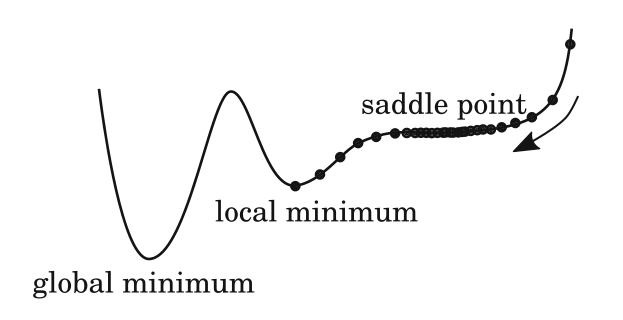
\includegraphics[width=10cm]{latex/figures/local_minimum_saddle_point.png}
    \caption{One-dimensional representation of the loss landscape for a parameterized model, showcasing the phenomenon of getting stuck in local minima, and slow convergence induced by plateaus. The figure is retrieved from \citet{géron2017hands-on.}}
    \label{fig:localMinima}
\end{figure}

\begin{figure}[htp]
    \centering
    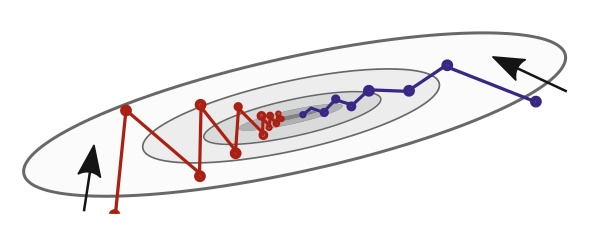
\includegraphics[width=8cm]{latex/figures/thin_vally.png}
    \caption{Two-dimensional representation of the loss landscape for a parameterized model, illustrating a thin valley. The optimization steps in red showcase optimization without momentum. Optimization steps in blue implement momentum, showing dampened oscillation and better convergence. The figure is retrieved from \citet{SupervisedwquantumComputers}.}
    \label{fig:thinValley}
\end{figure}

%================================================================
\subsection{Adam Optimizer}\label{sec:AdamOptimizer}
%================================================================
Introduced by \citet{kingma2017adam}, the Adam algorithm implements a moving average of the gradient, called \emph{momentum}, together with a rescaling. Replacing \autoref{eq:Gradient} and \autoref{eq:ParameterUpdate}, Adam implements the following algorithm:

\begin{algorithm}[H]\label{alg:Adam}
\SetAlgoLined

$m_0 \gets 0$;\\
$v_0 \gets 0$;\\
$t \gets 0$;\\
\While{$\theta_t$ not converged}{
t \gets t+1\\
$g_t \gets \nabla_{\theta} L(\theta_{t-1})$
(Get gradients w.r.t. loss at timestep t)\\
$m_t \gets \beta_1 m_{t-1} + (1-\beta_1) g_{t}$
(Update biased first moment estimate)\\
$v_t \gets \beta_2 v_{t-1} + (1-\beta_2) g_{t}^2$
(Update biased second raw moment estimate)\\
$\hat{m}_t \gets m_t/(1 - \beta_1^{t})$
(Compute bias-corrected first moment estimate)\\
$\hat{v}_t \gets v_t/(1 - \beta_2^{t})$
(Compute bias-corrected second raw moment estimate)\\
$\theta_t \gets \theta_{t-1} - \alpha \hat{m}_t/(\sqrt{\hat{v}_t} + \epsilon)$
(Update parameters)
}\Return{$\theta_t$}
\caption{\emph{Adam}, \cite{kingma2017adam}. The authors suggest default hyperparameters $\alpha = 0.001$, $\beta_1 = 0.9$, $\beta_2 = 0.999$ and $\epsilon = 10^{-8}$. The algorithm is applied parameter-wise.}
\end{algorithm}

\autoref{alg:Adam} updates moving averages of the gradient $m_t$ and its square $v_t$, picking up information about the gradient from earlier update events. In particular, if the gradient tend to flip sign for certain directions, the averaging over previous iterations tends to dampen these oscillations. Likewise, directions of persistent sign tends to accumulate magnitude, making the optimisation gain "momentum" in these directions. This is a good property for overcoming thin valleys and plateaus. Also, the effect of momentum may also help avoid getting stuck in local minima by gracing over them. Further, the moving average of the gradient and its square is rendered unbiased as $\hat{m}_t = m_t/(1-\beta_1)$ and $\hat{v}_t = v_t/(1-\beta_2)$. Since the averages are initialized as zero, they are biased downward. Finally, the parameters are shifted by the quantity $\alpha \frac{\hat{m}_t}{\sqrt{\hat{v}_t} + \epsilon}$. Here, the rescaling term $\sqrt{\hat{v}_t}$ serves to decrease the step size in directions where the gradient has a large magnitude and increase it where it is small. This effectively implements a variable learning rate for each direction, depending on whether big or small steps are needed. 

Adam is a hugely successful algorithm for optimizing machine learning models. In popular machine learning frames such as scikit-learn \cite{scikit-learn} and pyTorch \cite{NEURIPS2019_9015}, it is a default optimizer. Lately, Adam has also been used for optimizing quantum machine learning models \cite{abbas2020power} \cite{skolik2020layerwise}. Pointed out by its authors, Adam requires very little tuning of hyper-parameters to be efficient, making attractive and easy to use. Adam is also suited for noisy gradients, which will be relevant for the work in this thesis. 



%================================================================
\section{Dense Neural Network}\label{sec:DenseNeuralNetwork}
%================================================================
Originally inspired by the network structure of the brain(kilde?), artificial neural networks are powerful parameterized machine learning models that have proved to extremely useful for a vast number of applications. Over the years, a comprehensive collection of different network architectures have been developed to target specific problems, such as \emph{Recurrent Neural Networks} for predicting time series data and \emph{Convolutional Neural Networks} for image classification. In this thesis, we focus on \emph{Dense Neural Networks}, which is a type of simple \emph{feedforward network}, meaning the information is processed in a forward fashion without any loops that direct information backwards.

%================================================================
\subsection{Feedforward}\label{sec:FeedforwardDNN}
%================================================================
Dense Neural Networks work by sequentially transforming input data by passing them through one or more \emph{layers}, which each applies a parameterized and often non-linear transformation. The result of the first layer of the neural network can be formulated as

\begin{equation}\label{eq:FeedforwardSingle}
    \boldsymbol{a}^1 = f^1(\boldsymbol{z}^1) = f^1(W^1 \boldsymbol{x} + \boldsymbol{b}^1),
\end{equation}
Here, $\boldsymbol{x} \in \mathbb{R}^p$ is a single sample of $p$ features. $W^1 \in \mathbb{R}^{m \times p}$ and $\boldsymbol{b}^1 \in \mathbb{R}^{m}$ are a matrix and a vector of parameters called the \emph{weights} and \emph{biases}, respectively. The operations $W^1 \boldsymbol{x} + \boldsymbol{b}^1$ applies an affine transformation of the features resulting in $m$ new derived features, each identified as a \emph{node} in the specific layer. Further, $f^1(\cdot)$ is a layer-specific function, often monotonous and non-linear, applied element-wise on the derived features. This finally results in the output of the layer, $\boldsymbol{a}^1$, called the \emph{activation}.

We will now generalize \autoref{eq:FeedforwardSingle} to an arbitrary layer. For a neural network with $L$ layers, the feedforward procedure for layer $l$  can be formulated as 

\begin{equation}\label{eq:FeedforwardDNN}
    \boldsymbol{a}^l = f^l(\boldsymbol{z}^l) = f^1(W^l \boldsymbol{a^{l-1}} + \boldsymbol{b}^l),
\end{equation}
where $\boldsymbol{a}^{l-1}$ is the activation of the previous layer with the exception $\boldsymbol{a}^{0} = \boldsymbol{x}$. The output of the network is then the activation of the last layer, namely 
\begin{equation}\label{eq:DNN}
    \hat{y} = f_{DNN}(x;\boldsymbol{\theta}) = \boldsymbol{a}^{L},
\end{equation}
where $\boldsymbol{\theta} = [W^1, \boldsymbol{b}^1, \cdots, W^L,  \boldsymbol{b}^L]$. This defines the whole forward procedure of a neural network, and also highlights the role of the functions $f^l(\cdot)$, often called the \emph{non-linearities}. If set to identity, $f^l(x) = x$, the recursive application of \autoref{eq:FeedforwardDNN} would simply apply repeated affine transformations, which is an affine transformation in itself. In other words, increasing the number of layers would not increase the expressiveness of the network, as all the layers would collapse into a single layer. Therefore, introducing non-linear transformations is necessary to increase the flexibility of the neural network(kilde?). 

%================================================================
\subsection{Backpropagation}\label{sec:BackpropogationDNN}
%================================================================

%Neural networks are typically trained using gradient-based methods, such as Batch Gradient Descent and Adam, both previously discussed. Adam is particularly efficient, as the optimization of neural network architectures tend to be plagued by many local minima and plateaus(kilde).  

Assume that $f(\boldsymbol{x}^{(i)}; \boldsymbol{\theta})$ is a dense neural network as described by \autoref{eq:FeedforwardDNN} and \autoref{eq:DNN}. In order to use gradient-based methods, one needs to calculate the derivative of the loss-function \autoref{eq:LossDerivateWRTparameter} for an arbitrary parameter $\boldsymbol{\theta}_k$, which could be any of the weights $W^l$ or biases $\boldsymbol{b}^l$ in the various layers. This is not trivial given the sequential structure of the neural network. Often attributed to \citet{Rumelhart}, the \emph{backpropagation algorithm} calculates the gradient in a sequential manner, starting with the last layers first. Calculating on a single sample, the algorithm starts by calculating the \emph{error} of the last layer


\begin{equation}\label{eq:lastLayerError}
    \delta^L_k = \frac{\partial L(\hat{y}, y)}{\partial \boldsymbol{a}^L_k},
\end{equation}
where $k$ indicates the node.

This error can be defined for any layer recursively by repeated application of the chain-rule:
\begin{equation}\label{eq:error}
    \delta^l_j = \frac{\partial L(\hat{y}, y)}{\partial \boldsymbol{a}^l_j} 
    = \sum_k \frac{\partial L(\hat{y}, y)}{\partial \boldsymbol{a}^{l+1}_k} \frac{\partial \boldsymbol{a}^{l+1}_k}{\partial \boldsymbol{a}^{l}_j}
    = \sum_k \delta^{l+1}_k \frac{\partial \boldsymbol{a}^{l+1}_k}{\partial \boldsymbol{a}^{l}_j}.
\end{equation}
This relation is the origin of the name \emph{backpropogation}, as the error terms $\delta^l$ "propagate" backwards through the neural network as they are calculated.

Using that 
$\frac{\partial \boldsymbol{a}^{l}_k}{\partial W^l_{ij}} = f^{l\prime}(\boldsymbol{z}^{l}_k)\boldsymbol{a}^{l-1}_j I_{ik}$ 
and 
$\frac{\partial \boldsymbol{a}^{l}_k}{\partial \boldsymbol{b}^l_{i}} = f^{l\prime}(\boldsymbol{z}^{l}_k) I_{ik}$, the derivative with respect to the weights and biases can then be calculated as 

\begin{equation}\label{eq:derivweights}
    \frac{\partial L(\hat{y}, y)}{\partial W^l_{ij}} = 
    \sum_k \frac{\partial L(\hat{y}, y)}{\partial \boldsymbol{a}^{l}_k} \frac{\partial \boldsymbol{a}^{l}_k}{\partial W^l_{ij}} = 
    \sum_k \delta^{l}_k f^{l\prime}(\boldsymbol{z}^{l}_k)\boldsymbol{a}^{l-1}_j I_{ik}=
    \delta^{l}_i f^{l\prime}(\boldsymbol{z}^l_i) \boldsymbol{a}^{l-1}_j,
\end{equation}
and
\begin{equation}\label{eq:derivbiases}
    \frac{\partial L(\hat{y}, y)}{\partial \boldsymbol{b}^l_{i}} = 
    \sum_k \frac{\partial L(\hat{y}, y)}{\partial \boldsymbol{a}^{l}_k} \frac{\partial \boldsymbol{a}^{l}_k}{\partial \boldsymbol{b}^l_{i}} = 
    \sum_k \delta^{l}_k f^{l\prime}(\boldsymbol{z}^{l}_k)\boldsymbol{a}^{l-1}_j I_{ik}=
    \delta^{l}_i f^{l\prime}(\boldsymbol{z}^l_i).
\end{equation}

The final gradient, over all samples, is then the average of all the single-sample gradients

\begin{equation}\label{eq:averageGradient}
    \nabla_{\boldsymbol{\theta}} L(\boldsymbol{\theta}) = \frac{1}{N}\sum_{i=1}^N \nabla_{\boldsymbol{\theta}} L(\hat{y}^{(i)}, y^{(i)}),
\end{equation}
which can be used to optimize the neural network with a gradient-based method as discussed earlier.


%================================================================
\section{Generalizability}\label{sec:Generalizability}
%================================================================
If we obtain a low loss on the training data after fitting a model, can we assume that the resulting model is good and useful? It depends on what we want to use the model for, but if we want to use the model for predicting on new data (data that was not seen during training), we often don't want train the model too much. As explained earlier, the main goal of a model is to approximate the underlying mechanism $f(\boldsymbol{x})$ producing the data. If the model fits the data too hard, it might also pick up details of the noise $\epsilon$ in the training data, which is called \emph{overfitting}. The problem with this is that if we gather a new data set, a \emph{test set} $y' = f(\boldsymbol{x}) + \epsilon'$, the noise $\epsilon'$ will be different from the noise in the training data because of its random nature. Since the overfitted model is very affected by the noise in the training data, it will likely perform badly on new data where the noise is different, even though its performance on the training data is good. Typically, the more complex and flexible a model is, the more likely it is to overfit the training data. This is because it has a greater capacity to fit the noise present in the training data. By restricting the complexity of the model, one often ends up with a model that resembles $f(\boldsymbol{x})$ more closely. In turn, this results in a model
that \emph{generalizes} better, which means that it makes accurate predictions on values of $\boldsymbol{x}$ not seen in the training set. On the other hand, if the model is made not complex enough, it might not be sufficiently flexible to recreate $f(\boldsymbol{x})$, causing \emph{underfitting}.

To uncover overfitting, it is standard procedure to prepare independent training and test data sets $\mathcal{T}_{Train}$ and $\mathcal{T}_{Test}$, and train the model on the former set and test its performance on the latter. 


%================================================================
\section{Pre-processing Features}\label{sec:Pre-processing Features Theory}
%================================================================
In this section, we will discuss 

%================================================================
\subsection{Standardization}\label{sec:Standardization}
%================================================================
For data sets gathered for real world applications, it is often the case that the different features 

%================================================================
\subsection{Principal Component Analysis}\label{sec:Principal Component Analysis}
%================================================================

%================================================================
\chapter{Quantum Computing}\label{chap:QuantumComputing}
%================================================================
This chapter introduces the fundamentals of quantum computing. The content of this chapter is mainly based on material in \citet{NielsenQuantum}.


%================================================================
\section{States in Quantum Mechanics}\label{sec:IntroQM}
%===============================================================
In quantum mechanics, isolated physical systems are described completely by its \emph{state vector}, which lives in a complex vector space. In this thesis, we will focus on finite vector spaces $\mathbb{C}^n$, where states are n-tuples of complex numbers $(z_1, \cdots, z_n)$ called \emph{amplitudes}. Adopting Dirac notation, a state is denoted as 
\begin{equation}
    \ket{\psi} \sim \begin{bmatrix}
           z_{1} \\
           \vdots \\
           z_{n}
         \end{bmatrix},
\end{equation}
where $\psi$ is the label of the state, and $\ket{\cdot}$ indicates that it is a vector. More specifically, in quantum mechanics, the states live in \emph{Hilbert space}, which is a vector space that has a well-defined inner product. The inner product of two states $\ket{\psi}, \ket{\psi'} \in \mathbb{C}^n$ is denoted 

\begin{equation}
    \braket{\psi'}{\psi} \equiv [z_1'^*, \cdots, z_n'^*] 
    \begin{bmatrix}
        z_{1} \\
        \vdots \\
        z_{n}
    \end{bmatrix}
    = \sum_{i=1}^{n} z_i'^* z_i, 
\end{equation}
where $z^*$ indicates the complex conjugate. That is, if $z = a + ib$, the complex conjugate results in $z^* = a - ib$. As a constraint on the amplitudes, state vectors that describe physical systems have unit norm, meaning 

\begin{equation}
    \braket{\psi}{\psi} \equiv [z_1^*, \cdots, z_n^*] 
    \begin{bmatrix}
        z_{1} \\
        \vdots \\
        z_{n}
    \end{bmatrix}
    = \sum_{i=1}^{n} |z_i|^2 = 1.
\end{equation}

%================================================================
\subsection{The Qubit}\label{sec:TheQubit}
%===============================================================
As is common in quantum computing, we will focus on perhaps the simplest possible quantum system, the \emph{qubit}, which is a two-level system defined on $\mathbb{C}^2$.  There are multiple ways of implementing qubits in hardware, some of which will be discussed later, although  the specific physical realization is not necessary to account for when discussing quantum computing. In abstract terms, the state of a qubit can be formulated as

\begin{equation}
\ket{\psi} = \alpha \ket{0} + \beta \ket{1},
\end{equation}
where $\alpha$ and $\beta$ are complex numbers, and $\ket{0}$ and $\ket{1}$ are orthonormal states known as the \emph{computational basis states} and are defined by the implementation of the hardware. This linear combination of states is an important principle of quantum mechanics and is called \emph{superposition}; the system is in neither state $\ket{0}$ nor $\ket{1}$, but both at the same time(unless either $\alpha$ or $\beta$ is zero). In general, if states $\ket{\psi}$ and $\ket{\phi}$ are allowed, then so is the linear combination $\alpha \ket{\psi} + \beta \ket{\phi}$, where $|\alpha|^2 + |\beta|^2 = 1$.

Being the "atom" of quantum computing, the qubit is reminiscent of the classical bit, which is always definitely "0" or "1". However, as we have seen, the qubit also may assume any normalized linear combination of the two states.
%================================================================
\subsection{Multiple Qubits}\label{sec:Multiple Qubits}
%===============================================================
As a central property of quantum mechanics, it is possible to create composite systems by combining several smaller quantum systems. This can be used to construct systems of multiple qubits, whose collective state can be expressed, if the qubits are independent, as

\begin{equation}\label{eq:tensorProductState}
\ket{\psi_1 \psi_2 \cdots \psi_n} \equiv \ket{\psi_1} \otimes \ket{\psi_2} \otimes \cdots \ket{\psi_n}.
\end{equation}
Here, the tensor product "$\otimes$" was used to indicate that each state $\ket{\psi_i}$ lives in its own $\mathbb{C}^2$ space. Using the principle of superposition, one may make a linear combination of several multi-qubit states, where each $\ket{\psi_i}$ is either $\ket{0}$ or $\ket{1}$. In general, this can be written as

\begin{equation}\label{eq:MultiQubitState}
\ket{\psi} = \sum_{\boldsymbol{v}}c_{\boldsymbol{v}}\ket{\boldsymbol{v}_1} \otimes \ket{\boldsymbol{v}_2} \otimes \cdots \ket{\boldsymbol{v}_n},
\end{equation}
where $\boldsymbol{v} \in \{0,1\}^n$ sums over all possible binary strings of length $n$. As there are $2^n$ unique strings, we arrive at the remarkable result that one also needs $2^n$ amplitudes $c_{\boldsymbol{v}}$ to describe the state of $n$ qubits in general. In other words, the information stored in the quantum state of $n$ qubits is exponential in $n$, as opposed to the linear information of an equivalent classical system of classical bits. In a sense, the quantum information is "larger" than the classical information. This is a fascinating property of the  capabilities of quantum computing, which we will return to when discussing the usefulness of quantum computing in relation to machine learning.

%================================================================
\subsection{Measuring Qubits}\label{sec:MeasuringState}
%===============================================================
It appears the information encoded in quantum systems is much greater than the information in a corresponding classical system, at least in the case of qubits versus bits. How can one interact with this information? Unlike classical bits, whose state can always be measured exactly, the state of one or multiple qubits cannot be measured and determined. Returning to the single qubit example, one can choose to perform a measurement in the computational basis on a qubit in the state $\ket{\psi} = \alpha \ket{0} + \beta \ket{1}$. The measurement will result in  \emph{either} $\ket{0}$ \emph{or} $\ket{1}$, with probabilities $|\alpha|^2$ and $|\beta|^2$, respectively. For multiple qubits in a general state \cref{eq:MultiQubitState}, a measurement on all qubits will grant a state in the computational basis, i.e. $\ket{\boldsymbol{v}_1} \otimes \ket{\boldsymbol{v}_2} \otimes \cdots \ket{\boldsymbol{v}_n}$ for some binary string $\boldsymbol{v} \in \{0,1\}^n$, with probability $|c_{\boldsymbol{v}}|^2$. This motivates why states in quantum mechanics need to have unity norm, i.e
\begin{equation}\label{eq:MultiQubitState}
\sum_{\boldsymbol{v}}|c_{\boldsymbol{v}}|^2 = 1,
\end{equation} 
as the probabilities of any outcome must sum to $1$.

%================================================================
\section{Quantum Circuits}\label{sec:QuantumCircuits}
%===============================================================
We have discussed how quantum states can encode information, and how to interact with information through measuring the state. How then can quantum mechanics be used for computation? In order to perform computations, it is necessary to introduce some dynamical transformation of the quantum state. In quantum mechanics, transformations can be formulated as 

\begin{equation}\label{eq:UnitaryEvolution}
 \ket{\phi} = U\ket{\psi},
\end{equation}
where $U$ is a \emph{unitary} operator that acts on the vector space where $\ket{\psi}$ and $\ket{\phi}$ live. "Unitary" means that the operator $U$ is linear with the property that $U^{\dagger} = U^{-1}$, that is, the Hermitian conjugate is equal to its inverse. This is a necessary property of linear operators in quantum mechanics as to ensure that the state stays normalized to 1:

\begin{equation}\label{eq:UnitaryEvolution}
 \braket{\phi}{\phi} = \bra{\psi}\underset{I}{\underbrace{U^{\dagger}U}}\ket{\psi} = \bra{\psi}\ket{\psi} =1.
\end{equation}
Assuming $\ket{\psi}$ is initially normalized, so is $\ket{\phi}$ after a unitary transformation.

By construction, quantum computers allow for the application of carefully selected sequences of operators that transform the state in a desired way, often called a \emph{quantum circuit}. Typical operators used in quantum computing, often called quantum gates, act on one or multiple qubits, and are analogous to logical operations in the classical context. 

\cref{fig:exampleCircuit} illustrates an example of a quantum circuit. Going from left to right indicates the chronological order of application of the different quantum gates. Note that the exact passing of time is not shown in this schematic, and is highly dependent on the implementation of physical hardware. The horizontal lines, called wires, each symbolize a qubit. The qubits are initialized in the zero state, as shown by the notation on the left-hand side. Then, various gates are applied to the qubits, acting on one, two or three qubits. Lastly, illustrated by the gauge symbol, each qubit is measured in the computational basis, yielding either $0$ or $1$. This information is then stored in the classical register $c$, indicated by the double line. 

\begin{figure}[htp]
    \centering
    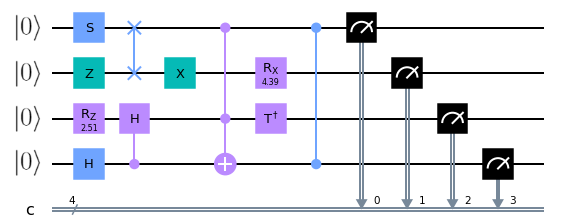
\includegraphics[width=10cm]{latex/figures/example_circuit.png}
    \caption{Example circuit consisting of 4 qubits initialized to $\ket{0}$. A random selection of quantum gates acting on one, two and three qubits are then applied. Finally, all qubits are measured in the computational basis and stored in a classical register.}
    \label{fig:exampleCircuit}
\end{figure}

%================================================================
\subsection{Single Qubit Operations}\label{sec:ControlledOperations}
%===============================================================

Returning again to the single qubit, the state of a qubit can be represented as a vector
\begin{equation}\label{eq:vectorRepresentation}
\ket{\psi} = \alpha \ket{0} + \beta \ket{1} \equiv \alpha 
    \begin{bmatrix}
        1 \\
        0
    \end{bmatrix} + 
    \beta \begin{bmatrix}
        0 \\
        1
    \end{bmatrix}
    =
    \begin{bmatrix}
        \alpha \\
        \beta
    \end{bmatrix}.
\end{equation}
Likewise, linear operators acting on a single qubit can in general be represented by a $2\times 2$ matrix 
\begin{equation}\label{eq:matrixRepresentation}
    \begin{bmatrix}
        c_{11} & c_{12} \\
        c_{21} & c_{22}
    \end{bmatrix},
\end{equation}
which is unitary. A particularly interesting single qubit quantum gate is the Hadamard gate, which is formulated as 

\begin{equation}\label{eq:matrixRepresentation}
    H = \frac{1}{\sqrt{2}}\begin{bmatrix}
        1 & 1 \\
        1 & -1
    \end{bmatrix} = 
    \Qcircuit @C=1em @R=.7em {& \gate{H} & \qw}\\.
\end{equation}
Acting on the computational basis, the Hadamard gate can be seen to produce superpositions
\begin{align*}
    H\ket{0} = \frac{1}{\sqrt{2}}\ket{0} +\frac{1}{\sqrt{2}}\ket{1}\\
    H\ket{1} = \frac{1}{\sqrt{2}}\ket{0} -\frac{1}{\sqrt{2}}\ket{1},
\end{align*}
which gives a $50\%$ chance to yield either $0$ or $1$ upon measuring. In a sense, this is the quantum mechanical equivalent to a coin toss. Contrary to a coin toss, if applied a second time, we return to the original state, "unscrambling" the coin, or qubit:

\begin{equation}\label{eq:unscramble}
    HH\ket{0} = \frac{1}{\sqrt{2}}H\ket{0} +\frac{1}{\sqrt{2}}H\ket{1} = \frac{1}{2}(\ket{0} + \ket{0}) + \frac{1}{2}(\ket{1} - \ket{1}) = \ket{0}.
\end{equation}
As pointed out in \citet{SupervisedwquantumComputers}, this phenomenon has no classical equivalent. If one has a classical procedure of scrambling a coin, e.g. shaking it in your hands, a second shaking will not leave it unscrambled, but scrambled still. Quantum computation is able to reverse this because quantum mechanics is fundamentally not a theory of probabilities; Probabilities can be derived from the theory, but the underlying description revolves around amplitudes, as explained earlier. Whereas probabilities must be positive or zero, amplitudes can be positive or negative(and complex in general), which allows destructive interference. This can be seen in \cref{eq:unscramble}, where the last term $\frac{1}{2}(\ket{1} - \ket{1})$ is cancelled out. In addition to the exponentially large size of Hilbert space, this is also an interesting property of quantum computing when discussing its capabilities over classical computing.

Further, a much-used set of single qubit gates are the Pauli operators:

\begin{equation}
\begin{aligned}
    X = \sigma_x = 
    \begin{bmatrix}
        0 & 1 \\
        1 & 0
    \end{bmatrix} = 
    \Qcircuit @C=1em @R=.7em {& \gate{X} & \qw}\\
    Y = \sigma_y = 
    \begin{bmatrix}
        0 & -i \\
        i & 0
    \end{bmatrix} = 
    \Qcircuit @C=1em @R=.7em {& \gate{Y} & \qw}\\
    Z = \sigma_z = 
    \begin{bmatrix}
        1 & 0 \\
        0 & -1
    \end{bmatrix} = 
    \Qcircuit @C=1em @R=.7em {& \gate{Z} & \qw}
\end{aligned}    
\end{equation}

To visualize what these operators do, it is useful to introduce a geometrical representation called the \emph{Bloch sphere}, illustrated in \cref{fig:blochsphere}. Rewriting the state of a qubit to 

\begin{equation}\label{eq:blochsphere}
    \ket{\psi} = \alpha \ket{0} + \beta \ket{1} = e^{i\gamma}(\cos{\frac{\theta}{2}}\ket{0} + e^{i\phi}\sin{\frac{\theta}{2}}\ket{1}) \sim 
    \cos{\frac{\theta}{2}}\ket{0} + e^{i\phi}\sin{\frac{\theta}{2}}\ket{1},
\end{equation}
the new parameters $\theta$ and $\phi$ can be identified as the azimuthal and polar angles, respectively. Here, the factor $e^{i\gamma}$ is known as a global phase, which is not physically important to include. Using this, any single qubit state can then be identified as a point on the Bloch sphere.

\begin{figure}[htp]
    \centering
    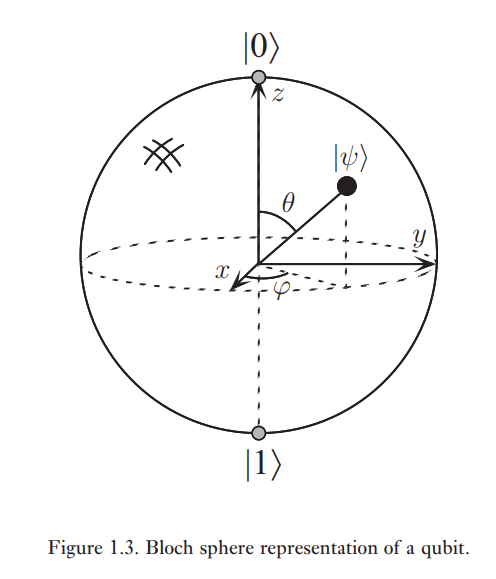
\includegraphics[width=10cm]{latex/figures/Blochsphere.PNG}
    \caption{Geometrical representation of the state of a qubit, called the Bloch sphere. The figure is retrieved from \citet{NielsenQuantum}.}
    \label{fig:blochsphere}
\end{figure}

The Pauli-gates represent a $180^{\circ}$ rotation of the state around the corresponding axis. Particularly, the $X$ gate, often called the \emph{flip gate}, acts on the basis states as

\begin{equation}
\begin{aligned}
    X\ket{0} &= \ket{1} \\
    X\ket{1} &= \ket{0} \\
    X(\alpha \ket{0} + \beta\ket{1}) &= \beta \ket{0} + \alpha\ket{1}.
\end{aligned}    
\end{equation}
Much like how the classical NOT-gate flips the bit, the X gate flips the qubit.

Another essential set of gates used for quantum machine learning, which can be derived from the aforementioned Pauli gates, are the \emph{Pauli rotations}. They are formulated as exponentiated Pauli gates in the following way:

\begin{equation}\label{eq:PauliRotations}
\begin{aligned}
    R_x(\theta) = e^{-i\theta\sigma_x/2} = \cos{\frac{\theta}{2}}I - i\sin{\frac{\theta}{2}}\sigma_x
    =
    \begin{bmatrix}
        \cos{\frac{\theta}{2}} & -i\sin{\frac{\theta}{2}} \\
        -i\sin{\frac{\theta}{2}} & \cos{\frac{\theta}{2}}
    \end{bmatrix}\\
    R_y(\theta) = e^{-i\theta\sigma_y/2} = \cos{\frac{\theta}{2}}I - i\sin{\frac{\theta}{2}}\sigma_y
    =
    \begin{bmatrix}
        \cos{\frac{\theta}{2}} & -\sin{\frac{\theta}{2}} \\
        \sin{\frac{\theta}{2}} & \cos{\frac{\theta}{2}}
    \end{bmatrix}\\
    R_z(\theta) = e^{-i\theta\sigma_z/2} = \cos{\frac{\theta}{2}}I - i\sin{\frac{\theta}{2}}\sigma_z
    =
    \begin{bmatrix}
        e^{-i\theta/2} & 0 \\
        0 & e^{i\theta/2}
    \end{bmatrix}\\.
\end{aligned}    
\end{equation}

The action of a gate $R_j(\theta)$ on a state, for $j \in \{x,y,z\}$, is to rotate the state around the $j$-axis on the Bloch sphere, for an amount of $\theta$ radians. As $\theta$ can be any real number, these gates can be viewed as being quantum gates parameterized by $\theta$, which will be an essential component when we will construct \emph{parameterized quantum circuits} later.

%================================================================
\subsection{Multi-Qubit Operators}\label{sec:ControlledOperations}
%===============================================================
With only single qubit gates, the number of states we can access is greatly reduced as all the qubits stay independent, i.e. the state can be written as \cref{eq:tensorProductState}. By introducing gates that operate on several qubits, one can for example transform the state of one qubit conditioned on the state of an other qubit. This makes the two qubits correlated, known as \emph{entanglement} in quantum mechanics.

\subsubsection*{CNOT}
One such conditional gate is the controlled NOT gate (CNOT gate). It is formulated as

\begin{equation}
    CNOT = 
    \ket{0}\bra{0}\otimes I + \ket{1}\bra{1}\otimes X =
    \begin{bmatrix}
        1 & 0 & 0 & 0 \\
        0 & 1 & 0 & 0 \\
        0 & 0 & 0 & 1 \\
        0 & 0 & 1 & 0
    \end{bmatrix}
    = 
    \begin{array}{c}
    \Qcircuit @C=1em @R=.7em {
    & \ctrl{1} & \qw \\
    & \targ  & \qw
    }
    \end{array},
\end{equation}
where we have also included its formulation in Dirac notation. Looking at the circuit representation, the black dot indicates that the gate is conditioned on the top qubit(control qubit). If it is in state $\ket{1}$, an $X$ gate is applied to the bottom qubit(target qubit). Otherwise, it is left unchanged. By convention, the X gate here is denoted by $\bigoplus$. This operation has an interesting effect if the control qubit is in a superposition. Assume we begin in the state
\begin{equation}
    \ket{\psi} = H\ket{0}\otimes\ket{0} = \frac{1}{\sqrt{2}}(\ket{0} + \ket{1})\otimes\ket{0},
\end{equation} the application of the CNOT gate will yield the following:

\begin{equation}
    CNOT\ket{\psi} =
    \frac{1}{\sqrt{2}}(\ket{0}\otimes I\ket{0} + \ket{1}\otimes X\ket{0}) =
    \frac{1}{\sqrt{2}}(\ket{0}\otimes \ket{0} + \ket{1}\otimes \ket{1}).
\end{equation}
This is a well-known state called a \emph{Bell state}. It has the interesting property that the qubits are correlated: When the first qubit is measured to be in either state $0$ or $1$, the second qubit will be found in the same state, and vice versa. This is known as an entangled state, which cannot be expressed as a product of independent single qubit states, such as \cref{eq:tensorProductState}. By introducing controlled gates, we have increased the space of accessible states.

\subsubsection*{Multi-Controlled Gate}
The CNOT gate is just one example of a controlled quantum gate. In general, we can have a controlled gate on the form 

\begin{equation}
    \ket{0}\bra{0}\otimes I + \ket{1}\bra{1}\otimes U
    = 
    \begin{array}{c}
    \Qcircuit @C=1em @R=.7em {
    & \ctrl{1} & \qw \\
    & \gate{U}  & \qw
    }
    \end{array},
\end{equation}
where U is any single qubit gate. Moreover, there also exists \emph{multi-controlled gates} on the form

\begin{equation}
    \begin{array}{c}
    \Qcircuit @C=1em @R=.7em {
    & \ctrl{1} & \qw \\
    & \ctrl{1} & \qw \\
    & \ctrl{1} & \qw \\
    & \gate{U}  & \qw
    }
    \end{array}.
\end{equation}
This gate applies $U$ to the target qubit if, and only if, all three control qubits(in general $n$ control qubits) are in state $\ket{1}$. The application of the gate may be dependent on the control qubits being in $\ket{0}$ rather that $\ket{1}$. This can be done by applying an $X$ gate before and after the controlled operation to the qubit one wishes to invert, such as  

\begin{equation}
    \begin{array}{c}
    \Qcircuit @C=1em @R=.7em {
            & \ctrl{1} & \qw \\
    \gate{X}& \ctrl{1} & \gate{X} \\
            & \ctrl{1} & \qw \\
            & \gate{U} & \qw
    }
    \end{array}=
    \begin{array}{c}
    \Qcircuit @C=1em @R=.7em {
    & \ctrl{1} & \qw \\
    & \ctrlo{1} &  \qw \\
    & \ctrl{1} & \qw \\
    & \gate{U}  & \qw
    }
    \end{array}.
\end{equation}
Here, the conditioning on state $\ket{0}$ is indicated by a white dot.

\subsubsection*{SWAP gate}
A well-known two-qubit gate is the SWAP gate. As the name indicates, the SWAP gate swaps the information of qubits. It is defined as 

\begin{equation}
    SWAP = 
    \begin{bmatrix}
        1 & 0 & 0 & 0 \\
        0 & 0 & 1 & 0 \\
        0 & 1 & 0 & 0 \\
        0 & 0 & 0 & 1
    \end{bmatrix}
    = 
    \begin{array}{c}
    \Qcircuit @C=1em @R=1.3em {
    & \qswap & \qw \\
    & \qswap \qwx & \qw
    }
    \end{array},
\end{equation}
For a two-qubit system, where the first qubit is in the state $\ket{\psi}$ and the second is in $\ket{\phi}$, the swap gate has the following function:

\begin{equation}
    \begin{array}{c}
    \Qcircuit @C=1em @R=1.3em {
    \lstick{\ket{\psi}}& \qswap & \rstick{\ket{\phi}} \qw \\
    \lstick{\ket{\phi}}& \qswap \qwx  & \rstick{\ket{\psi}} \qw
    }
    \end{array}
\end{equation}




%================================================================
\subsection{Observables}\label{sec:Observables}
%===============================================================
In \cref{sec:MeasuringState}, we introduced the process of measurement. We will now generalize this by introducing \emph{quantum observables}. In quantum mechanics, an observable is an operator that acts on the state space of the system being measured. It can be expressed as
\begin{equation}\label{eq:observable}
    \hat{O} = \sum_m m P_m,
\end{equation}
where $m$ are real numbers called \emph{eigenvalues} and $P_m$ are projection operators(satisfying $P_m^2 = P_m$) with the condition $\sum_m P_m = I$. Under these conditions, the operator $\hat{O}$ is said to be \emph{Hermitian}, which is a property required of all quantum observables. Upon measuring the observable \cref{eq:observable} on a state $\ket{\psi}$, the measured value will be $m$ with probability 

\begin{equation}
    p(m) = \bra{\psi}P_m\ket{\psi},
\end{equation}

and original state will be projected onto $P_m$ yielding 

\begin{equation}
    \ket{\psi} \rightarrow \frac{P_m\ket{\psi}}{\sqrt{\bra{\psi}P_m\ket{\psi}}},
\end{equation}
where the scaling factor ensures that the new state is still normalized. Using this formalism, one can identify the Pauli gate $\sigma_z$ as a suitable observable for measuring the computational basis:

\begin{equation}
    \sigma_z = \ket{0}\bra{0} - \ket{1}\bra{1}.
\end{equation}

For the general single qubit state $\ket{\psi} = \alpha \ket{0} + \beta \ket{1}$, we see that probabilities of measuring $m=1$ and $m=-1$ are respectively

\begin{equation}
\begin{aligned}
    p(0) = \bra{\psi} \ket{0}\bra{0} \ket{\psi} = (\alpha^* \bra{0} + \beta^* \bra{1}) \ket{0}\bra{0} (\alpha \ket{0} + \beta \ket{1}) = |\alpha|^2,\\
    p(1) = \bra{\psi} \ket{1}\bra{1} \ket{\psi} = (\alpha^* \bra{0} + \beta^* \bra{1}) \ket{1}\bra{1} (\alpha \ket{0} + \beta \ket{1}) = |\beta|^2,
\end{aligned}
\end{equation}

and the states after the corresponding measurement is 


\begin{equation}\label{eq:CompBasisMeasurement}
\begin{aligned}
    \frac{\ket{0}\bra{0}(\alpha \ket{0} + \beta \ket{1})}{\sqrt{|\alpha|^2}} = 
    \frac{\alpha}{|\alpha|} \ket{0} \sim \ket{0} \\
    \frac{\ket{1}\bra{1}(\alpha \ket{0} + \beta \ket{1})}{\sqrt{|\beta|^2}} = 
    \frac{\beta}{|\beta|} \ket{1} \sim \ket{1},
\end{aligned}
\end{equation}
where it was used that $\frac{\alpha}{|\alpha|}$ and $\frac{\beta}{|\beta|}$ are just global phases, and hence not important. Thus we see that the measurement leaves the state in the computational basis corresponding with the measured value, with the correct probability as described in \cref{sec:MeasuringState}.

%================================================================
\subsection{Expectation Values}\label{sec:ExpectationValues}
%===============================================================

What is the average value of an observable for a given state $\ket{\psi}$? Using statistical formalism, we can formulate this as the \emph{expectation values} of the observable

\begin{equation}\label{eq:ExpectedValue}
    \mathbb{E}(m) = \sum_m m p(m) = \sum_m m \bra{\psi}P_m\ket{\psi} = \bra{\psi}\sum_m m P_m\ket{\psi} = \bra{\psi}\hat{O}\ket{\psi},
\end{equation}

where $\bra{\psi}\hat{O}\ket{\psi}$ is a recurring expression in quantum mechanics, often denoted simply as $\langle \hat{O} \rangle$. The expectation value is crucial for quantum computing as it serves as a method for extracting a deterministic value from a quantum state. Whereas the total quantum information of a state is inaccessible to us, estimating the expectation value for some desired observable is possible for retrieving an output of a quantum algorithm. Desirably, this output serves as a solution to the problem one wishes to solve. Looking at the expected value \cref{eq:ExpectedValue}, it is easy to see why global phases of the state are physically insignificant. How does the expected value of an arbitrary observable change when we add a global phase $\ket{\psi} \rightarrow e^{i\gamma}\ket{\psi}$? We get

\begin{equation}\label{eq:ExpectedValue}
    \bra{\psi}e^{-i\gamma}
    \hat{O}e^{i\gamma}\ket{\psi} =\bra{\psi}e^{i(\gamma-\gamma) }\hat{O}\ket{\psi} = 
    \bra{\psi}\hat{O}\ket{\psi}.
\end{equation}
The above results show that whatever measurement we do on the state, we cannot determine if the global phase is present or not. Therefore, we can assume two states that differ by a global phase are physically identical, as was assumed in \cref{eq:blochsphere} and \cref{eq:CompBasisMeasurement}.

%================================================================
\subsection{Estimating Expectation Values}\label{sec:EstimatingExpectationValues}
%===============================================================

How do we practically calculate or estimate expectation values? For all observables to this thesis, we are able to express them as a spectral decomposition of the computational basis, meaning we can write them in the form 

\begin{equation}\label{eq:ExpectedValue}
    \hat{O} = \sum_{i=1} \lambda_i\ket{i}\bra{i},
\end{equation}
where $i$ sums over all computational basis vectors $\ket{i}$, and $\lambda_i$ are real values. We calculate the expectation value by inserting a linear expansion of $\ket{\psi}$ in terms of the computational basis:

\begin{equation}\label{eq:ExpectedValueExact}
    \bra{\psi}\hat{O}\ket{\psi} = \sum_{i} \alpha_i^*\bra{i}(\sum_{j} \lambda_j\ket{j}\bra{j})\sum_{k} \alpha_k\ket{k} = \sum_{i} |\alpha_i|^2\lambda_i.
\end{equation}

Given that we know the eigenvalues $\lambda_i$, all we need to do is estimate $|\alpha_i|^2$. Even though we don't have direct access to the amplitudes of a state, $|\alpha_i|^2$ coincide with the probability of measuring the corresponding basis state. We can introduce a Bernoulli random variable $y_{ij}$ such that $P(y_{ij} = 0) = 1-|\alpha_i|^2$ and $P(y_{ij} = 1) = |\alpha_i|^2$. By repeatedly preparing the state $\ket{\psi}$ and measuring it in the computational basis, called performing several \emph{shots}, one can gather $S$ such samples $\{y_{i1}, \cdots y_{iS}\}$. As pointed out in \citet{SupervisedwquantumComputers}, $|\alpha_i|^2$ can be estimated with a \emph{frequentist estimator} $\hat{p}_i$ given by

\begin{equation}
    |\alpha_i|^2 \approx \hat{p}_i = \frac{1}{S}\sum_{j=1}^S y_{ij}.
\end{equation}
The standard deviation of the estimator $\hat{p}_i$ can be shown to be

\begin{equation}
    \sigma(\hat{p}) = \sqrt{\frac{\hat{p}_i(1-\hat{p}_i)}{S}}.
\end{equation}


If $S$ is reasonably large, $\hat{p}$ is approximately normally distributed by the law of large numbers. Consequently, any one estimation of $\hat{p}$ falls within the interval of one standard deviation around the mean with a probability of $68\%$. This means that in order to reduce the error of the estimation, i.e. the standard deviation, one need to increase the number of shots $S$. Looking at the above expression, the error of $\hat{p}_i$ goes as $O(1/\sqrt{S})$. 

The expectation values can be estimated by inserting the estimates $\hat{p}_i$ into \cref{eq:ExpectedValueExact}, giving

\begin{equation}\label{eq:ExpectedValueEstimate}
    \bra{\psi}\hat{O}\ket{\psi} \approx \sum_{i} \hat{p}_i\lambda_i.
\end{equation}

From this expression, it can be seen that also the error of the expectation value goes as $O(1/\sqrt{S})$. This is a computationally expensive aspect of quantum computing, since a reduction of error by a factor 10 requires a factor 100 more shots. In practice, the output of quantum circuits tends to be noisy because of the use of a finite number of shots. When one tries to estimate vanishingly small quantities, the number of shots required to overcome bad signal-to-noise ratio can become prohibitively high. 

%In the context of quantum machine learning that we will get into in the next chapter, we will connect expectation values of observables to model outputs of the form 

%\begin{equation}
%    \hat{f}(\boldsymbol{x};\boldsymbol{\theta}) = %\bra{\psi(\boldsymbol{x},\boldsymbol{\theta})}
%    \hat{O}
%    \ket{\psi(\boldsymbol{x},\boldsymbol{\theta})},
%\end{equation}
%where $\psi(\boldsymbol{x},\boldsymbol{\theta}) = U(\boldsymbol{x},\boldsymbol{\theta})\ket{\boldsymbol{0}}$ is a state prepared by letting a quantum circuit $U(\boldsymbol{x},\boldsymbol{\theta})$ dependent on features $\boldsymbol{x}$ and learnable parameters $\boldsymbol{\theta}$ act on the inital state $\ket{\boldsymbol{0}} = \ket{0}\otimes\ket{0}\cdots \ket{0}$. 

%As an easier warm-up, we will describe in full the conceptually Deutsch algorithm. Even though it is a simple quantum algorithm, it still highlights some of the interesting properties of doing computation with quantum mechanical systems. 

%================================================================
%\section{Deutsch Algorithm, a Warm-up}\label{sec:DeutschAlgorithm}
%===============================================================
%In this section, we will present how a the Deutsch algorithm is able the determine a global property of function $f(x)$ by evaluating it only once, conflicting with our intuition for what can be done using classical computing. The presentation of the algorithm is based on the presentation found in \cite{SupervisedwquantumComputers}.

%Assume we have a function $f(x):\{0,1\} \rightarrow \{0,1\}$, and that considered \emph{balanced} if $f(0) \neq f(1)$, and \emph{constant} if $f(0) = f(1)$. Assume we have a two-qubit unitary operator $U_f$ whose action is 
%\begin{equation}
%    U_f \ket{x}\otimes\ket{y} = \ket{x}\otimes\ket{y \oplus f(x)},
%\end{equation}
%where $x, y \in \{0,1\}$ and $\oplus$ denotes mod 2 addition. It can easily be %seen that $U_f^2 = I$,  since 
%\begin{equation}
%    U_f^2 \ket{x}\otimes\ket{y} = \ket{x}\otimes\ket{y \oplus f(x) \oplus f(x)} %= \ket{x}\otimes\ket{y},
%\end{equation}
%where it was used that $f(x) \oplus f(x) = 0$ for any $x$. Thus, $U_f$ is unitary. With this this operator, we can construct a quantum circuit
%
%\begin{equation}
%    U_f^2 \ket{x}\otimes\ket{y} = \ket{x}\otimes\ket{y \oplus f(x) \oplus f(x)} %= \ket{x}\otimes\ket{y},
%\end{equation}

%================================================================
\section{Noisy Intermediate-Scale Quantum Computing}\label{sec:Nisq}
%===============================================================
So far, we have introduced abstract and rather idealized aspects of quantum mechanics in the context of quantum computing. We have not yet discussed how quantum algorithms are implemented on quantum hardware in practice, and what drawbacks such implementation might bring. Even in the ideal case, we saw in \cref{sec:EstimatingExpectationValues} that outputs of quantum circuits are noisy as a result of finite shots. Quantum computing on near-term quantum hardware, so-called \emph{noisy intermediate-scale quantum computing}(NISQ)\cite{Preskill_2018}, is characterized by few available qubits, low-fidelity computations and other restrictions. These aspects tend to make performing quantum computing even more challenging, and will be frequently discussed when we later motivate different ways of implementing quantum machine learning. The content of this section is mainly based on \citet{SupervisedwquantumComputers} and \citet{Preskill_2018}.


%================================================================
\subsection{Gate Fidelity}\label{sec:GateFidelity}
%===============================================================
In physical quantum computers, it is important to implement ways to precisely control qubits and interactions between them in order to execute various quantum gates. One of the more promising implementations of qubits, \emph{super-conducting qubits}, uses pulses of microwaves to control the qubits. Using this technique, \citet{Barends_2014} was able to implement quantum gates with as low as $1\%$ measurement error probability, although oftentimes higher. In addition, it is unclear whether such low error can be maintained when the quantum computer is scaled up. In practice, the application of multiple noisy gates results in the accumulation of error rendering the outcome useless\cite{Preskill_2018}. Consequentially, the number of gates should be kept low in order to minimize error of the quantum algorithm. 

%================================================================
\subsection{Quantum Decoherence}\label{sec:DaEC}
%===============================================================
In addition to the error introduced by the imprecision of the gates, the qubits themselves are susceptible to outside disturbance, causing \emph{decoherence} of the state. In \cref{sec:IntroQM} and \cref{sec:QuantumCircuits}, we talked about states of isolated systems and how they transform under unitary operators. In this context, "isolated" means that the system of qubits is not affected by any external sources, with the exception of the mechanisms that implement quantum gates. In practice, quantum computers are only approximately isolated, as vibrations and external fields tends to leak into the system, degrading the information stored in the state. This effect tends to strengthen the longer the computation takes, and places another restriction on how many gates one can implement. Specifically, decoherence limits the \emph{circuit depth}, which refers to the number of gates applied in sequence. 

%================================================================
\subsection{Coupling of Qubits}\label{sec:CoQ}
%===============================================================
Depending on the specific implementation of the hardware, it is not given that a two-qubit gate can be applied on any two qubits. Typical for near-term quantum computers, the qubits are arranged in a \emph{linear array}\cite{Holmes_2020}. This means that two-qubit gates may only be applied on neighboring qubits, i.e. they are linearly connected. \cref{fig:connectivity} gives examples on quantum circuits that either respect or violate the linear connectivity of qubits.     

\begin{figure}[H]
     \begin{subfigure}[b]{0.3\textwidth}
         \centering
         \[\Qcircuit @C=1em @R=.7em {
         & \ctrl{1} & \qw & \qw & \qw \\
         & \targ & \ctrl{1} & \qw & \qw \\
         & \qw & \targ & \ctrl{1} & \qw \\
         & \qw & \qw & \targ & \qw
         }\]
         \caption{Respecting the linear connectivity of qubits.}
         \label{fig:linear_con}
     \end{subfigure}
     \hfill
     \begin{subfigure}[b]{0.3\textwidth}
         \centering
         \[\Qcircuit @C=1em @R=.7em {
         & \ctrl{2} & \qw & \qw & \qw \\
         & \qw & \ctrl{1} & \qw & \qw \\
         & \targ & \targ & \ctrl{1} & \qw \\
         & \qw & \qw & \targ & \qw
         }\]
         \caption{Violating the linear connectivity of qubits.}
         \label{fig:not_linear_con}
     \end{subfigure}
     \hfill
     \begin{subfigure}[b]{0.3\textwidth}
         \centering
         \[\Qcircuit @C=1em @R=.7em {
         &\qw         & \ctrl{1} & \qw        & \qw     & \qw      & \qw \\
         &\qswap      & \targ    & \qswap     &\ctrl{1} & \qw      & \qw \\
         &\qswap \qwx & \qw      & \qswap \qwx& \targ   & \ctrl{1} & \qw \\
         & \qw        & \qw      & \qw        & \qw     & \targ    & \qw 
         }\]
         \caption{Restoring the linear connectivity using SWAP.}
         \label{fig:linear_con_swap}
     \end{subfigure}
        \caption{Different quantum circuit that either respect or violate the linear connectivity of qubits.}
        \label{fig:connectivity}
\end{figure}

\cref{fig:linear_con} applies CNOT gate only on neighboring qubits, which is allowed on a linear architecture. In contrast, \cref{fig:not_linear_con} shows a violation of this. However, the circuit in \cref{fig:linear_con_swap} has the equivalent functionality as the aforementioned circuit, while still respecting linear connection. This was achieved by using SWAP gates to essentially "move qubits around", but at the cost of a greater circuit depth. In order to limit the circuit depth as much as possible, we will often discuss quantum circuits respecting the linear connectivity going forward.

%================================================================
\subsection{Basis Gates}\label{sec:Basis Gates}
%===============================================================
Real quantum computers can rarely implement all of the quantum gates discussed earlier in this thesis directly. They often implement a small set of gates called the \emph{basis gates}. This set of basis gates varies from computer to computer, but it is common that these sets are universal. This means that for any gate we would like to implement, there exists a finite number of basis gates that is able to reproduce our target gate to arbitrary precision. In this way, all quantum computers with universal basis gates are able to implement any conceivable algorithm, as the name suggests. This is of course disregarding any potential noise of the hardware, as discussed earlier. 





%================================================================
\chapter{Quantum Machine Learning}\label{chap:QML}
%================================================================
Over the years, many different quantum algorithms have been proposed that is anticipated to greatly outshine classical methods. Perhaps most famously is the Shor's algorithm\cite{Shor_1997}, which promises to factor integers in polynomial time. This is is believed to be an exponentially hard problem for classical computers. However, such useful quantum algorithms often need a large number of error-corrected qubits to be efficient, meaning noise introduced by the environment and inaccuracy of the gates is corrected for. Also, their implementation often requires often a large number of quantum gates, requiring the quantum computer to handle deep circuits. As explained in \autoref{sec:Nisq}, near-term quantum computers are not able to accommodate these criteria, and are thus unsuitable. What would then be interesting candidate algorithms for useful near-term applications? A promising family of algorithms is \emph{parameterized quantum circuits} (PQC), which are quantum circuits comprised of fixed gates, such as CNOT gates, and adjustable gates, such as Pauli rotations\cite{Benedetti_2019}. Unlike algorithms that are tailored to solve specific problems, such as Shor's algorithm for factoring integers, PQCs are general algorithms with free parameters that need to be adjusted in order to solve a given problem. In practice, quantum computers are used to evaluate the circuits, while classical hardware is used to post-process the results and optimized the parameters. In this sense, both quantum and classical hardware are leveraged to solve the problem in a variational manner. This hybrid approach is though to be much less demanding on the number qubits and the depth of the circuit, as much of the computation is outsource to classical computers\cite{Cerezo_2021}. Thus, they are much more suitable for near-term applications. Moreover, since PQC are not problem specific, one is freed from the need to tailor algorithms for solving specific problems, which is otherwise difficult in practice because of how non-intuitive quantum computing can be. 

Lately, use of PQC as machine learning models, often called \emph{Quantum Neural Network}(QNN), has been subject to extensive research\cite{abbas2020power, Benedetti_2019}. In general, the typical structure of QNNs can be broken up into three stages: \emph{feature encoding}, \emph{processing} and \emph{measurement} with potential post-processing. This general procedure is summarized in \autoref{fig:QNN}.

\begin{figure}[htp]
\[ \begin{array}{c}
    \Qcircuit @C=1em @R=1em {
    \lstick{\ket{0}}& \multigate{3}{{U_{\phi(\boldsymbol{x})}}} & \qw & \multigate{3}{U_{\boldsymbol{\theta}}}  & \qw &  \qw  & \meter  & z_1\\
    \lstick{\ket{0}}& \ghost{{U_{\phi(\boldsymbol{x})}}} & \qw & \ghost{U_{\boldsymbol{\theta}}}  & \qw &  \qw  & \meter  & z_2\\
    \vdots & \nghost{{U_{\phi(\boldsymbol{x})}}} & \vdots  & \nghost{U_{\boldsymbol{\theta}}}  & \vdots &   &   & \\
    \lstick{\ket{0}}& \ghost{{U_{\phi(\boldsymbol{x})}}} & \qw & \ghost{U_{\boldsymbol{\theta}}}  & \qw &  \qw  & \meter  & z_n\\
    & \underset{Encoding}{\underbrace{}}&&\underset{Processing}{\underbrace{}}&&&\underset{Measurement}{\underbrace{}}
    }
    \end{array} \rightarrow \underset{Estimation}{\underbrace{\hat{y} = \bra{\psi_{\boldsymbol{x}, \boldsymbol{\theta}}} \hat{O} \ket{\psi_{\boldsymbol{x}, \boldsymbol{\theta}}}}}\]
\caption{The general structure of a Quantum Neural Network(QNN). The procedure consists of three steps: First, a routine $\ket{\psi_{\boldsymbol{x}}} = U_{\phi(\boldsymbol{x})}\ket{0}$ for encoding a feature vector onto an n-qubit Hilbert space. Next, $\ket{\psi_{\boldsymbol{x}, \boldsymbol{\theta}}} = U_{\boldsymbol{\theta}}\ket{\psi_{\boldsymbol{x}}}$ applies a unitary transformation parameterized by $\boldsymbol{\theta}$, transforming the state in Hilbert space. Lastly, the expectation value of some appropriate observable $\hat{O}$ is estimated for the resulting state, yielding in a model output $\hat{y} = \bra{\psi_{\boldsymbol{x}, \boldsymbol{\theta}}} \hat{O} \ket{\psi_{\boldsymbol{x}, \boldsymbol{\theta}}}$.}
\label{fig:QNN}
\end{figure}

The QNN starts by encoding a feature vector $\boldsymbol{x}$ onto a $n$-qubit Hilbert space by using a unitary transformation 
\begin{equation}
    \ket{\psi_{\boldsymbol{x}}} = U_{\phi(\boldsymbol{x})}\ket{\boldsymbol{0}},
\end{equation}
often called a \emph{quantum feature map}. Next, a circuit parameterized by $\boldsymbol{\theta} = (\theta_1, \cdots, \theta_{n_{\theta}})$ is applied, resulting in 
\begin{equation}
    \ket{\psi_{\boldsymbol{x}, \boldsymbol{\theta}}} = U_{\boldsymbol{\theta}}\ket{\psi_{\boldsymbol{x}}}.
\end{equation} In this context, the circuit $U_{\boldsymbol{\theta}}$ is often called an \emph{ansatz} and serves as a general method to transform the state $\ket{\psi_{\boldsymbol{x}}}$ encoding the data in Hilbert space. Lastly, the expectation value of some appropriate observable $\hat{O}$ is estimated for this state, resulting in a model output 
\begin{equation}\label{eq:QNN}
    \hat{y} = f_{QNN}(\boldsymbol{x};\boldsymbol{\theta}) = \bra{\psi_{\boldsymbol{x}, \boldsymbol{\theta}}} \hat{O} \ket{\psi_{\boldsymbol{x}, \boldsymbol{\theta}}}.
\end{equation} In the standard approach of supervised learning, the parameters $\boldsymbol{\theta}$ must be adjusted in order to minimize some loss function $L(\boldsymbol{\theta}) = \frac{1}{N}\sum_{i=1}^N L(\hat{y_i},y_i)$, as explained in \autoref{sec:ParametricModels}. 

In the sections to come, we will discuss specific choices of feature encoding, ansätze, and expectation values.

%================================================================
\section{Feature Encoding}\label{sec:FeatureEncoding}
%================================================================
In this section, we will introduce three ways of doing feature encoding, namely \emph{qubit encoding}, and \emph{RZZ encoding}. We will also introduce \emph{latent qubits}, used for increasing the circuit size and the size of the resulting Hilbert space. 

%================================================================
\subsection{Qubit Encoding}\label{sec:QubitEncoding}
%================================================================
One popular approach for encoding a feature vector to a quantum state is the method often-called \emph{qubit encoding}\cite{Benedetti_2019}. This encoding requires $p$ qubits, where $p$ is the number of features, and it can be applied at a constant circuit depth. Before the encoding, the data is optionally pre-processed by some function $\phi(x_i)$, for example scaling of the data. Then, the encoding works by performing a Pauli-rotation on each qubit with a rotational angle equal to the corresponding (pre-processed) feature. \autoref{fig:qubitencoding} shows how qubit encoding is implemented using $R_x$, $R_y$ and $R_z$ rotation.

\begin{figure}[H]
     \begin{subfigure}[b]{0.3\textwidth}
         \centering
         \[\Qcircuit @C=1em @R=.7em {
         \lstick{\ket{0}}& \gate{R_x(\phi(x_1))} &  \qw \\
         \lstick{\ket{0}}& \gate{R_x(\phi(x_2))} &  \qw \\
         \vdots&  &   \\
         \lstick{\ket{0}}& \gate{R_x(\phi(x_p))} &  \qw
         }\]
     \end{subfigure}
     \hfill
     \begin{subfigure}[b]{0.3\textwidth}
         \centering
         \[\Qcircuit @C=1em @R=.7em {
         \lstick{\ket{0}}& \gate{R_y(\phi(x_1))} &  \qw \\
         \lstick{\ket{0}}& \gate{R_y(\phi(x_2))} &  \qw \\
         \vdots&  &   \\
         \lstick{\ket{0}}& \gate{R_y(\phi(x_p))} &  \qw
         }\]
     \end{subfigure}
     \hfill
     \begin{subfigure}[b]{0.3\textwidth}
         \centering
         \[\Qcircuit @C=1em @R=.7em {
         \lstick{\ket{0}}& \gate{H}& \gate{R_z(\phi(x_1))} &  \qw \\
         \lstick{\ket{0}}&\gate{H}& \gate{R_z(\phi(x_2))} &  \qw \\
         \vdots& & &  \\
         \lstick{\ket{0}}&\gate{H}& \gate{R_z(\phi(x_p))} &  \qw
         }\]
     \end{subfigure}
        \caption{Qubit encoding using $R_x$, $R_y$ and $R_z$ rotations to encode $p$ features, left to right. $\phi(\cdot)$ applies some kind of pre-processing to the samples, e.g. scaling.}
        \label{fig:qubitencoding}
\end{figure}

When using $R_z$ rotations, a Hadamard gate is used on each qubit to create a super-position, as these rotations would otherwise leave $\ket{\boldsymbol{0}}$ invariant. As an example, two features $\boldsymbol{x} = (x_1, x_2)$ can be qubit encoded onto two qubits in the following way using $R_y$ rotations:

\begin{equation}
    R_y(x_1)\otimes R_y(x_2) (\ket{0} \otimes \ket{0}) = 
    (\cos(\frac{x_1}{2})\ket{0} + \sin(\frac{x_1}{2})\ket{1})\otimes
    (\cos(\frac{x_2}{2})\ket{0} + \sin(\frac{x_2}{2})\ket{1})
\end{equation}
Writing the tensor product out as an explicit state vector, we get 

\begin{equation}\label{eq:qubit rotation interaction}
\begin{bmatrix}
    \cos(\frac{x_1}{2})\cos(\frac{x_2}{2}) \\
    \cos(\frac{x_1}{2})\sin(\frac{x_2}{2}) \\
    \sin(\frac{x_1}{2})\cos(\frac{x_2}{2}) \\
    \sin(\frac{x_1}{2})\sin(\frac{x_2}{2}) \\
    \end{bmatrix}.
\end{equation}
We see from this that qubit encoding provides a state whose amplitudes encode interactions between the features. In this sense, it computes an exponential number of interactions between features in constant time, potentially creating a powerful representation of the data useful for solving a give learning problem.

As the the number of features are increased, the number of amplitudes will increase exponentially and contribute higher and higher interactions, creating a complex representation of the data in Hilbert space. 

As the circuit depth is quite low, qubit encoding is an effective method for embedding $p$ features into a $2^p$ dimensional Hilbert space. However, the state resulting from qubit encoding is mathematically very simple, which may limit the overall expressive power of the final model. In the next subsection, we will present a more complex way of encoding features which has been shown to improve the overall flexibility of the machine learning model in some circumstances. 


%================================================================
%\subsection{Tensorial Feature Mapping}\label{sec:Tensorial Feature Mapping}
%================================================================

%From \autoref{eq:qubit rotation interaction}, we see that qubit encoding computes interactions between the features. This observation can be used to create interesting representations for data of few features by repeating them multiple times, at the expense of including more qubits. By imposing $x_1 = x_2 = x$ in the example in \autoref{sec:QubitEncoding}

%\begin{equation}\label{eq:tensorial feature mapping}
%\begin{bmatrix}
%    \cos(\frac{x}{2})^2 \\
%    \sin(\frac{x}{2})\cos(\frac{x}{2}) \\
%    \sin(\frac{x}{2})\cos(\frac{x}{2}) \\
%    \sin(\frac{x}{2})^2 \\
%    \end{bmatrix}.
%\end{equation}

%This technique is sometimes called  \emph{tensorial feature mapping}(kilde), and results in a state that encodes polynomials of $\sin$ and $\cos$ transformations of data, as seen in \autoref{eq:tensorial feature mapping}. In (kilde), tensorial feature mapping was shown to produce superior QNN models over normal qubit encoding. 


%================================================================
\subsection{RZZ Encoding}\label{sec:RZZencoding}
%================================================================
\citet{abbas2020power} implemented a quantum feature map for encoding quantum features up to second order, meaning the embedding is dependent on terms such as $x_i x_j$, for $i\neq j$. The method can be seen as an extension of qubit encoding using $R_z$ gates, with additional extra RZZ gates that act on qubit $i$ and $j$ with rotational angle $\phi(x_i, x_j) = (\pi - x_i)(\pi - x_j)$. This is done for $i\in [1, \cdots, p-1]$ and $j\in [i+1, \cdots, p]$. As this way of encoding was never given a name, we will call it \emph{RZZ encoding} in this thesis. The circuit implementing RZZ encoding can be seen in \autoref{fig:Rzzencoding}

\begin{figure}[H]
    \centering
    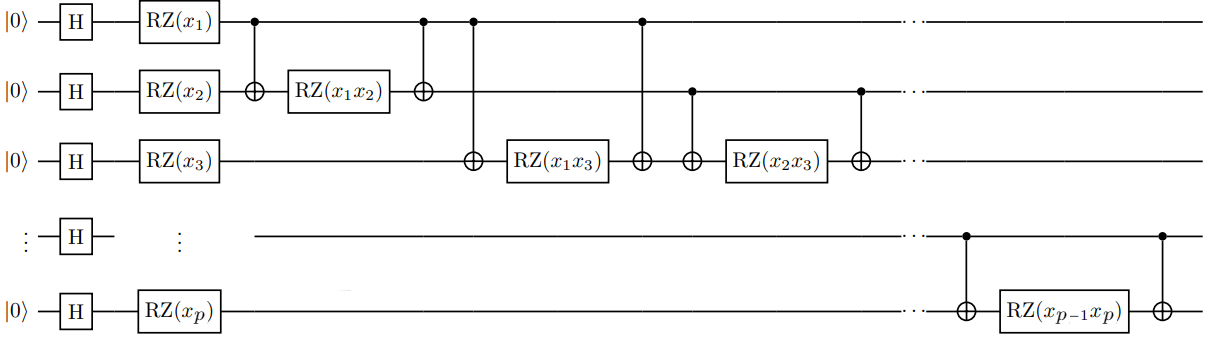
\includegraphics[width=14cm]{latex/figures/Rzz_encoding.png}
    \caption{Circuit visualizing implementation of RZZ encoding of $p$ features. The figure is retrieved from \cite{abbas2020power} and adapted to fit our notation.}
    \label{fig:Rzzencoding}
\end{figure}

This procedure produces a much more complex feature map, and can be made more complex still by repeating the whole encoding process several times in a row. The number of such repetitions is often called the \emph{depth} of the feature map.  \citet{abbas2020power} conjecture that this feature map is difficult to simulate classically for depth $\geq 2$ and increasing number of features. Since it requires $\mathcal{O}(p^2)$ operations on a quantum computer, its time complexity is polynomial and hence comparatively efficient. It was shown by the same authors that RZZ encoding produces much more flexible models than qubit encoding. However, it is also more computationally demanding, as it requires a circuit depth $\mathcal{O}(p^2)$ and full connectivity between all the qubits.

%================================================================
\subsection{Latent Qubits}\label{sec:Latent Qubits}
%================================================================
For both qubit encoding and RZZ encoding, the number of qubits in the circuit is restricted to be equal the number of features $p$ that is being encoded. This constrained can be relaxed by introducing \emph{latent qubits}, which are additional qubits added to the circuit that no features are encoded onto. This technique was originally proposed by (kilde), and was implemented to increase the size of Hilbert space for the same number of features. It is typical to apply a Hadamard gate to each latent qubit so that they don't start out in the $\ket{0}$ state. Subsequent ansatzes used for processing the data are then applied to all qubits, including the latent qubits. \autoref{fig:latent qubits} illustrate how latent qubits are added to a circuit. Here, $U_{\phi(\boldsymbol{x})}$ is any encoder, e.g. qubit encoding or RZZ encoding, that maps features on some number of qubits denoted $\ket{\boldsymbol{0}}$. Then, an arbitrary amount of qubits may be added to the circuit to increase the Hilbert space.

\begin{figure}[H]
         \centering
         \[\Qcircuit @C=1em @R=.7em {
         \lstick{\ket{\boldsymbol{0}}}& \gate{U_{\phi(\boldsymbol{x})}} &  \qw \\
         \lstick{\ket{0}}& \gate{H} &  \qw \\
         \vdots&  &   \\
         \lstick{\ket{0}}& \gate{H} &  \qw
         }\]
         \caption{Circuit encoding features expanded by adding an arbitrary number of latent qubits. Here, $U_{\phi(\boldsymbol{x})}$ is any encoder, e.g. qubit encoding or RZZ encoding, that maps features on some number of qubits denoted $\ket{\boldsymbol{0}}$. Then, an arbitrary amount of qubits may be added to the circuit to increase the Hilbert space.}
         \label{fig:latent qubits}
\end{figure}

%================================================================
%\subsection{Amplitude Encoding}\label{sec:AmplitudeEncoding}
%================================================================
%\emph{Amplitude encoding} is a way of encoding features directly as the amplitudes of a quantum state. Given a data set $\boldsymbol{x} = (x_1, \cdots, x_p)$, where $p=2^n$, amplitude encoding involves preparing a state $\ket{\psi_\boldsymbol{x}} = \sum_{i=1}^p x_i\ket{i}$ on $n$ qubits. Because of the normalization of quantum states, it is necessary to scale the data to ensure that $\sum_{i=1}^p |x_i|^2 = 1$ holds. The main advantage of amplitude encoding stems from the fact that the number of amplitudes is exponential in the number of qubit. Hence, we only need $\log_2(p)$ qubits to encode $p$ features, enabling us to encode an exponential amount of information as the number of qubits increase. However, there is not a general way of preparing a state for any given $\boldsymbol{x} = (x_1, \cdots, x_p)$ in an efficient way, i.e. with time-complexity polynomial in the number of qubits.

%Here, we will present a method for preparing an arbitrary state $\ket{\psi}$ with real-valued amplitudes starting from the initial state $\ket{0}$. The method is based on the description of \cite{SupervisedwquantumComputers}, which is in turn based on the work of \cite{Mottonen}. The method prepares the state by iterativly \emph{branching} the state by using multi-controlled rotations. Consider a general system of $n$ qubits. Starting in the state $\ket{00\cdots0}$ the algorithm applies an $R_y$ rotation with rotation angle $\beta^1_1$ on the first qubit
%\begin{equation}
%    \ket{\psi_1} = R_y^1(\beta^1_1)\ket{000} = a_1\ket{00\cdots0} + a_2\ket{10\cdots0},
%\end{equation}
%where the superscript of the gate indicates which qubit it acts on. 
%This creates two different branches where the first qubit is in state $\ket{0}$ and $\ket{1}$, respectively. Then, for each branch, we apply a different rotation on the second qubit. This can be done by conditioning the rotation on the first qubit, resulting in  
%\begin{equation}
%\begin{aligned}
%    \ket{\psi_2} = R_y^{2|q_1 = 0}(\beta^2_1)R_y^{2|q_1 = 1}(\beta^2_2)\ket{\psi_1} =\\ a_1(b_1\ket{00\cdots0} + b_2\ket{01\cdots0}) + a_2(b_3\ket{10\cdots0} + b_4\ket{11\cdots0}).
%\end{aligned}
%\end{equation}
%Here, the superscript "$2|q_1=0$" means that the gate is applied on the second qubit, conditioned on the first qubit being in state $\ket{0}$ ($q_1=0$). 
%In this way, each branch is broken into two new branches. This procedure is continued until all possible branches has been created. In general, we use multi-controlled rotations on qubit $i$ conditioned on all possible states of the preceding qubits, i.e.
%\begin{equation}
%    R_y^{i|q_1,\cdots,q_{i-1}}(\beta^i_j)\ket{q_1 \cdots q_{i-1}}\otimes \ket{0},
%\end{equation}
%where $j$ enumerates the $2^{i-1}$ different branches of $\ket{q_1 \cdots q_{i-1}}$. To ensure that we arrive at the desired amplitude after all the branches have been created, we must choose rotation angles

%\begin{equation}
%    \beta^{i}_j = 2\arcsin{
%    \frac{\sqrt{\sum_{l=1}^{2^{n-i}} |x_{(2j - %1)2^{n-i} + l}|^2}}
%    {\sqrt{\sum_{l=1}^{2^{n-i+1}} |x_{(j-1)2^{n-i+1}  %+ l}|^2}}
%    },
%\end{equation}
%with the special case for $i=n$

%\begin{equation}
%    \beta^{n}_j = 2\arcsin{
%    \frac{x_{(2j - 1) + l}}
%    {\sqrt{\sum_{l=1}^{2} |x_{2(j-1)  + l}|^2}}
%    }.
%\end{equation}
%As an easy example, lets say we want to encode the normalized features $\boldsymbol{x} = %(x_1, x_2, x_3 ,x_4)$ onto two qubits. We start by calculating the first rotation angle:
%\begin{equation}
%    \beta^{(1)}_1 = 2\arcsin{
%    \frac{\sqrt{|x_3|^2 + |x_4|^2}}{\sqrt{|x_1|^2 + |x_2|^2 + |x_3|^2 + |x_4|^2}}
%    } = 2\arcsin{\sqrt{|x_3|^2 + |x_4|^2}},
%\end{equation}
%where the normalization of the vector was used to remove the denominator. 

%The full procedure is visualized in the following circuit:

%\begin{equation}
%   \Qcircuit @C=1em @R=.7em {
%         \lstick{\ket{0}}& \gate{R_y(\beta^{1}_1)}&  \ctrl{1}                  & \ctrlo{1}                 & \qw &  \qw    &  \ctrl{1}                 & \ctrlo{1}                 &  \qw    &  \ctrlo{1}                        &\\
%         \lstick{\ket{0}}& \qw                      &  \gate{R_y(\beta^{2}_1)} & \gate{R_y(\beta^{2}_2)} & \qw &  \qw    &  \ctrl{2}                 & \ctrl{2}                  &  \qw    &  \ctrlo{2}                        &\\
%         \vdots          &                          &                            &                           &     &  \cdots &                           &                           &  \cdots &                                   &\\
%         \lstick{\ket{0}}& \qw                      &  \qw                       & \qw                       & \qw &  \qw    &  \ctrl{1}                 & \ctrl{1}                  &  \qw    &  \ctrlo{1}                        &\\
%         \lstick{\ket{0}}& \qw                      &  \qw                       & \qw                       & \qw &  \qw    &  \gate{R_y(\beta^{n}_1)}& \gate{R_y(\beta^{n}_2)} &  \qw    &  \gate{R_y(\beta^{n}_{2^{n-1}})} &\\
%         }        
%\end{equation}



    


%================================================================
\section{Ansatz}\label{sec:Ansätze}
%================================================================
What kinds of unitary transformation are interesting as ansätze used for processing information embedded in quantum states? In principle, we are able to explore every conceivable unitary transformation as a parameterized circuit, since there are circuit designs that are known to be \emph{universal}\cite{lloyd2018quantum}. In this context, universality means that for any unitary operator, there exists a sufficiently deep ansatz that approximates the operator to an arbitrary accuracy. However, such approximations are often exponentially deep\cite{NielsenQuantum}, meaning the vast majority of unitary transformations are inaccessible on ideal quantum computers, let alone near-term quantum computers. Still, it is believed that there exist reasonably shallow ansatz that are useful for constructing powerful machine learning models. Many of these ansätze are also believed to be classically hard to simulate, eluding to a possible quantum advantage for quantum machine learning\cite{lloyd2020quantum}.

In this thesis, we will investigate an ansatz that respect limitations of near-team quantum computers, constrained to circuit depth that scales linearly with the number of qubits and linear connectivity between qubits. We will refer to this ansatz as the \emph{simple ansatz}(SA). It can be visualised as 

\begin{equation}
U_{SA}(\boldsymbol{\theta}) = 
\begin{array}{c}
\Qcircuit @C=1.5em @R=.7em {
        &       \ctrl{1} & \qw       &  \qw      &  \qw      & \gate{R_y(\theta_1)}&\\
        &       \targ    & \ctrl{1}  &  \qw      &  \qw      & \gate{R_y(\theta_2)}&\\
        &       \qw      & \targ     &  \ctrl{0} &  \qw      & \gate{R_y(\theta_3)}&\\
        &       \vdots   &  \vdots         &  \vdots   &\vdots   & \vdots  \\
        &       \qw      & \qw       &  \qw      &  \targ    &\gate{R_y(\theta_{n_{\theta}})}&  \\
         }
\end{array}.
\end{equation}
The simple ansatz applies CNOT gates on neighboring qubits in sequence until the final qubit is reached. This creates entanglement between the qubits and enables access to a larger space of transformations, as explained in \autoref{sec:ControlledOperations}. Then, an $R_y$ rotation is applied to each qubit, each parameterized with its own parameter. Both the number of parameters and the circuit depth of the simple ansatz scales linearly with the number of qubits, making it hardware-efficient and hopefully suitable for near-term applications. 

In order to produce a more expressive ansatz, we may repeat the simple ansatz $d$ number of times with independent parameter as such:

\begin{equation}\label{eq:simple ansatz}
    \ket{\psi_{\boldsymbol{x}, \boldsymbol{\theta}}} = 
    U_{SA}(\boldsymbol{\theta}^r)\cdots U_{SA}(\boldsymbol{\theta}^2) U_{SA}(\boldsymbol{\theta}^1)\ket{\psi_{\boldsymbol{x}}},
\end{equation}
where $\boldsymbol{\theta}^i$ are independent vectors of parameters. We call $d$ the repetitions of the ansatz.

%================================================================
\section{Inference}\label{sec:Inference}
%================================================================
To derive a model output $\hat{y}$, we must estimate the expectation value of some observable with respect to the state prepared by the encoder and ansatz, i.e. $\hat{y} =\bra{\psi_{\boldsymbol{x},\boldsymbol{\theta}}}
\hat{O} 
\ket{\psi_{\boldsymbol{x},\boldsymbol{\theta}}}$. In the same manner as \cite{abbas2020power}, we use the \emph{parity} of the state to derive a model output for inference. The parity of an $n$ qubit state can be formulated as an operator as
\begin{equation}
    P = \frac{1}{2}(I^{\otimes n} + \bigotimes_{i=1}^n \sigma_z).
\end{equation}
Applying this operator on a computational basis state $\ket{v_1  \cdots v_n}$ computes 


\begin{equation}
    P\ket{v_1  \cdots v_n} = 
    \frac{1}{2}(\ket{v_1  \cdots v_n} -(-1)^{\sum_{i=1}^n v_i}\ket{v_1  \cdots v_2}) = 
    \bigoplus_{i=1}^n v_i \ket{v_1  \cdots v_n}, 
\end{equation}
where $\bigoplus_{i=1}^n v_i$ is the mod 2 sum of the terms $v_i$, also known as the parity of the bitstring $v_1\cdots v_n$. In short, the parity of the state is $0$ if the number of qubits in state $\ket{1}$ is even, and is otherwise 1. This is called even and odd parity, respectively. 

To estimate the expected parity $\bra{\psi_{\boldsymbol{x},\boldsymbol{\theta}}}P 
\ket{\psi_{\boldsymbol{x},\boldsymbol{\theta}}}$, we use the technique described in \autoref{sec:EstimatingExpectationValues} by preparing the state repeatedly and measure it in the computational basis. The expected parity can then be estimated as 

\begin{equation}
    \bra{\psi_{\boldsymbol{x},\boldsymbol{\theta}}}P 
    \ket{\psi_{\boldsymbol{x},\boldsymbol{\theta}}}
    \approx
    \frac{1}{S} \sum_{j=1}^S p_j,
\end{equation}
where $S$ is the number of shots used, and $p_j$ is the parity resulting from measurement $j$.


%================================================================
\section{Optimization of PQC}\label{sec:OptPQC}
%================================================================
A key component of hybrid methods such as PQC is the optimization of the parameters $\boldsymbol{\theta}$ entering the ansatz. These parameters are usually optimized with respect to some objective function in order to solve a given problem \cite{Benedetti_2019}. In the context of machine learning, one seeks to minimize the loss function \autoref{eq:LossFunction} to fit labeled data. There are multiple popular methods for optimization in the context of PQC. One such method is numerical differentiation of the loss function:

\begin{equation}
    \frac{\partial}{\partial \theta_i} L(\boldsymbol{\theta}) 
    \approx \frac{L(\theta_1, \cdots, \theta_i + \epsilon, \cdots \theta_{n_{\theta}}) - L(\theta_1, \cdots, \theta_i, \cdots \theta_{n_{\theta}})}{\epsilon},
\end{equation}
for a sufficiently small $\epsilon>0$. Having an approximation of the gradient, one can optimize the parameters using gradient descent or similar techniques. However, because of the high amount of noise of near-term quantum computers, finite difference approximations of derivatives can be unfavorable in practice. Recently, analytical techniques have been proved to be very efficient for calculating the gradient on quantum computers \cite{abbas2020power, Benedetti_2019}. In the next section, we will detail how this gradient can be calculated. 

%================================================================
\subsection{Analytical Gradient-Based Optimization}\label{sec:AnalyticalGrad}
%================================================================
Based on the derivation presented by \cite{Schuld_2019}, we will now present how the gradient of a large class of PQC's can be calculated on quantum computers using the \emph{parameter shift rule}.

Assume we have some circuit parameterized by $\boldsymbol{\theta}$ that prepares a state $\ket{\psi_{\boldsymbol{\theta}}} = U_{\boldsymbol{\theta}}\ket{0}$. The expectation value of some observable $\hat{O}$ can be formulated as 

\begin{equation}
    a = \bra{\psi_{\boldsymbol{\theta}}} \hat{O} \ket{\psi_{\boldsymbol{\theta}}} = \bra{0}U_{\boldsymbol{\theta}}^{\dagger}\hat{O}U_{\boldsymbol{\theta}}\ket{0}.
\end{equation}
Assume for simplicity that any parameter $\theta_i$ affects only a single gate. Then, since any circuit can be decomposed into a sequence of gates, we can decompose the circuit as $U_{\boldsymbol{\theta}}\ket{0} = AG(\theta_i)B$, where $G$ is the only gate dependent on $\theta_i$, and $A$ and $B$ is the rest of the circuit. This allows us to rewrite the expectation value as 

\begin{equation}
    a = \bra{\psi'} G(\theta_i)^{\dagger} \hat{O}' G(\theta_i) \ket{\psi'},
\end{equation}
where $\ket{\psi'} = B\ket{0}$ and $\hat{O}' = A^{\dagger}\hat{O}A$. Starting from this expression, it is easy to compute the derivative of the expectation value:

\begin{equation}
    \partial_{\theta_i} a = \bra{\psi'} G(\theta_i)^{\dagger} \hat{O}' (\partial_{\theta_i}G(\theta_i)) \ket{\psi'} + h.c.,
\end{equation}
where h.c. refers to the hermitian conjugate. In its current form, the terms of above expression cannot be computed on a quantum computer since they don't have the form of expectation values. However, it is possible to rewrite it as a linear combination of two expectation values

\begin{equation}\label{eq:generalDeriv}
\begin{aligned}
    \partial_{\theta_i} a = 
    \frac{1}{4}(
    \bra{\psi'} [G(\theta_i)+2\partial_{\theta_i}G(\theta_i)]^{\dagger} \hat{O}' [G(\theta_i)+2\partial_{\theta_i}G(\theta_i)] \ket{\psi'} -\\
    \bra{\psi'} [G(\theta_i)-2\partial_{\theta_i}G(\theta_i)]^{\dagger} \hat{O}' [G(\theta_i)-2\partial_{\theta_i}G(\theta_i)] \ket{\psi'}).
\end{aligned}
\end{equation}

Are $[G(\theta_i)+2\partial_{\theta_i}G(\theta_i)]$ and $[G(\theta_i)-2\partial_{\theta_i}G(\theta_i)]$ unitary operators? In the case that they are not, it is not possible to implement them as circuits. However, for gates such as Pauli rotations, they turn out to be unitary up to a constant factor and actually quite easy to implement. Given that $G(\theta_i) = R_j(\theta_i) = e^{-i\theta_i \sigma_j/2}$, where $j \in [x,y,z]$, we have that 
\begin{equation}
    G(\theta_i)\pm2\partial_{\theta_i}G(\theta_i) = 
    \underset{\sqrt{2}G(\pm \frac{\pi}{2})}{\underbrace{(I \mp i\sigma_j)}}G(\theta_i) = 
    \sqrt{2}G(\theta_i \pm \frac{\pi}{2}),
\end{equation}
where the relation $R_j(a)R_j(b) = R_j(a+b)$ was used in the last step. Inserting this result back into \autoref{eq:generalDeriv}, we get the final expression 


\begin{equation}\label{eq:parameterShiftRule}
\begin{aligned}
    \partial_{\theta_i} a = 
    \frac{1}{2}(
    \bra{\psi'} G(\theta_i + \frac{\pi}{2})^{\dagger} \hat{O}' G(\theta_i + \frac{\pi}{2}) \ket{\psi'} -\\
    \bra{\psi'} G(\theta_i - \frac{\pi}{2}) \hat{O}' G(\theta_i - \frac{\pi}{2}) \ket{\psi'}).
\end{aligned}
\end{equation}

The form of the expression above reveals the origin of the name "parameter shift rule". To calculate the derivative of the expectation value of a circuit, one simply has to estimate this expectation value twice: Once with the corresponding parameter shifted by $\frac{\pi}{2}$, and once shifted by $-\frac{\pi}{2}$. The derivative is finally found by combining the two results in a linear combination. This is a efficient approach for computing the gradient, since the number of expectation values that needs to be estimated is proportional to the number of parameters.

For QNNs, the features $\boldsymbol{x}$ enter the state $\ket{\psi_{\boldsymbol{x},\boldsymbol{\theta}}}$ in the same way as the parameters $\boldsymbol{\theta}$ if qubit encoding is used(see \autoref{sec:QubitEncoding}), i.e. with Pauli rotations. In this case, the parameter shift rule can also be applied to calculate the derivative of the output with respect to the features, i.e. $\partial_{x_i}a$. This will be relevant later when we introduce models consisting of multiple circuits. 

%================================================================
\subsection{Barren Plateus in QNN Loss Landscape}\label{sec:BarrenPlateus}
%================================================================
While recent studies have shown several promising characteristics of QNNs, such as faster training and greater flexibility\cite{abbas2020power}, these studies have largely been focused on smaller systems and heuristic measures. As such, few scaling relations of QNNs have been rigorously proven. Recently, \citet{McClean_2018} established an important result connecting the magnitude of the gradient and observables for a large class of PQCs to the number of qubits. First, they point out that expectation values measured on a state $\ket{\psi_n}$ sampled uniformly from an n-qubit Hilbert space tend to concentrate around the its mean over the whole Hilbert space as the number of qubits increases. Mathematically, we can express this as

\begin{equation}
    \lim_{n\to\infty} V(\bra{\psi_n}\hat{O}\ket{\psi_n}) = 0,
\end{equation}
where $V()$ indicates the variance, and $\hat{O}$ is some observable. Also, this concentration occurs exponentially fast in n. From \autoref{sec:Ansätze}, we know that a PQC $U_{\boldsymbol{\theta}}$  in general can prepare any state $\ket{\psi_\boldsymbol{\theta}}$ only if it is exponentially deep. However, \citet{McClean_2018} showed that shallow PQC with polynomial depth was also susceptible for the same exponential concentration of observable. This effect is also worsening the deeper the circuit is. Further, they showed that the gradient of PQC has a mean around zero, i.e.

\begin{equation}
     E(\partial \theta_i \bra{\psi_{\boldsymbol{\theta}}}\hat{O}\ket{\psi_{\boldsymbol{\theta}}}) = 0.
\end{equation}

These two results show that the gradients of PQCs are concentrating around zero. In other words, as the depth and width of PQCs grow, they essentially approach a random circuit, leading to a concentration of outputs around the average output over all possible initialization. In addition, their gradients vanish exponentially fast.

The vanishing of PQCs gradient manifests itself as loss landscapes that are extremely flat in most of parameter space, reminiscent of the vanishing gradient phenomenon of classical neural networks as the depth increases\cite{shalevshwartz2017failures}. The exponential vanishing of the gradient means that exponentially many shots are required in order to obtain a sufficient signal-to-noise ratio, as explained in \autoref{sec:EstimatingExpectationValues}. This may render the training of larger QNN models intractable as the number of qubits is increased in order to handle harder learning problems.


%================================================================
\section{Quantum Circuit Network}\label{sec:Quantum Circuit Network}
%================================================================
In order to extend the QNN framework discussed so far, we will implement multi-circuit models that utilize several such QNNs. These models exhibit a network-like structure, consisting of layers of several circuits. The layers of circuits transform feature vectors in a sequential manner until a model prediction is obtained. To avoid confusion with the similarly themed "quantum neural networks", we have opted to call the multi-circuit model a \emph{quantum circuit network}(QCN). This type of architecture was explored by \citet{b} and found able to sufficiently fit a nonlinear function in one dimension when optimized with Nelder-Meads algorithm, a gradient-free optimization algorithm.


%================================================================
\subsection{Feed-Forward}\label{sec:FeedForward}
%================================================================
\autoref{fig:QCN} illustrates the general structure of a quantum circuit network, which exhibits neural network-like architecture. Here, each node in the network is a QNN model $f^{(l)}_{QNN}$(see \autoref{eq:QNN}), with some layer specific choice of encoder, ansatz and observable. Each QNN is parameterized by $\boldsymbol{\theta}^{[l,j]}$, where $l$ is the layer and $j$ is the node in the current layer. The feed-forward procedure is described as follows: 
For layer $l$, each node receives the feature vector $\boldsymbol{a}^{(l-1)}$ resulting from the previous layer(with the special case that $\boldsymbol{a}^{(0)} = \boldsymbol{x}$). For each node $j$, an output $a^{(l)}_k$ is produced, i.e.
\begin{equation}
    a^{(l)}_j = f^{(l)}_{QNN}(\boldsymbol{a}^{(l-1)}; \boldsymbol{\theta}^{[l,j]})
\end{equation}
These outputs are then concatenated to make a new feature vector $\boldsymbol{a}^{(l)}$. This is then repeated for each layer $1$ through $L$. Finally, the output of the last is identified as the model output
\begin{equation}\label{eq:QCN}
    \hat{y} = f_{QCN}(\boldsymbol{x}; \boldsymbol{\theta}) = \boldsymbol{a}^{(L)},
\end{equation}
where $\boldsymbol{\theta}$ is the collection of all $\boldsymbol{\theta}^{[l,j]}$.


\begin{figure}[htp]
    \centering
    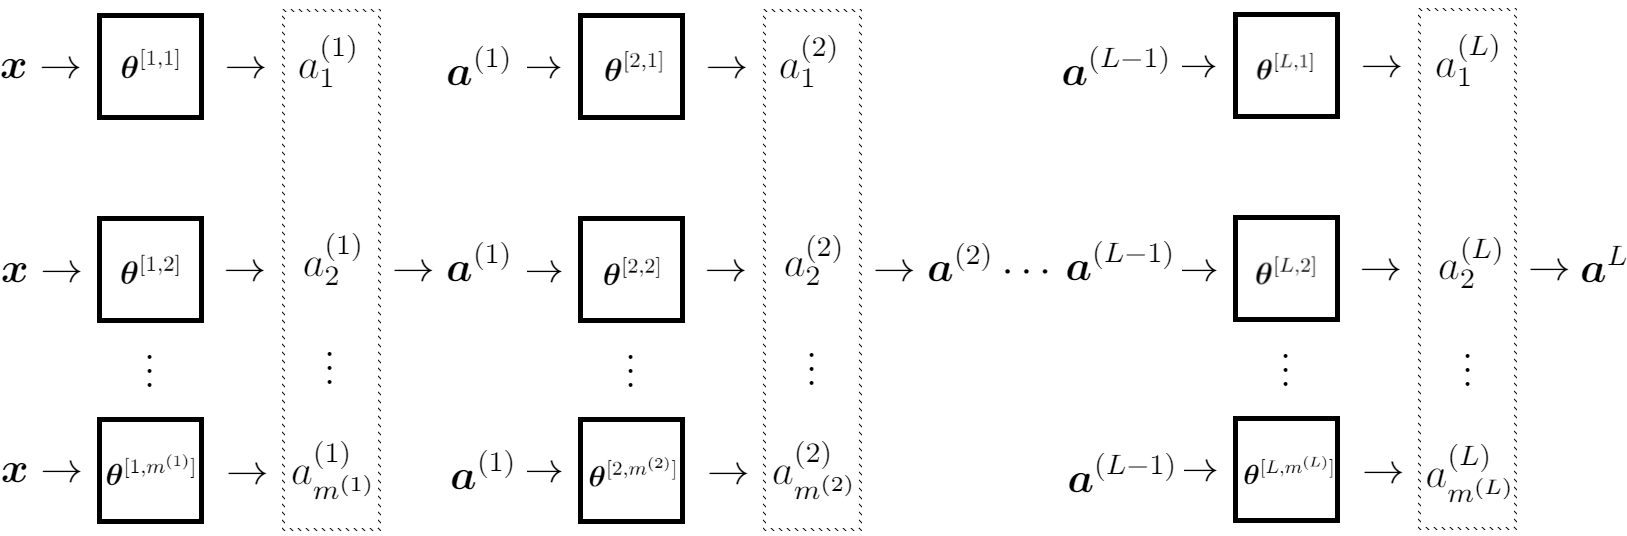
\includegraphics[width = 15cm]{latex/figures/QCN.png}
    \caption{General structure of a quantum circuit network. Each node, indicated by a box, is a QNN model parameterized by $\boldsymbol{\theta}^{[l,j]}$, where $l$ is the layer and $j$ is the node in the current layer. $m^{(l)}$ is the number of nodes in layer $l$. For layer $l$, each node receives the feature vector $\boldsymbol{a}^{(l-1)}$ resulting from the previous layer(with the special case that $\boldsymbol{a}^{(0)} = \boldsymbol{x}$). For each node $j$, an output $a^{(l)}_j$ is produced, which is then concatenated to make a new feature vector $\boldsymbol{a}^{(l)}$. This is then repeated for each layer $1$ through $L$. Finally, the output of the last layer is identified as the model output $\hat{y} = \boldsymbol{a}^{(L)}$.}
    \label{fig:QCN}
\end{figure}

The sequential transformation resulting from the multi-circuit architecture of QCNs offer several interesting properties compared to single circuit QNN models. The circuits can be evaluated one at a time and the output stored classically. This makes it possible to compute very large models of many parameters without the need for doing a long coherent computation on a quantum computer. While QNNs of many parameters must have either high circuits depths and or consist of many qubits (or both), QCN can on the other hand consist of many more shallow circuits of few qubits, much more suitable for near-term quantum computers. 

Further, the repeated encoding and estimation of outputs of intermediate layers introduce nonlinearities to the transformation of the data multiple times may alter the space of functions possible to compute in an interesting way. This is because each of these steps introduce a nonlinear transformation of the data. For classical neural networks, we know from \autoref{sec:DenseNeuralNetwork} that repeated nonlinear transformation is key for their great expressive power. Switching over to the single-circuit QNN model, nonlinearity is introduced only twice: First when the features are encoded as a quantum state using rotations such as $R_j(x_i)\ket{0} = \cos(\frac{x_i}{2})\ket{0} - i\sin(\frac{x_i}{2})\sigma_j\ket{0}$. The second time is when an output is derived by estimating an expectation value, which relates to the modulo square of the amplitudes of the state, i.e. $|\alpha_k|^2$. All other processing of the data is performed by the ansatz, which by definition is unitary and therefore linear in nature. In this sense, it could be that the formulation of QNNs as shown in \autoref{fig:QNN} could be a bit constrained with respect to what functions it can compute. By combining several circuits, nonlinearity is introduced with each layer, possibly creating a more powerful model able to fit more complicated functions.  



%================================================================
\subsection{Backward Propagation}\label{sec:BackwardPropagationQCN}
%================================================================
When comparing the formulation of QCN \autoref{eq:QCN} and classical neural network \autoref{eq:DNN}, it becomes apparent that they are structurally identical, excluding the mathematical operations happening inside each node. For the QCN, each node implements a QNN model, while the classical neural network implements an affine transformation, followed by a nonlinear activation. Using this observation, it is possible to implement a slightly modified backpropagation algorithm, earlier described in \autoref{sec:BackpropogationDNN}, for QCN. This assumes that we are able to calculate the derivative of the outputs of each QNN model. As described in \autoref{sec:ParametricModels}, this is indeed possible using the parameter shift rule. 

For $\hat{y} = f_{QCN}(\boldsymbol{x}; \boldsymbol{\theta})$ and a loss function $L(\hat{y}, y)$, the error of the last layer can be computed as 
\begin{equation}\label{eq:lastLayerErrorQCN}
    \delta^L_k = \frac{\partial L(\hat{y}, y)}{\partial \boldsymbol{a}^L_k},
\end{equation}
where $k$ indicates the node. This error can be defined for any layer recursively by repeated application of the chain-rule:
\begin{equation}\label{eq:errorQCN}
    \delta^l_j = \frac{\partial L(\hat{y}, y)}{\partial \boldsymbol{a}^l_j} 
    = \sum_k \frac{\partial L(\hat{y}, y)}{\partial \boldsymbol{a}^{l+1}_k} \frac{\partial \boldsymbol{a}^{l+1}_k}{\partial \boldsymbol{a}^{l}_j}
    = \sum_k \delta^{l+1}_k \frac{\partial \boldsymbol{a}^{l+1}_k}{\partial \boldsymbol{a}^{l}_j}.
\end{equation}

The derivative of the loss function with respect to any parameter in any node can then be calculated as 
\begin{equation}\label{eq:derivweightsQCN}
    \frac{\partial L(\hat{y}, y)}{\partial \theta^{[l,j]}_n} = 
    \sum_k \frac{\partial L(\hat{y}, y)}{\partial \boldsymbol{a}^{l}_k} \frac{\partial \boldsymbol{a}^{l}_k}{\partial \theta^{[l,j]}_n} 
    = \delta^l_j \frac{\partial \boldsymbol{a}^{l}_j}{\partial \theta^{[l,j]}_n},
\end{equation}
where it was used that $\frac{\partial \boldsymbol{a}^{l}_k}{\partial \theta^{[l,j]}_n} = 0$ for $k \neq j$, since the output of node $k$ is independent of the parameters in node $j$. 

The terms 
\begin{equation}\label{eq:localGradients}
\begin{aligned}
    \frac{\partial \boldsymbol{a}^{l}_j}{\partial \theta^{[l,j]}_n}, \frac{\partial \boldsymbol{a}^{l+1}_k}{\partial \boldsymbol{a}^{l}_j}
\end{aligned}
\end{equation} are the derivatives of the node outputs with respect to the parameters and inputs, respectively. Since they are calculated locally for each node, we call them the \emph{local gradients} of the QCN model. As explained in \autoref{sec:AnalyticalGrad}, the local gradients can be calculated analytically using the parameter shift rule with respect to the parameters $\theta^{[l,j]}_n$ and the inputs $\boldsymbol{a}^{l}_j$. By first performing a forward pass to calculate $\boldsymbol{a}^{l}$ for all the layers $l$, the local gradients can then be estimated and stored one at a time. Finally, \autoref{eq:derivweightsQCN} can be used to classically compute the \emph{total gradient} $\nabla_{\boldsymbol{\theta}} L(\hat{y},y)$ based on the stored values for the single sample $\boldsymbol{x}$. By repeating this for all samples $\boldsymbol{x}^{(i)}$, we can calculate the average total gradient \begin{equation}\label{eq:averageGradientQCN}
    \nabla_{\boldsymbol{\theta}} L(\boldsymbol{\theta}) = \frac{1}{N}\sum_{i=1}^N \nabla_{\boldsymbol{\theta}} L(\hat{y}^{(i)}, y^{(i)}).
\end{equation}  The calculation of the gradient allows us to leverage more information of the loss function and enables for gradient-based optimization. Potentially, this could mean faster optimization relative to derivative-free optimization, such as Nelder-Mead's algorithm which was originally used to optimize QCN(kilde). However, as explained in \autoref{sec:GradientDescent}, gradient-based methods such as gradient descent are prone to getting stuck in local minima, potentially causing slow optimization.    

%================================================================
%\subsection{Regularized Feature Map}\label{sec:Regularized Feature map}
%================================================================

%\begin{figure}[htp]
%\[ \begin{array}{c}
%    \Qcircuit @C=1em @R=1em {
%    \lstick{\ket{0}}& \multigate{3}{{U_{\phi(\boldsymbol{x})}}} & \qw    & %\multigate{3}{S_{\boldsymbol{\theta}}} & \qw    & %\multigate{3}{{U^{-1}_{\phi(\boldsymbol{x})}}} & \qw    &  \\
%    \lstick{\ket{0}}& \ghost{{U_{\phi(\boldsymbol{x})}}}        & \qw    & %\ghost{S_{\boldsymbol{\theta}}}        & \qw    %&\ghost{{U^{-1}_{\phi(\boldsymbol{x})}}}        & \qw    &  \\
%    \vdots          & \nghost{{U_{\phi(\boldsymbol{x})}}}       & \vdots & %\nghost{S_{\boldsymbol{\theta}}}       & \vdots & %\nghost{{U^{-1}_{\phi(\boldsymbol{x})}}}       & \vdots &   \\
%    \lstick{\ket{0}}& \ghost{{U_{\phi(\boldsymbol{x})}}}        & \qw    & %\ghost{S_{\boldsymbol{\theta}}}        & \qw    &\ghost{{U_{\phi(\boldsymbol{x})}}}    %    & \qw    &  \\
%                    & \underset{Encoder}{\underbrace{}}        &        %&\underset{Splitter}{\underbrace{}}    &        &\underset{Reverse  %Encoding}{\underbrace{}}        &             
%    }
%    \end{array}\]
%\caption{}
%\label{fig:QNN}
%\end{figure}



%================================================================
%\section{Recursive Circuit Optimization}\label{sec:RCO}
%================================================================

%Assume we have a unitary operator $U$ that prepares a state$\ket{\psi} = U\ket{0}$. In the case that $U$ has a high circuit depth, preparation of the state may fail on noisy hardware due to decoherence, as explained in \autoref{sec:Nisq}. 


%================================================================
\chapter{Tools for Analysis}\label{chap:TfA}
%================================================================
In this chapter, we introduce the various numerical methods used for investigating the models used in this thesis. 


%================================================================
\section{Trainability}\label{sec:Trainability}
%================================================================
In machine learning, \emph{trainability} refers to how easily a particular model can be trained under different conditions \cite{abbas2020power}. A common way of to asses the trainability is by assessing the geometry of the loss landscape. For example, the loss function of dense neural networks exhibit local flatness for most directions in parameter space, and strong distortion in others \cite{karakida2019universal}. In a loss landscape that is mostly flat, the gradient of the model tends to diminish, known as \emph{vanishing gradient}, making it difficult to train the model using gradient-based methods. This problem is known to worsen with the number of layers, making the training of deep models prohibitive.

To investigate the flatness and distortions of the loss landscape, a common metric to use is the \emph{Hessian} of the loss, which we will introduce in the next subsection. 
%================================================================
\subsection{Hessian Matrix}\label{sec:HessianMatrix}
%================================================================
Let $f(\boldsymbol{x}^{(k)}; \boldsymbol{\theta})$ be a parameterized and differentiable model, where $\boldsymbol{x}^{(k)} \in \mathbb{R}^p$ are $p$ features, and $\boldsymbol{\theta} \in \mathbb{R}^{n_\theta}$ are $n_{\theta}$ model parameters. For a general loss function on the form \autoref{eq:LossFunction}, $L(\boldsymbol{\theta}) = \sum{_{k=1}^{N}L(f(\boldsymbol{x}^{(k)};\boldsymbol{\theta}), y^{(k)}})$, where $N$ is the number of samples in the data set, the Hessian matrix of the loss function is given by

\begin{equation}
\label{eq:Hessian}
    H_{ij} = \frac{\partial^2 L(\boldsymbol{\theta})}{\partial \boldsymbol{\theta}_i\partial \boldsymbol{\theta}_j}.
\end{equation}

The Hessian matrix is an $n_\theta \times n_\theta$ matrix that quantifies the curvature of the loss function locally in the parameter space at the point of $\boldsymbol{\theta}$. This is an extensively studied quantity in the machine learning community, and it has been used to study the loss landscape both for classical and quantum mechanical machine learning models \cite{LeCun2012, Huembeli_2021}. In particular, its eigenvalue spectrum quantifies the amount of curvature in various directions. Typically for classical neural networks, the spectrum is characterized by the presence of many eigenvalues near zero, with the exception of a few large ones(so-called "big killers")\cite{LeCun2012}. This indicate the that loss landscape is mostly flat, with large distortions in a few directions, which in turn causes slow optimization as discussed earlier. 

%================================================================
\subsection{Empirical Fisher Information Matrix}\label{sec:EFIM}
%================================================================
An apparent shortcoming of the Hessian matrix \autoref{eq:Hessian} is the large computational cost of computing it, requiring the evaluation of $\mathcal{O}(n_\theta^2)$ double derivatives. This is particularly expensive for models of many parameters, which e.g. neural networks tend to be. An alternative and related quantity, called the \emph{Empirical Fisher Information Matrix}(EFIM)\cite{karakida2019universal}, can be calculated using $\mathcal{O}(n_\theta)$ first order derivatives, which is much better suited for big models. We will now derive the EFIM and relate it to the Hessian matrix.

Assume a square loss $\frac{1}{2N}\sum_{k=1}^{N} (f(\boldsymbol{x}^{(k)}; \boldsymbol{\theta}) - y^{(k)})^2$. Computing \autoref{eq:Hessian} with this loss results in 
    
\begin{equation}\label{eq:HessianSquareLoss}
    H_{ij} = F_{ij} -
    \frac{1}{N}\sum_{k=1}^{N} (y^{(k)} - f(\boldsymbol{x}^{(k)};\boldsymbol{\theta}))\frac{\partial^2 f(\boldsymbol{x}^{(k)};\boldsymbol{\theta})}{\partial \boldsymbol{\theta}_i\partial \boldsymbol{\theta}_j}, 
\end{equation}
where F is identified as the EFIM, given by
\begin{equation}
\label{eq:EmpiricalFisher}
    F_{ij} =  \frac{1}{N}\sum_{k=1}^{N}
    \frac{\partial f(\boldsymbol{x}_k;\boldsymbol{\theta})}{\partial \boldsymbol{\theta}_i}
    \frac{\partial f(\boldsymbol{x}_k;\boldsymbol{\theta})}{\partial \boldsymbol{\theta}_j}.
\end{equation}

From \autoref{eq:HessianSquareLoss}, the EFIM can been seen to coincide with the Hessian matrix if $f(\boldsymbol{x}^{(k)};\boldsymbol{\theta}) = y^{(k)}$, since the terms in the last sum vanishes. This is the case if the model manages to perfectly replicate the targets from the inputs, which is approximately true for well-trained models that fit the data sufficiently. However, even for untrained models, the EFIM is sometimes used as a cheaper alternative to the Hessian matrix, particularly for investigating the geometry of the loss landscape via its eigenvalue spectrum. This has been done both for classical and quantum mechanical machine learning models \cite{karakida2019universal} \cite{abbas2020power}. It is worth pointing out that these investigations, as well as this thesis, are mainly concerned with untrained models. Consequently, the EFIM does not coincide with the Hessian matrix and does not give a mathematically accurate description of the curvature of the loss landscape. However, the EFIM still serves as a heuristic for addressing the flatness and distortions of the loss landscape. 

%================================================================
\section{Expressivity}\label{sec:Expressivity}
%================================================================
\emph{Expressivity} in machine learning, especially in the context of neural networks, is a way of characterizing how architectural properties of a model affect the space of functions it can compute \citet{raghu2017expressive}. More simply put, expressivity measures how flexible and complex the model is. The first attempts to measure expressivity of neural networks took a highly theoretical approach, such as \citet{Bartlett} calculating of the VC dimension of shallow neural networks. The VC dimension, or \emph{Vapnik–Chervonenkis} dimension\cite{hastie01statisticallearning}, is a well-established measure of complexity. However, it is known to be hard to compute in practice for a variety of models\cite{abbas2020power}.  

%================================================================
\subsection{Trajectory Length}\label{sec:TrajectoryLength}
%================================================================
In order to assess the expressivity of deep neural networks, \citet{raghu2017expressive} introduced a more practical alternative to VC dimension called \emph{trajectory length}. This is an easy-to-compute heuristic that measures how small perturbations in the input of neural networks grows as it is passed through the various layers of the model. 

Given a trajectory $\boldsymbol{x}(t)$ in a $p$-dimensional space, its arc length 
$l(\boldsymbol{x}(t))$ is given by
\begin{equation}
   l(\boldsymbol{x}(t)) = 
   \int_{t} \big\Vert \frac{\boldsymbol{x}(t)}{dt} \big\Vert dt
\end{equation}
where $\Vert \cdot\Vert$ indicates the Euclidean norm. Conceptually, the arc length of the trajectory $\boldsymbol{x}(t)$ is sum of the norm of its infinitesimal segments. By approximating the trajectory with a finite number of points $\boldsymbol{x}(t_i)$, its arc length can be estimated as 

\begin{equation}\label{eq:TrajectoryLengthDiscrete}
   l(\boldsymbol{x}(t)) \approx 
   \sum_{i=1}^{N-1} \Vert\boldsymbol{x}(t_{i+1}) - \boldsymbol{x}(t_{i})\Vert.
\end{equation}

By making an appropriate trajectory $\boldsymbol{x}(t_i)$ in some input space, it is possible to investigate how its length changes as it is passed through each layer of a neural network. To be concrete, the quantity of interest is $l(\boldsymbol{a}^{l}(t_i))$, where $\boldsymbol{a}^{l}(t_i)$ are the outputs of layer $l$ resulting from the input $\boldsymbol{x}(t_i)$ for some neural network. As an example, one can make a trajectory $\boldsymbol{x}(t_i) \in \mathbb{R}^2$ in the shape of a circle. By projecting $\boldsymbol{a}^{l}(t_i)$ down to 2D, it is possible to visualize how each layer of the neural network distorts the trajectory. This has been exemplified in \autoref{fig:trajectoryLengthExample}.

\begin{figure}[H]
    \centering
    
\includegraphics[width=10cm]{latex/figures/trajectoryLengthExample.PNG}
    \caption{Figure showing a trajectory increasing with the depth
of a network. Starting with a circular trajectory (left most
pane), it is fed through a fully connected tanh network with
width 100. Pane second from left shows the image of the circular
trajectory (projected down to two dimensions) after being transformed by the first hidden layer. Subsequent panes show the trajectory after being transformed by multiple layers. This figure is retrieved from \citet{raghu2017expressive}.}
\label{fig:trajectoryLengthExample}
\end{figure}

\autoref{fig:trajectoryLengthExample} shows that the inputs gets transformed in a highly non-linear way as it is being transformed by each layer. Especially, neighboring points in the input trajectory gets mapped further and further apart for each transformation, indicating that small perturbations in the input grows for each layer. \citet{raghu2017expressive} showed that the trajectory length of trained neural networks increase exponentially with depth, suggesting a capacity to compute exponentially complex functions as the number of layers increase.




%==========================================================
%------- part 2: methodology & computational approach -----
%==========================================================
\part{Implementation}
%-------------------- placeholder --------------------
%================================================================
\chapter{Implementation}\label{chap:implementation}
%================================================================
In this chapter, we will present details surrounding implementation of algorithms and methods presented in \autoref{part:Theory}. For this thesis, we have developed an elaborate frame work for doing machine learning, capable of implementing dense neural networks(DNN, \autoref{eq:DNN}) and quantum circuit networks(QCN, \autoref{eq:QCN}). In addition, various numerical tools for analysing the models are available. The code base is object-orientated using Python, focusing on flexibility. This grants huge freedom when specifying model architecture, such as setting the number of layers, number of nodes, type of activation functions, loss function and optimizer. The frame work is also capable of implementing hybrid models mixing both DNN and QNC layers. To implement quantum machine learning, the frame work is built around Qiskit\cite{Qiskit}, an IBM-made python-package used for emulating quantum circuits. 

All source code developed for this thesis can be found on our GitHub page \url{https://github.com/KristianWold/Master-Thesis}, together with notebooks containing training of models, generation of data, analysis and plotting. For easier reading, all python types referred to in this thesis will be highlighted in \textbf{bold}.

%================================================================
\section{Qiskit}\label{sec:Qiskit}
%================================================================

Qiskit\cite{Qiskit} is an open source python-package used for practically emulating quantum circuits and quantum algorithms. It can be installed using pip with the following command:

\begin{lstlisting}[language=bash]
  $ pip install qiskit
\end{lstlisting}
To import the package, include the following among the import in any python scrip:
\begin{lstlisting}[language=python]
  import qiskit as qk
\end{lstlisting}

%================================================================
\subsection{Registers and Circuits}\label{sec:QMLE}
%================================================================

To create a quantum circuit in Qiskit, one can first create one or more \emph{quantum registers}, which are list structures containing qubits. The registers can be put together into a circuit in the following way:

\begin{lstlisting}[language=python, numbers=left]
q_reg_1 = qk.QuantumRegister(2)
q_reg_2 = qk.QuantumRegister(2)
c_reg = qk.ClassicalRegister(2)
circuit = qk.QuantumCircuit(q_reg_1, q_reg_2, c_reg)
\end{lstlisting}
Here, each of the registers \textbf{q\_reg\_1} and \textbf{q\_reg\_2} contains two qubits. By default, they are each initialized in the state $\ket{0}$. Thus, total circuit can be written as
\begin{equation}
    \ket{00}\ket{00},
\end{equation}
where is \emph{ket} refers to one register. Further, \textbf{c\_reg} is a \emph{classical register} of classical bits, meant for storing classical information when the circuit is later measured. In general, a circuit can contain any number of quantum registers with any number of qubits. However, if one wishes to include a classical register, it must be included as the last argument in \textbf{qk.QuantumCircuit()}.

%================================================================
\subsection{Applying Gates}\label{sec:operationsOnQubits}
%================================================================

Continuing after creating our circuit, we may apply a variety of quantum gates by calling different methods for the \textbf{circuit} object. Hadamard gates can be applied to the two qubits of register \textbf{q\_reg\_1} in the following way:

\begin{lstlisting}[language=python, numbers=left]
circuit.h(q_reg_1[0])
circuit.h(q_reg_1[1])
\end{lstlisting}

This prepares the state 
\begin{equation*}
    \ket{00}\ket{00} \rightarrow 
    \big(\frac{1}{2}\ket{00} + \frac{1}{2}\ket{01} +
    \frac{1}{2}\ket{10} + \frac{1}{2}\ket{11}\big)\ket{00}  
\end{equation*}


A possible way of creating entanglement between the registers is to use CNOT gates on \textbf{q\_reg\_2} conditioned on the qubits in \textbf{q\_reg\_1}:


\begin{lstlisting}[language=python, numbers=left]
circuit.cx(q_reg_1[0], q_reg_2[0])
circuit.cx(q_reg_1[1], q_reg_2[1])
\end{lstlisting}
resulting in the state 

\begin{equation*}
\begin{aligned}
\big(\frac{1}{2}\ket{00} + \frac{1}{2}\ket{01} +
\frac{1}{2}\ket{10} + \frac{1}{2}\ket{11}\big)\ket{00} \rightarrow \\
\frac{1}{2}\ket{00}\ket{00} + \frac{1}{2}\ket{01}\ket{01} +
\frac{1}{2}\ket{10}\ket{10} + \frac{1}{2}\ket{11}\ket{11}
\end{aligned}
\end{equation*}


For a complete documentation of the gates available in Qiskit, see \url{https://qiskit.org/documentation/stubs/qiskit.circuit.QuantumCircuit.html}.

%================================================================
\subsection{Measurement}\label{sec:MeasurementQiskit}
%================================================================

To measure the state of \textbf{q\_reg\_2} in the computational basis and store it to \textbf{c\_reg}, we make use of the method \textbf{measure()}:

\begin{lstlisting}[language=python, numbers=left]
  circuit.measure(q_reg_2, c_reg)
\end{lstlisting}

Finally, to repeatedly execute the circuit and sample the results, we make use of \textbf{qk.execute} together with the backend \emph{qasm\_simulator}:


\begin{lstlisting}[language=python, numbers=left]
job = qk.execute(circuit, 
                 backend = 
                 qk.Aer.get_backend("qasm_simulator"),
                 shots = 1000)
result = job.result().get_counts(circuit)
print(result)
\end{lstlisting}

\begin{flalign*}
    & \rightarrow \{'00':261, '01':242, '10':253, '11':244\} &
\end{flalign*}
Resulting from this is a python dictionary whose keys are strings indicating the different states that was measured. The value corresponding to each key is the number of times that state was measured. To set the number of times to execute and measure the circuit, the argument \textbf{shots} may be used. In this case, it was set to 1000. Using \textbf{qk.Aer.get\_backend("qasm\_simulator")} as the backend, the circuit is simulated locally on the classical machine in an ideal fashion, meaning the imperfections of real quantum computers as described in \autoref{sec:Nisq} are disregarded. Still, since a finite number of shots was used, the normalized results $\frac{261}{1000}$, $\frac{242}{1000}$, $\frac{253}{1000}$ and $\frac{244}{1000}$ only approximate the exact value $\frac{1}{4}$. 

%================================================================
\subsection{Exact Expectation Value}\label{sec:Exact Expectation Value}
%================================================================

When simulating circuits on classical hardware, e.g. with Qiskit, we have the luxury of being able to access state resulting from some computation directly and calculate exact expectation values. As explained in \autoref{sec:MeasuringState}, this is not possible when using real quantum computers. Have access to exact expectation values is useful when the noise of finite sampling or realistic hardware is uninteresting for the analysis. 

To access the exact state, the classical register \textbf{c\_reg} must be omitted from the circuit, as we never plan to measure it in the ordinary way. Then, the circuit is simulated using the \emph{statevector\_simulator} backend:

\begin{lstlisting}[language=python, numbers=left]
job = qk.execute(circuit, 
                 backend = 
                 qk.Aer.get_backend("statevector_simulator"))
result = job.result().get_counts(circuit)
print(result)
\end{lstlisting}
\begin{flalign*}
    & \rightarrow \{'00':0.25, '01':0.25, '10':0.25, '11':0.25\} &
\end{flalign*}
Here, the "measurements" are exact and normalized, as if infinitely many shots were used for sampling. 


%================================================================
\subsection{Simulating Real Devices}\label{sec:Simulating Real Devices}
%================================================================



%================================================================
\section{QNN Example}\label{sec:QNNimpement}
%================================================================
We will now present a possible way of implementing a QNN \autoref{eq:QNN} for fitting the popular Iris data set(kilde). The model will be optimized using the parameter shift rule and gradient descent. 

%================================================================
\subsection{Encoding}
%================================================================

To encode the data, we will make a callable object on the form \textbf{circuit = encoder(circuit, data\_reg, data)}, where \textbf{data\_reg} is a quantum register of \textbf{circuit}, and \textbf{data} is a numpy array containing the features of one sample. Qubit encoding using $R_x$ rotations, as presented in \autoref{sec:QubitEncoding}, can be implemented as the following function:

\begin{lstlisting}[language=python, numbers=left]
def qubit_encoder(circuit, data_reg, data):
    for i, x in enumerate(data):
        circuit.rx(x, data_register[i])
        
    return circuit
\end{lstlisting}

This function requires that the number of features does not exceed the number of qubits.

%================================================================
\subsection{Ansatz}
%================================================================
To implement the ansatz, we want a callable object on the form 
\textbf{circuit = ansatz(circuit, data\_reg, theta, reps)}, where \textbf{theta} is a numpy array containing the parameters. The "simple ansatz" detailed in \autoref{sec:Ansätze} can be implemented as a python function:

\begin{lstlisting}[language=python, numbers=left]
def simple_ansatz(circuit, data_reg, theta):
    n_qubits = data_reg.size()
    
    for i range(n_qubits - 1):
        circuit.cx(data_reg[i], data_reg[i+1])
    
    for i, w in enumerate(theta):
        circuit.ry(w, data_register[i])
        
    return circuit
\end{lstlisting}
Here, \textbf{data\_reg.size()} was used to retrieve the number of qubits present in the register. The first for-loop ensures to entangle the qubits in sequence using CNOT gates. The last for-loop applies an $R_y$ rotation to each qubit corresponding to the parameters.

%================================================================
\subsection{Inference}\label{sec:InferenceImplementation}
%================================================================
To derive an inference from the model, we must estimate an expectation value as explained in \autoref{sec:Inference}. We can do this by making a callable object \textbf{y\_pred = sampler(counts)}, where \textbf{counts} is a python dictionary containing the measuring results, as explained in \autoref{sec:MeasurementQiskit} and \autoref{sec:Exact Expectation Value}. We can implement a function estimating the parity(see \autoref{sec:Inference}) in the following way:

\begin{lstlisting}[language=python, numbers=left]
def parity(counts):
    shots = sum(counts.values())
    
    output = 0
    for bitstring, samples in counts.items():
        if parity_of_bitstring(bitstring) == 1:
            output += samples

    output = output / shots

    return output
\end{lstlisting}
where \textbf{parity\_of\_bitstring(bitstring)} is a function that calculates the parity of a bitstring, which can be implemented as 
\begin{lstlisting}[language=python, numbers=left]
def parity_of_bitstring(bitstring):
    binary = [int(i) for i in bitstring]
    parity = sum(binary) % 2
    
    return parity
\end{lstlisting}

The function \textbf{parity()} iterates over the different measured states and makes a weighted average of their parities, resulting in the estimation of the average parity of the state.

To performe the whole inference, we can implement a function \textbf{qnn(x, theta)}, where \textbf{x} is a numpy array containing features of a single sample, and \textbf{theta} is a numpy array containing parameters. The function can be implemented as 

\begin{lstlisting}[language=python, numbers=left]
def qnn(x, theta):
    n_qubits = len(x)
    reps = 2
    data_reg = qk.QuantumRegister(n_qubits)
    clas_reg = qk.ClassicalRegister(n_qubits)
    circuit = qk.QuantumCircuit(data_reg, clas_reg)
    
    circuit = qubit_encoder(circuit, data_reg, x)
    circuit = simple_ansatz(circuit, theta, reps)

    job = qk.execute(circuit, 
                     backend = 
                     qk.Aer.get_backend("qasm_simulator"),
                     shots = 1000)
    counts = job.result().get_counts(circuit)
    y_pred = parity(counts)
    
    return y_pred
\end{lstlisting}


%================================================================
\subsection{Gradient}\label{sec:GradientImplementation}
%================================================================
Having a function that implements a QNN that performs inference, we can apply the parameter shift rule described in \autoref{sec:AnalyticalGrad} to calculate the gradient of the output with respect to the parameters:

\begin{lstlisting}[language=python, numbers=left]
def gradient(x, theta):
    deriv_plus = np.zeros(len(theta))
    deriv_minus = np.zeros(len(theta))
    
    for i in range(len(theta)):
        theta[i] += np.pi/2 #parameter shifted forward
        deriv_plus[i] = qnn(x, theta) 
        
        theta[i] -= np.pi   #parameter shifted backwards
        deriv_minus[i] = qnn(x, theta)
        
        theta[i] += np.pi/2 #parameter reset
    
    return 0.5*(deriv_plus - deriv_minus) #linear combination
\end{lstlisting}
This function returns a numpy array with the same length as \textbf{theta}, containing the derivatives $\frac{\partial y}{\partial \theta_i}$.

%================================================================
\subsection{Training}\label{sec:QNNTraining}
%================================================================

Finally, we can implement a function \textbf{train(x\_list, y\_list, theta, lr, epochs)} that calculates the average gradient \autoref{eq:averageGradient} resulting from the samples and targets \textbf{x\_list} and \textbf{y\_list}, using MSE loss. The function then updates the parameters \textbf{theta} iterativly(\textbf{epochs} number of times) using gradient descent with learning rate \textbf{lr}:

\begin{lstlisting}[language=python, numbers=left]
def train(x_list, y_list, theta, lr, epochs):
    loss = []
    for i in range(epochs):
        grad = np.zeros(len(theta))
        loss.append(0)
        
        for x, y in zip(x_list, y_list):
            y_pred = qnn(x, theta)      #inference
            loss[-1] += (y_pred - y)**2 #accumulate loss        
            grad = grad + (y_pred - y)*gradient(x, theta)
        
        loss[-1] = loss[-1]/len(y)      #normalize
        grad = grad/len(y)
        theta += -lr*grad               #update parameters
    
    return theta, loss
\end{lstlisting}

At line 10, \textbf{grad += (y\_pred - y)*gradient(x, theta)} accumulates the gradient of the MSE loss function with respect to the parameter, i.e. \autoref{eq:LossDerivateWRTparameter}. The parameters are then updated at line 14.


%================================================================
\subsection{Putting It All Together}\label{sec:PIAT}
%================================================================
Stuff

%================================================================
\section{Quantum Circuit Network}\label{sec:QCNimplementation}
%================================================================
Stuff

%================================================================
\subsection{Encoders, Ansätze and Samplers}\label{sec:EAaS}
%================================================================
In the QCN framework, we implement encoders, ansätze and samplers as callable python classes with much the same functionality as described in \autoref{sec:QNNimpement}. We will now go thorugh the use of the most important classes.

\subsubsection*{QubitEncoder}
The encoder class \textbf{QubitEncoder} can be instantiated as 

\begin{lstlisting}[language=python, numbers=left]
from encoders import QubitEncoder

encoder = QubitEncoder(mode)
\end{lstlisting}

Here, \textbf{mode} is a string that specifies the rotation used for encoding, either \textbf{"x"}, \textbf{"y"} or \textbf{"z"}. See \autoref{sec:QubitEncoding} for details.

\subsubsection*{Ansatz}
The ansatz class \textbf{Ansatz} can be instantiated as
\begin{lstlisting}[language=python, numbers=left]
from ansatzes import Ansatz

ansatz = Ansatz(block, reps)
\end{lstlisting}
Here, \textbf{block} is a python list containing strings that specify gates that are applied to the circuit. For example, 
\textbf{block = ["entangle", "ry"]} will first apply CNOT gates to all neighboring qubits in sequence. $R_y$ rotations are then applied to every qubit. This particular argument recreates the simple ansatz described in \autoref{sec:Ansätze}. \textbf{reps} specifies the number of times the ansatz is then repeated.

\subsubsection*{Parity}
The sampler class \textbf{Parity} can be instantiated as
\begin{lstlisting}[language=python, numbers=left]
from samplers import Parity

sampler = Parity()
\end{lstlisting}
This class implements the same functionality as the \textbf{parity} function described in \autoref{sec:QNNimpement}.

%================================================================
\subsection{QLayer}\label{sec:QLayer}
%================================================================

Our framework for making QCN models implements layers consisting of QNN models as nodes, as explained in \autoref{sec:Quantum Circuit Network}. In the framework, a QCN layer can be created as a python object of the type \textbf{QLayer} in the following way:

\begin{lstlisting}[language=python, numbers=left]
from layers import QLayer

qlayer = QLayer(n_qubits,   #number of qubits in each QNN
                n_features, #number of input features
                n_targets,  #number of outputs, i.e. nodes
                scale,      #scaling of output
                encoder,
                ansatz,
                sampler,
                backend,
                shots)
\end{lstlisting}

The arguments \textbf{encoder}, \textbf{ansatz} and \textbf{sampler} defines the architecture of each QNN in the layer. Examples of possible choices are described in \autoref{sec:EAaS}. 

As an example, a \textbf{QLayer} can be instantiated and used on a data in the following way:


\begin{lstlisting}[language=python, numbers=left]
import qiskit as qk
from layers import QLayer
backend = qk.Aer.get_backend("qasm_simulator")

x = np.random.normal((4,3))

qlayer = QLayer(n_qubits = 3,
                n_features = 3,
                n_targets = 2,
                scale = 2*np.pi,
                encoder = QubitEncoder(mode = "x"),
                ansatz = Ansatz(blocks=["entangle", "y"],
                reps = 2),
                sampler = Parity(),
                backend = backend,
                shots=1000)
                
y_pred = qlayer(x)
print(y_pred)
\end{lstlisting}
(skriv output her)

Here, \textbf{x} is a dataset containing four samples of three features each. By specifying \textbf{n\_targets=2}, the layer consists of two nodes and produces thus two output targets. The layer is callable, and performs inference on the input \textbf{x} sample-wise.

If the number of shots are set to zero, i.e. \textbf{shots=0}, the outputs are exactly calculated with the \emph{statevector\_simulator} backend, as explained in \autoref{sec:Exact Expectation Value}.

%================================================================
\subsection{Constructing QCNs from QLayers}\label{sec:ConstructingNetworks}
%================================================================
In general, a QCN can be constructed with any number of layers, with any number of inputs and outputs. The only constraint is that the outputs of one layer and the inputs of a subsequent layer must match in shape.

A two-layer QNC can be constructed in the following way using the \textbf{NeuralNetwork} class:

\begin{lstlisting}[language=python, numbers=left]
from neuralnetwork import NeuralNetwork

x = np.random.normal(0, 1, (4,3))

#unspecified arguments assumes default values
layer1 = QLayer(n_qubits=3,
                n_features=3,
                n_targets=4) 
                
layer2 = QLayer(n_qubits=4,
                n_features=4,
                n_targets=1)

network = NeuralNetwork(layers = [layer1, layer2],
                        cost = MSE(),
                        optimizer = Adam(lr=0.1))          
y_pred = network.predict(x)
print(y_pred)
\end{lstlisting}
 
In the above code, the \textbf{NeuralNetwork} class stores the layer objects in a python list \textbf{self.layers}. When doing inference, the class implements feed forward, as described in \autoref{sec:FeedForward}, using a \textbf{\_call\_} method:
\begin{lstlisting}[language=python, numbers=left]
def __call__(self, x):
        self.a = []
        self.a.append(x)
        for layer in self.layers:
            x = layer(x)
            self.a.append(x)
\end{lstlisting}
The output of all layers are stored, as they are needed during back-propagation. \textbf{network.predict(x)} returns only the output of the last layer, i.e. the model output. 

%================================================================
\subsection{Back Propagation}\label{sec:BackpropImplementation}
%================================================================

The class \textbf{NeuralNetwork} performs back propagation, as described in \autoref{sec:BackwardPropagationQCN}, using a class method \textbf{network.backward(x,y)}. In simplified terms, the method is implemented as:
\begin{lstlisting}[language=python, numbers=left]
def backward(self, x, y):
    self(x)                 #feed forward      
    y_pred = self.a[-1]     #inference
    delta = self.cost.derivative(y_pred, y)

    #work thru layers in reverse
    for i, layer in reversed(list(enumerate(self.layers))):
        weight_gradient, delta = layer.grad(self.a[i], 
                                            delta)
        self.weight_gradient_list.append(weight_gradient)

    self.weight_gradient_list.reverse()
\end{lstlisting}
\textbf{network.backward(x,y)} starts by performing feed forward and inference. In line 4, the error of the last layer \autoref{eq:lastLayerErrorQCN} is initiated as \textbf{delta}. For each layer, starting with the last first, the gradient is calculated and the error \textbf{delta} is updated. This is done using \autoref{eq:derivweightsQCN} and \autoref{eq:errorQCN}, respectively, which is implemented in the layer method \textbf{layer.grad(self.a[i], delta)}.

%================================================================
\subsection{Training}\label{sec:QCNTraining}
%================================================================
To train the QCN, the class method \textbf{network.train(self, x, y, epochs)} can be used. In simplified terms, it is implemented as

\begin{lstlisting}[language=python, numbers=left]
def train(self, x, y):
    self.loss = []
    for i in range(epochs):
        self.backward(x, y)
        self.step()

        y_pred = self.a[-1]
        self.loss.append(self.cost(y_pred, y))
            
    y_pred = self.predict(x)
    self.loss.append(self.cost(y_pred, y))
\end{lstlisting}
The method for training starts by calling \textbf{self.backward} in order to calculate and store the gradient in \textbf{self.weight\_gradient\_list}. Then, the method \textbf{self.step()} is used to update the parameters of the layers. This is done using \autoref{eq:ParameterUpdate}, but with the gradient modified by the specified optimizer. This is then repeated a number of times specified by \textbf{epochs}.

%================================================================
\subsection{Single-Circuit Models}\label{sec:Single-CircuitModel}
%================================================================
Using the \textbf{NeuralNetwork}, it is possible to construct single-circuit QNNs in addition to the usual multi-circuit QCNs. This can be done using a single \textbf{QLayer} with a single node, as this will constitute only one QNN:
\begin{lstlisting}[language=python, numbers=left]
layer = QLayer(n_qubits = 4,
               n_features = 4,
               n_targets = 1,
               encoder = RZZEncoder(),
               ansatz = Ansatz(blocks=["entangle", "ry"],
                               reps=2),
               sampler = Pairty(),
               backend = backend,
               shots = 1000)
                               

qnn_model = NeuralNetwork(layers = [layer1])
\end{lstlisting}
As there are no intermediate layers, we do not need to compute the derivative of the node outputs with respect to their inputs. This opens up for ways of encoding where the parameter shift rule, as implemented in \autoref{sec:AnalyticalGrad} and \autoref{sec:GradientImplementation}, fails. Possible choices is RZZ encoding(as used in the above code) and amplitude encoding.

%================================================================
\subsection{Hybrid Networks}\label{sec:Hybrid Networks}
%================================================================
In addition to \textbf{QLayer} layers, the neural network framework also implements \textbf{Dense} layers, which are densely connected, classical layers as defined in \autoref{sec:DenseNeuralNetwork}. It can be instantiated in the following way:

\begin{lstlisting}[language=python, numbers=left]
from layers import Dense, Sigmoid

dense = Dense(n_features = 4,
              n_targets = 3,
              scale = 1,
              activation = Sigmoid(),
              bias = True)
\end{lstlisting}
Here, \textbf{activation} specifies the activation of the layer, in this case the sigmoid function. Setting \textbf{bias} to true enables the use of bias parameters in the layer. Like \textbf{QLayer}, \textbf{Dense} also implements methods like \textbf{\_call\_} for feed forward, and \textbf{grad()} for back-propagation. This opens up for construction of neural networks that consists of an arbitrary combination of \textbf{QLayer} and \textbf{Dense} layers, which can be simultaneously optimized using the methods of \autoref{sec:QCNTraining}.

%================================================================
\section{Tools for Analysis}\label{sec:Tools for Analysis Imp}
%================================================================

%================================================================
\subsection{Magnitude of Gradient}\label{sec:Gradient Magnitude}
%================================================================



%================================================================
\subsection{Empirical Fisher Information}\label{sec:FIMImplement}
%================================================================
To investigate the loss landscape of the QCN model, we calculate the EFIM \autoref{eq:EmpiricalFisher} and its eigen value spectrum using a class \textbf{EFIM}. Given some \textbf{network} and data set \textbf{x}, it can be used in the following way:
\begin{lstlisting}[language=python, numbers=left]
from analysis import EFIM

efim = EFIM(network)
efim.fit(x)
\end{lstlisting}
Calling \textbf{efim.fit(x)} calculates the EFIM of \textbf{network} over the data \textbf{x}, and is impemented as
\begin{lstlisting}[language=python, numbers=left]
def fit(self, x):
    n_samples = x.shape[0]

    self.model.backward(x, samplewise=True)
    gradient = self.model.weight_gradient_list

    gradient_flattened = []
    for grad in gradient:
        gradient_flattened.append(grad.reshape(n_samples, -1))

    gradient_flattened = np.concatenate(gradient_flattened, axis=1)

    self.fim = 1 / n_samples * gradient_flattened.T @ gradient_flattened
\end{lstlisting}
At line 4, the cost function of the network is set to \textbf{NoCost()}. This ensures that \textbf{backward} calculates the gradient of the model output and not any particular loss, which is required by the EFIM. In addition, specifying \textbf{samplewise=True} in the \textbf{backward()} method stops the gradient from being averaged over all the samples. Rather, it is stored individually for each sample. The following for-loop unravels and concatenates all the gradients of the various layers into a single matrix with dimension $(N, n_{\theta})$, which is the number of samples and parameters, respectively. The EFIM is calculated as a matrix product in line $13$, normalized by the number of samples. This matrix is then stored in \textbf{self.efim}

After calculating the EFIM, its eigenvalue spectrum can be calculated as 

\begin{lstlisting}[language=python, numbers=left]
eigenvalue_spectrum = efim.eigen(x)
\end{lstlisting}
This performs a simple eigenvalue decomposition of \textbf{self.efim} using numpy's \textbf{linalg.eigh} to extract the eigenvalues. Because the EFIM is often very degenerate, some of the lower lying eigenvalues turn out negative, likely because of floating-point errors. To combat this, any eigenvalue lower than $10^{-25}$ is set to this value. 

%================================================================
\subsection{Trajectory Length}\label{sec:TrajectoryLengthImplement}
%================================================================
Assume we have a \textbf{NeuralNetwork} object and a trajectory $\boldsymbol{x}(t_i)$, as described in \autoref{sec:TrajectoryLength}. Then, we can calculate the trajectory length \autoref{eq:TrajectoryLengthDiscrete} of the resulting outputs of each layer using the class \textbf{TrajectoryLength}:

\begin{lstlisting}[language=python, numbers=left]
from analysis import TrajectoryLength

tl = TrajectoryLength(network)
traj_len, traj_proj = tl.fit(x)
\end{lstlisting}
This produces a two python list: \textbf{traj\_len} contains the trajectory length of the layer outputs. \textbf{traj\_proj} contains the layer outputs themselves, projected down onto 2D for visualization. The projection was done using scikit-learn's(kilde) PCA decomposition. (Describe code?)



























%==========================================================
%-------------- part 3: results & discussion --------------
%==========================================================

\part{Results \& Discussion}
%-------------------- placeholder --------------------
%================================================================
\chapter{Results and Discussion}\label{chap:results_discussion}
%================================================================
In this chapter, we will investigate and characterize models discussed in earlier chapters. We will also detail how the various models are configured, and how numerical methods are used for characterization. The results will be briefly commented as they are presented, with a more in-depth discussion at the end of each section.

In \autoref{sec:Vanishing Gradient Phenomenon}, we investigate and compare the vanishing gradient phenomenon for QNNs, QCNs and DNNs by studying how the magnitude of their gradients vary as a function of architecture. There will be put emphasis on the behaviour with respect to the number of layers.

In \autoref{sec:Investigating the Loss Landscape}, we will characterize the geometry of the loss landscape of QNNs, QCNs and DNNs by studying their EFIM spectrum, as presented in \autoref{sec:EFIM}. The result will be used to asses the trainability of different models and predict how architecture affects training.

In \autoref{sec:Expressivity}, we assess the expressivity of QCNs and compare them to DNNs, we will use trajectory length as presented in \autoref{sec:TrajectoryLength}. This will be done for both trained and untrained models.

In \autoref{sec:Training Models}, we test models in a practical setting, and give support to previous results and analyses in this thesis, by fitting them to mixed Gaussian data in multiple dimensions. This will be done both using idealised simulation(see \autoref{sec:Exact Expectation Value}), and simulated, noisy hardware.


%================================================================
\section{Vanishing Gradient Phenomenon}\label{sec:Vanishing Gradient Phenomenon}
%================================================================
In this section, we investigate and compare the vanishing gradient phenomenon for QNNs, QCNs and DNNs by studying how the magnitude of their gradients vary as a function of architecture. First, we will study how the gradient of QNNs behave as the number of qubits and repetition of the ansatz increase. Then, the local gradients \autoref{eq:localGradients} of QCNs will be studies for different number of qubits, nodes and layers. Lastly, the vanishing of the total gradient \autoref{eq:derivweightsQCN} resulting from the local gradients is studies.  


%================================================================
\subsection{Vanishing Gradient in QNNs}\label{sec:Vanishing Gradient for QNNs}
%================================================================
We start by investigating the magnitude of the gradient of QNNs for different number of qubits and repetitions of the ansatz. We use qubit encoding \autoref{fig:qubitencoding} with $R_y$ for feature encoding, and the simple ansatz \autoref{eq:simple ansatz} for processing. To derive an output, we calculate the expected parity of the state exactly using the methods in \autoref{sec:Exact Expectation Value} and \autoref{sec:Inference}. We calculate the average magnitude of the gradient using \autoref{eq:magnitude QNN}, with $T=10$ different realisations of the parameters to increase the statistical significance of the result. To get a representative result for a large feature space, we will sample features $\mathcal{X} = \{\boldsymbol{x}^{(1)}, \cdots, \boldsymbol{x}^{(N)}\}$ uniformly as $\mathcal{X} \sim U(-\frac{\pi}{2}, \frac{\pi}{2})^{[N,p]}$. Here, we will use $N=100$ samples, and the number of features $p$ will be set equal to the number of qubits for each QNN. The QNNs will also be initialized in the standard way, i.e. sampling parameters as $\theta_j \sim U(-\pi, \pi)$. The resulting magnitude of the gradients for different number of qubits and ansatz repetitions can be seen in figure \autoref{fig:QNN_vanishing}.

\begin{figure}[H]
    \centering
    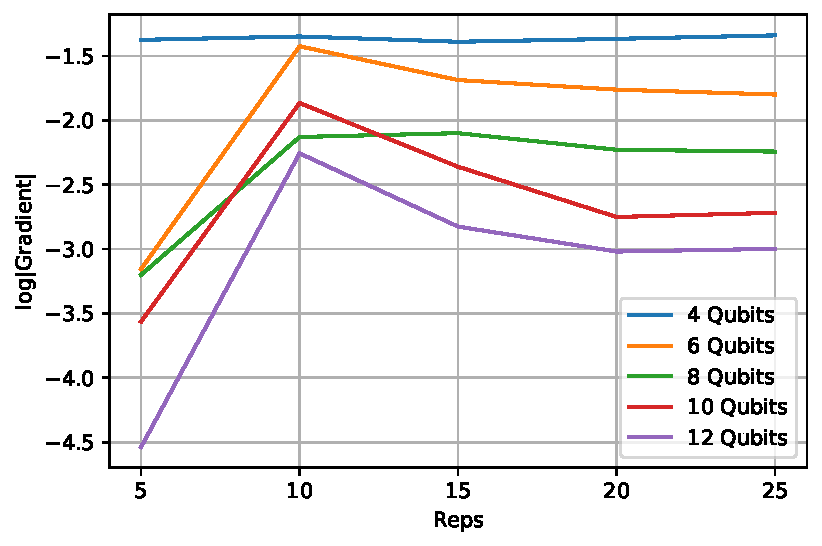
\includegraphics[width=12cm]{latex/figures/vanishing_gradient_QNN.pdf}
    \caption{Average magnitude of gradients for QNNs with different ansatz repetitions and number of qubits. The QNNs utilize qubit encoding with $R_y$ rotations, the simple ansatz for processing, and parity sampling to derive an output. The QNNs are fed $N=100$ points of uniformly sampled points, where the number of features is set equal the number of qubits. }
    \label{fig:QNN_vanishing}
\end{figure}

From the above figure, we see that our implementation of QNNs results in a gradient that vanishes in the exponential regime with respect to the number of qubits. Also, the vanishing is worse for a higher number of of repetitions of the ansatz (with the exception of going from one to two repetitions, for which the gradient actually increased.) This behaviour can be explained by the fact that QNNs are a special case of PQCs. By encoding random inputs and randomly initializing the parameters, the QNN approaches essentially a random circuit as they grow deeper. As shown by \citet{McClean_2018}, and discussed in \autoref{sec:BarrenPlateus}, randomly initialized PQCs tend to produce gradients closely centered around zero as the number of qubits are increased, which we see also applies for our implementation of QNNs. (Discuss small gradient of shallow QNNs).    

%================================================================
\subsection{Vanishing Local Gradient in QCNs}\label{sec:Vanishing Local Gradients in QCNs}
%================================================================

An interesting feature of QCNs is their ability to scale up by introducing more circuits, rather than wider and deeper ones. As the gradient of QNNs tend to vanish for a high number of qubits, we want to investigate how the gradients of smaller QNNs behave when they enter as nodes in a QCN architecture. 

The QNNs used to contruct QCNs here are set up and initialized in the same manner as in \autoref{sec:Vanishing Gradient for QNNs}, but with always two repetitions of the simple ansatz(skrive om?). Also, we sample input data in the same manner, i.e. uniformly as $\mathcal{X} \sim U(-\frac{\pi}{2}, \frac{\pi}{2})^{[N,p]}$, with $N=100$ and the number of features $p$ set to the number of qubits used in the QNNs. In this section, all QCNs have 8 hidden layers and each hidden layer will utilize $d$ number of nodes. The number of qubits in each node will also be set to $d$, which will range from $4$ to $8$. Further, the outputs of each hidden layer is scaled to the interval $[-\pi, \pi]$ to make full use of the qubit encoding in the subsequent layer, as explained in \autoref{sec:Configuring QCNs and DNNs}.

In order to investigate the average behaviour of the local gradients \autoref{eq:localGradients} for each layer, we calculate their magnitude averaged over each layer, the samples and $T = 10$ different realizations. This quantity is given by \autoref{eq:magnitude local}, and is plotted in \autoref{fig:QCN_local_vanishing} for various layers of different QCNs. In addition, the standard deviation of this quantity is estimated over the different realizations, yielding a confidence interval as seen in the figure. 

\begin{figure}[H]
    \centering
    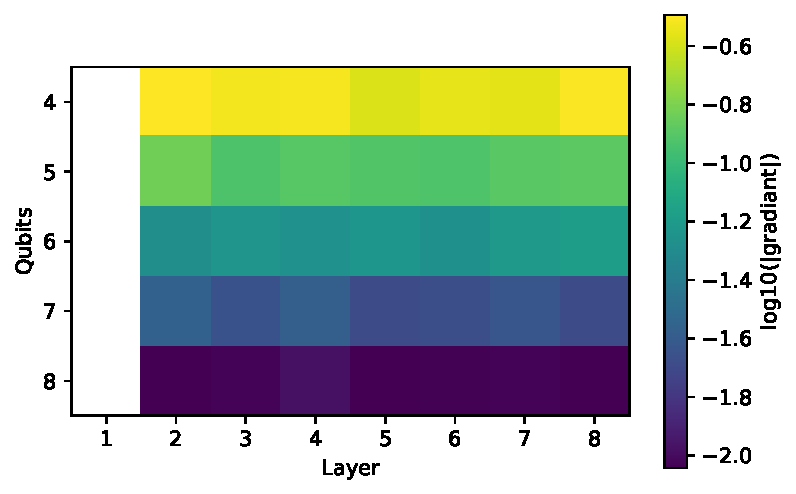
\includegraphics[width=12cm]{latex/figures/vanishing_gradient_partial_input.pdf}
    \caption{Average magnitude of local gradients \autoref{eq:localGradients} calculated for each layer for various 8 layer QCNs. This quantity was calculated using \autoref{eq:magnitude local}. The number of qubits per node are constant for each QCN, and the number of nodes per layer is set equal the number of qubits. The QNNs are fed $N=100$ points of uniformly sampled samples, where the number of features is set equal the number of qubits. The standard deviation is calculated over 10 different realizations of the model parameters.}
    \label{fig:QCN_local_vanishing}
\end{figure}

In the above figure we see the average magnitude of the local gradients for different layers and number of qubits. The local gradients of the QNNs entering the QCN model tend to vanish exponentially in the number of qubits, as with the single-circuit QNNs seen in \autoref{fig:QNN_vanishing}. However, the relative position of the QNNs along the depth of the QCN does not seem to affect the magnitude. This can be seen from the overlapping confidence intervals of the magnitudes for each number of qubits. Any variation of the average magnitude between the layers is thus likely just noise induced by the low number of $10$ parameter realizations, and does not indicate significant differences.

%================================================================
\subsection{Vanishing Total Gradient in QCNs}\label{sec:Vanishing Total Gradients in QCNs}
%================================================================

%In the previous section, it was shown that scaling up QCNs by adding more layers did not effect the number of shots needed to sufficiently estimate the local gradients of each QNN. This is in opposition to single-QNN models, whose gradient vanishes as both the number of qubits and repetitions are increase, as seen in \autoref{fig:QNN_vanishing}.

In the previous subsection, it was shown that the magnitude of local gradients of any layer were independent of the relative position of that layer in the QCN model. However, the parameters of are not updated using the local gradients directly. rather, they are updated using the total gradient \autoref{eq:derivweightsQCN}, which is calculated by combining the local gradients using back propagation \autoref{eq:errorQCN}. We need to investigate how the magnitude of the total gradient \autoref{eq:derivweightsQCN} behaves as a function of layers and qubits. 

In this section, the total gradient is calculated using the local gradients from the same numerical experiment as in \autoref{sec:Vanishing Local Gradients in QCNs}. As previously, the magnitude of the total gradient is averaged over each layer, the samples and 10 realisations of the parameters using \autoref{eq:magnitude QCN DNN}. This quantity is plotted in \autoref{fig:QNC_vanishing_total} for different layers and number of qubits. For comparison, it also shows the magnitude of the total gradient of a DNN with the same number of layers and similar number of parameters as the biggest QCN.

\begin{figure}[H]
    \centering
    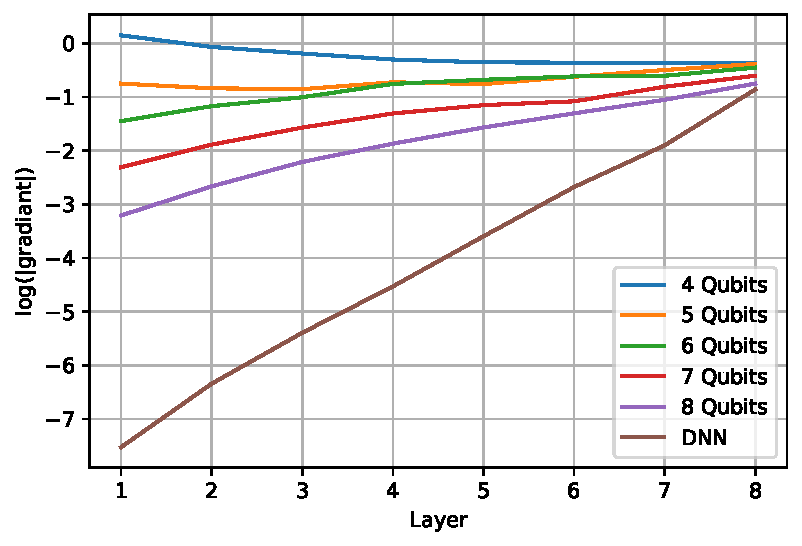
\includegraphics[width=12cm]{latex/figures/vanishing_gradient_total.pdf}
    \caption{Average magnitude of the total gradient \autoref{eq:derivweightsQCN} calculated for each layer for various 8 layer QCNs. This quantity is calculated using \autoref{eq:magnitude QCN DNN}. The number of qubits per node are constant for each QCN, and the number of nodes per layer is set equal the number of qubits.  For comparison, the same quantity is also calculated for an 8 layer DNN.(more info about DNN)} 
    \label{fig:QNC_vanishing_total}
\end{figure}

From \autoref{fig:QNC_vanishing_total}, we see that the total gradient for a given layer in the DNN tends to vanish exponentially in the number of layers after it. This is a well-known phenomenon for classical neural networks, often explained by the saturation of the activation function during feed forward\cite{shalevshwartz2017failures}. (Write about this under neural network theory).

As with the DNN, also the QCNs exhibits vanishing total gradient with increasing number of layers, with a strong dependence on the number of qubits in each node. Seen in \autoref{fig:QCN_local_vanishing}, the total gradient vanishes faster for higher number of qubits in each node. This phenomenon can be related to the magnitude of the local gradients. As the error \autoref{eq:lastLayerErrorQCN} of the QCN is propagated backwards using \autoref{eq:errorQCN}, it accumulates the local gradients $\frac{\partial \boldsymbol{a}^{l+1}_k}{\partial \boldsymbol{a}^{l}_j}$ as factors. In the case that these factors are large, the error will tend to decrease slowly, and hence also the total gradient. This is the case for architectures with few qubits per node, as discussed in \autoref{sec:Vanishing Local Gradients in QCNs}. However, as the number of qubits increase, the local gradients will tend to decrease. Accumulating small factors will cause the error to decrease faster, exponentially so for each layer. In a sense, this vanishing of local gradients with increasing number of qubits is analogous to the saturation of the activations for classical networks.

%================================================================
\subsection{Discussion}\label{sec:Vanishing Gradient Phenomenon Discussion}
%================================================================
The results of \autoref{sec:Vanishing Gradient for QNNs} show that up-scaling of QNNs by increasing the number of qubits and repetitions of the ansatz results in an exponential decay of their gradients. As explained in \autoref{sec:BarrenPlateus}, this means that exponentially many shots are required in order to obtain a good signal-to-noise when estimating the gradient. If the gradient is too noisy, optimization using gradient descent and similar methods may result in essentially a random walk in parameter space that fail to converge (kilde). This becomes even more problematic in the presence of addition noise introduced by noisy hardware, as discussed in \autoref{sec:Noisy Simulation}. Ultimately, this indicate that the training of QNNs can become intractable as they are up-scaled to solve harder learning problems.    

In \autoref{sec:Vanishing Local Gradients in QCNs}, we see that the local gradients of QCNs also vanish exponentially in the number of qubits, but are independent of the overall number of layers of the QCN. In other words, the local gradients of any layer are unaffected by outputs produced by the previous layer. This suggests that QCNs can be up-scaled by making them deeper, without affecting the magnitude of the local gradients. Consequently, a constant number of shots can be used for each node during estimation to obtain a certain signal-to-noise ratio, making their estimation tractable on a quantum computer. 

Even though the magnitude of local gradients of QCNs tends to stay constant in the number of layers, we see in \autoref{sec:Vanishing Total Gradients in QCNs} that back propagation still induce an exponentially vanishing total gradient for sufficiently many qubits. This is due to the accumulation of small factors when the local gradients are combined using back propogation. This behaviour is similar to that of DNNs, with the gradient vanishing faster for initial layers. However, the vanishing was not as severe for a conservative number of qubits. For 4 qubits, the gradient actually tended to increase. For 8 qubits, and presumably above, the gradient vanished faster for QCNs than for similarly sized DNN.  

An interesting observation is that the vanishment caused by back propagation happens in a purely classical part of the optimization, with the local gradients stored as floating-point numbers. This means that even though the total gradient tends to decrease exponentially with the number of layers, it does not introduce an exponential overhead on the quantum computer by requiring more shots. This is true, however, for single-QNN models as discussed in \autoref{sec:BarrenPlateus}. Put another way, QCNs' use of several smaller circuits, rather than one big, moves the estimation of vanishing quantities (the gradient) from quantum expectation values to classical computation. 



%================================================================
\section{Investigating the Loss Landscape}\label{sec:Investigating the Loss Landscape}
%================================================================
We explore the geometry of the loss landscape of various models and quantify its degree of distortion and flatness by studying the eigenvalue spectrum of the EFIM \autoref{eq:EmpiricalFisher}. Looking at \autoref{eq:EmpiricalFisher}, we see that the EFIM, unlike the Hessian, is independent of targets $y^{(i)}$. This makes the analysis data agnostic, and serves to characterise the architectures themselves. The input data $\mathcal{X} = \{\boldsymbol{x}^{(1)}, \cdots, \boldsymbol{x}^{(N)}\}$ used for calculating the EFIM is sampled randomly from a standard normal distribution as $\mathcal{X} \sim N(0,1)^{[N,p]}$. This ensures that the input is evenly sampled from feature space and is consistent with the analysis of \citet{abbas2020power}. Here, we use $N=200$ samples and either $p=4$ or $p=6$ inputs, depending on the model. For each model, the EFIM is calculated 10 times for different random initializations of the parameters. The resulting spectrum is then averaged over the 10 initializations to produce more a significant results. For a complete description of the models analysed in this section, see \autoref{tab:FIM models}.

\begin{table}[H]
\caption{Description of the architecture of the models analysed in this section. The QNN and QCN models use exact evaluation of parity to derive outputs (see \autoref{sec:Exact Expectation Value} and \autoref{sec:Inference}). The DNN models uses tanh activation in all layers. The parameters of the models are appropriately initialized as presented in \autoref{sec:Initialization}.} 
\centering
\begin{tabular}{|l|l|l|l|l|l|l|l|}
\hline
Model &Type & Qubits& Reps & Layers & Width & Encoder        & $n_{\theta}$ \\ \hline
A    & QNN & 4& 18   & 1      & 4     & RZZ Encoding   & 72  \\ \hline
B    & QCN & 4& 3    & 2      & 4     & Qubit Encoding & 60 \\ \hline
C    & QCN & 4& 2    & 3      & 4     & Qubit Encoding & 72  \\ \hline
D    & QCN & 4& 1    & 5      & 4     & Qubit Encoding & 68  \\ \hline
E    & DNN & NA& NA   & 3      & 6     & NA             & 79 \\ \hline
F    & QNN & 6& 26   & 1      & 6     & RZZ Encoding   & 156  \\ \hline
G    & QCN & 6& 4    & 2      & 6     & Qubit Encoding & 168 \\ \hline
H    & QCN & 6& 2    & 3      & 6     & Qubit Encoding & 156  \\ \hline
I    & QCN & 6& 1    & 5      & 6     & Qubit Encoding & 150  \\ \hline
J    & DNN & NA& NA   & 3      & 9     & NA             & 163 \\ \hline
\end{tabular}
\label{tab:FIM models}
\end{table}

\autoref{fig:FIM Comparison} compares the EFIM spectrum of QNNs, QCNs and DNNs. Their architectures are chosen so that the models have approximately equal number of parameters. This is to ensure a fair comparison. 

\begin{figure}[H]
    \centering
    \begin{subfigure}[t]{0.5\textwidth}
        \centering
        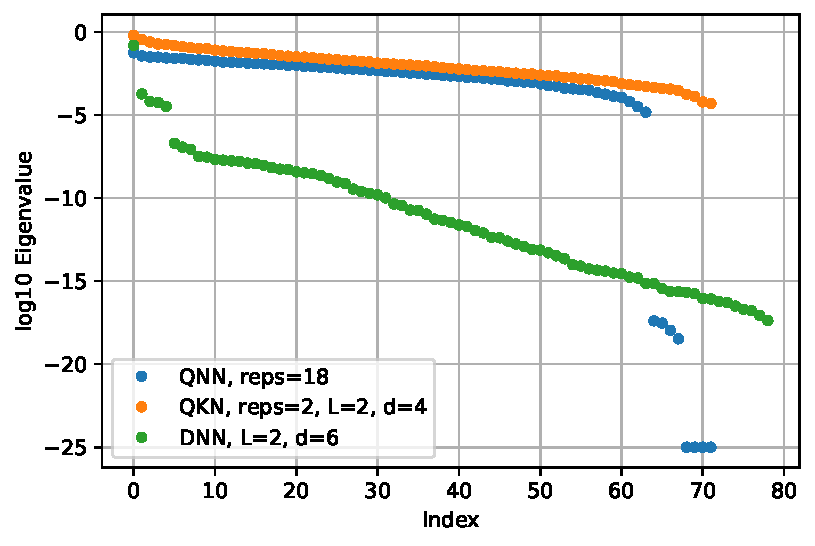
\includegraphics[height=1.9in]{latex/figures/FIM_qubits_4.pdf}
        \caption{Lorem ipsum}
        
    \end{subfigure}%
    ~ 
    \begin{subfigure}[t]{0.5\textwidth}
        \centering
        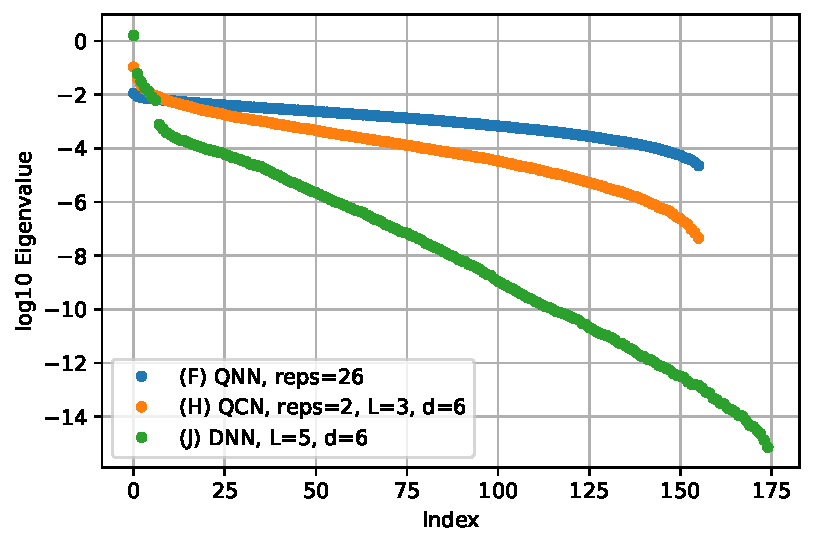
\includegraphics[height=1.9in]{latex/figures/FIM_qubits_6.pdf}
        \caption{Lorem ipsum}
    \end{subfigure}
    \caption{Comparison of EFIM eigenvalue spectrum between QNNs, QCNs and DNNs. For details about the architectures, see \autoref{tab:FIM models}. The EFIM is calculated using $N=200$ points of uniformly sampled points, where the number of features are set equal the number of qubits. The EFIM spectrum is finally averaged over 10 different model realizations.}
    \label{fig:FIM Comparison}
\end{figure}

Looking at the spectra of the DNNs in \autoref{fig:FIM Comparison}, we see the characteristic result of a singular large eigenvalue, with the rest sitting close to zero. This indicates that DNN models exhibit a loss landscape that is very flat in all but one direction, where it is extremely distorted. We also see that the spectra of the our implementation of QNNs are much more uniformly distributed compared to the DNN models. This results in a loss landscape that is significantly distorted in most directions, rather than just one. 

Moving over to the QCNs, we see from \autoref{fig:FIM Comparison} that the spectra of the three layer QCNs exhibit much the same uniformity as the QNNs. A more thorough comparison between different QCNs can be seen in \autoref{fig:FIM QCN}. In this figure, we vary the number of layers of the QNCs and the number of repetitions (i.e. the number of times the ansatz is repeated for each node), while keeping the total number of parameters roughly constant. In doing this, we get to precisely shift how much of the complexity of a given QCN results from the complexity of each node or the overall structure of the network.

\begin{figure}[H]
    \centering
    \begin{subfigure}[t]{0.45\textwidth}
        \centering
        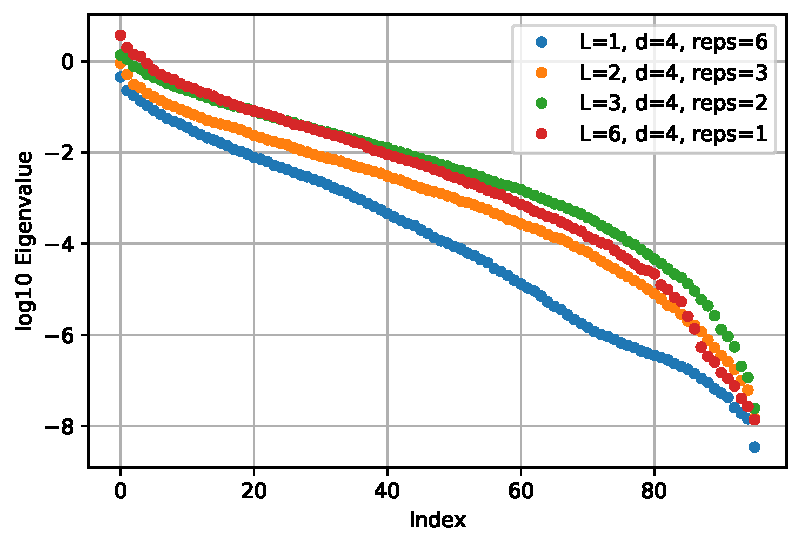
\includegraphics[height=1.8in]{latex/figures/FIM_qubits_4_comparison.pdf}
        \caption{Comparison of the EFIM eigenvalue spectrum for different 4-qubit QNNs and QCNs.}
        \label{fig:FIM QCN a}
    \end{subfigure}%
    ~ 
    \begin{subfigure}[t]{0.45\textwidth}
        \centering
        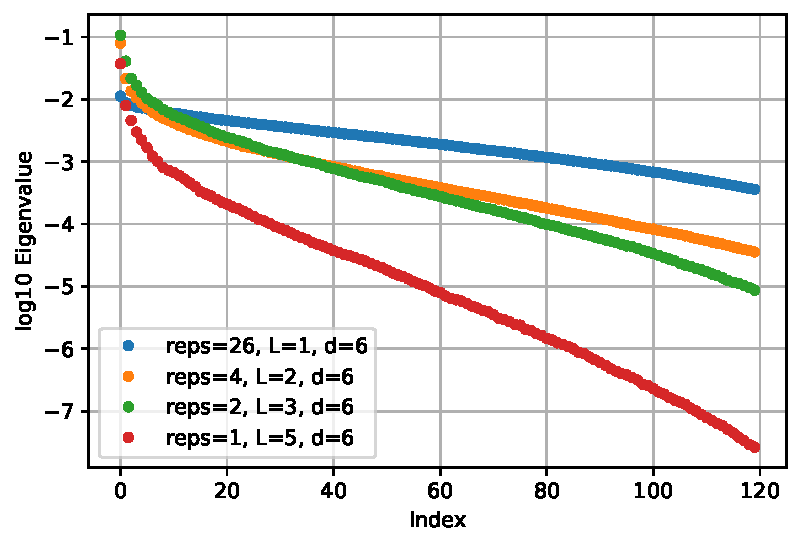
\includegraphics[height=1.8in]{latex/figures/FIM_qubits_6_comparison.pdf}
        \caption{Comparison of the EFIM eigenvalue spectrum for different 6-qubit QNNs and QCNs.}
        \label{fig:FIM QCN b}
    \end{subfigure}
    \caption{Comparison of the EFIM eigenvalue spectrum between different QNNs and QCNs. For details about the architectures, see \autoref{tab:FIM models}. The EFIM is calculated using $N=200$ points of uniformly sampled points, where the number of features is set equal the number of qubits for each model. The EFIM spectrum is finally averaged over 10 different model realizations to produce a more significant result.}
    \label{fig:FIM QCN}
\end{figure}

\autoref{fig:FIM QCN a} shows that, for four qubits, the spectra of the different QCNs exhibit roughly the same uniformity as the QNN, with the eigenvalues staying within roughly an order of magnitude of each-other. Going up to six qubits, \autoref{fig:FIM QCN b} shows that the spectrum tends to concentrate more around zero for increasing number of layers. This is likely related to the vanishing of the gradient induced by back propagation. For four qubits, this is not as big of a problem since the local gradients are relatively big and hence also the total gradient. However, for six qubits, the local gradients tend to vanish. This results in the gradient vanishing faster when increasing the number of layers, which in turn results in a flatter landscape. 


%================================================================
\subsection{Discussion}\label{sec:Loss Landscape Discussion}
%================================================================
The highly uneven EFIM spectrum of DNNs indicates a loss landscape that is strongly distorted in one direction and mostly flat otherwise. This result is consistent with the findings of \citet{karakida2019universal} and \citet{abbas2020power}. The former authors point out that strong distortions in some directions indicate that the model outputs are very sensitive to changes in parameter space in exactly these directions, and likewise not sensitive to changes in the others. This tend to slow training when using gradient descent and similar methods, as too high learning rate leads to overstepping in the distorted directions, while a low learning rate changes the model insignificantly in the flat directions. 

For the QNNs, we found the EFIM spectrum to be much more uniform than that of a comparable DNN. \citet{abbas2020power} came to the same conclusion for their QNN models, and argued that this uniformity of the spectrum meant that landscape was more well-condition for optimization, and thus should train faster. They strengthened this hypothesis by showing experimentally that QNNs reduced error faster than DNNs for equal number of training iterations. 

We found that QCNs with four qubits exhibit similar uniformity of the EFIM spectrum as QNNs. For six qubits, the spectrum became increasingly more skewed, with a worsening effect for more layers. However, they still showed several order of magnitude larger eigenvalues that DNNs, suggesting that small-scale QCNs should train comparably faster than DNNs, like QNNs.

%================================================================
\section{Expressivity}\label{sec:Expressivity}
%================================================================
We will investigate the expressivity of QCNs and DNNs using the trajectory length method of \citet{raghu2017expressive}, as described in \autoref{sec:TrajectoryLength}. The trajectory length will be first studied for randomly initialized QCNs for varying number of qubits in each node. Then, for some selected QCNs, the trajectory length will be investigated as the models are gradually fitted on 2D mixed Gaussian data. The results in both cases will be compared to similar DNNs, with approximately the same number of parameters for fair comparison. We will use a input trajectory  used will be circle $\boldsymbol{x}(t_i) \in \mathbb{R}^2$ with radius $\frac{\pi}{2}$ and centered around $0$, divided up into $1000$ equally spaced point. The input trajectory and 2D mixed Gaussian data will be pre-processed appropriately, depending on the model, as described in \autoref{sec:Pre-processing Input}.

%================================================================
\subsection{Untrained Models}\label{sec:Untrained Models}
%================================================================

In this subsection, we investigate the same QCN and DNN architectures as formulated in \autoref{sec:Vanishing Local Gradients in QCNs}, initialized randomly in the same manner. \autoref{fig:TL_untrained} shows how the trajectory length varies as a function of layer, when the different models are fed the circle trajectory $\boldsymbol{x}(t_i)$ defined earlier.

%All layers have $d$ number of nodes, and all nodes have $d$ number of qubits. $d$ ranges from $4$ to $8$. For comparison, the trajectory length is also calculated for an 8-layer DNN with approximately the same number of parameters as the biggest QCN. The QCNs and the DNN are randomly initialized as in \autoref{sec:Vanishing Gradient Phenomenon}.

\begin{figure}[H]
    \centering
    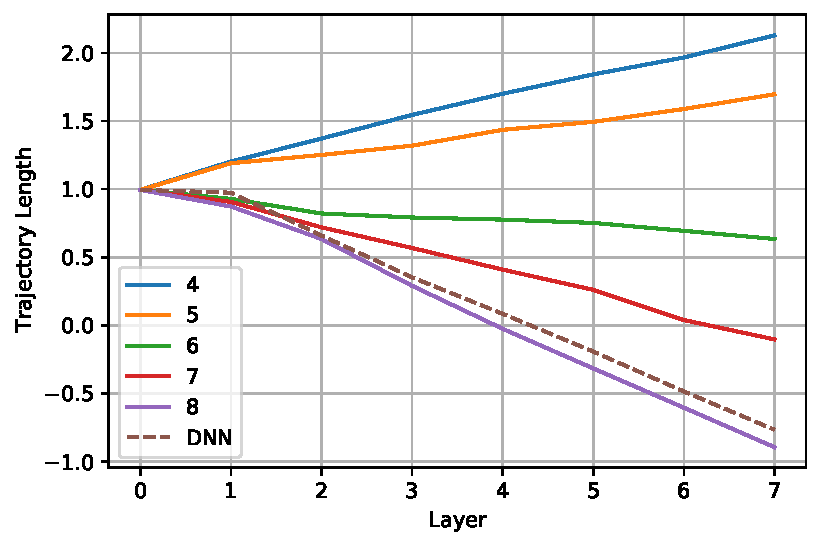
\includegraphics[width=12cm]{latex/figures/TL_untrained.pdf}
    \caption{}
    \label{fig:TL_untrained}
\end{figure}

\autoref{fig:TL_untrained_projection}, accompanying \autoref{fig:TL_untrained}, shows the trajectories of selected models and layers, projected onto 2D. The rows correspond to the 4 qubit QCN, 8 qubit QCN and DNN, from top to bottom. The columns correspond to the first layer, second layer, third layer and last layer, left to right.   

\begin{figure}[H]
    \centering
    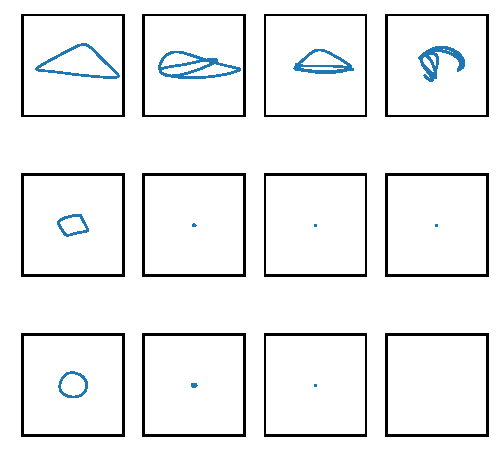
\includegraphics[width=12cm]{latex/figures/TL_untrained_projection.pdf}
    \caption{}
    \label{fig:TL_untrained_projection}
\end{figure}

%In \autoref{fig:TL_untrained}, we see that the untrained DNN exhibits an exponential decrease in trajectory length as it is being transformed by each layer. From \autoref{fig:TL_untrained_projection}, we see this manifesting itself as the trajectory concentrating around some mean, progressively more for each layer. This shows that randomly initialized DNNs can tend to compute functions which are not very sensitive to the input, which was shown experimentally by \citet{raghu2017expressive} to be possible in practical settings. 

From \autoref{fig:TL_untrained}, we see that the trajectory length of QCNs with 4 and 5 qubits tend to grow exponentially with the number of layers. This growth is however diminishing as the number of qubits increase, and switches over to an exponential decay for 6 qubits and above. For 8 qubits, the decay is similar to that of the DNN with similarly many parameters. Comparing the results to \autoref{fig:TL_untrained_projection}, we see how the increasing and decreasing trajectory length manifests themselves. Seen from the top row, the trajectory produced by the 4 qubit QCN tends to become increasingly distorted and complex. This is similar to the behaviour of classical networks seen in \autoref{fig:trajectoryLengthExample}, produced by \citet{raghu2017expressive}, and shows that also QCNs can compute functions exponentially complex in the number of layers. In contrast, the trajectory of the 8 qubit QCN and DNN (seen in the next two rows) can be seen to gradually concentrate for each layer, resulting in a function that is very little sensitive to the input.  


%================================================================
\subsection{Trained Models}\label{sec:Trained Models}
%================================================================
\citet{raghu2017expressive} showed that networks that initially don't lie in the exponential growth regime can be pushed there via training. In this subsection, we will train different models by incrementally fitting them to the 2D mixed Gaussian data. The trajectory length will be recalculated for each layer after each increment. The models being investigated here are two four layer QCNs with 6 and 7 qubits, respectively, with each node having the same architecture as in \autoref{sec:Untrained Models}. These will be compared with DNNs with approximately same number of parameters. For more information about the models, see \autoref{tab:TL models}. All the models are trained using Adam optimizer with the standard hyperparameters and a learning rate of $0.1$. The QCNs are trained for a total of $20$ epochs in increments of $5$. In order to produce a fair comparison, the DNNs will not be trained for the same increments of epochs. Rather, they will be trained until they achieve approximately the same MSE on the training set as the QCNs, for each increment. In this way, we get to compare the expressivity of QCNs and DNNs that fit the data to an equal degree. \autoref{fig:TL_trained} shows how the trajectory length changes as the different models presented here are incrementally trained, for each layer. 

\begin{figure}[H]
    \centering
    \begin{subfigure}[t]{0.5\textwidth}
        \centering
        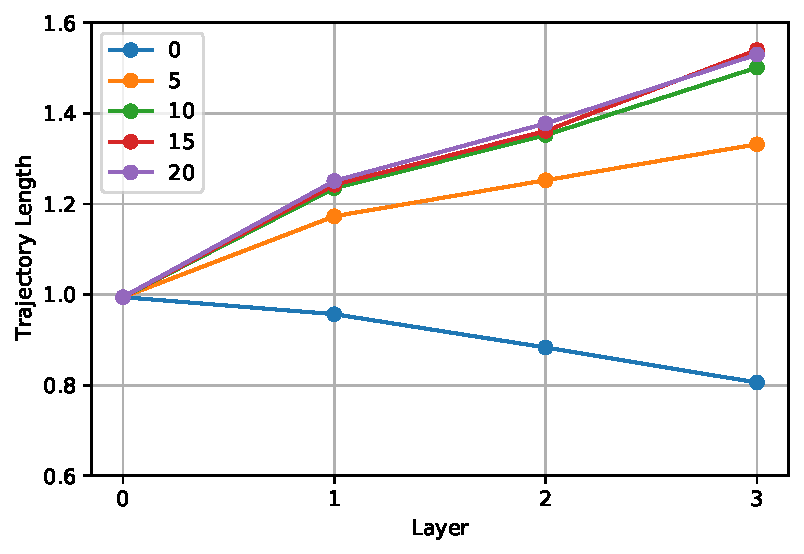
\includegraphics[height=1.9in]{latex/figures/TL_trained_QCN_qubit_6.pdf}
        \caption{QCN, 6 qubits. 228 parameters.}
        \label{fig:TL_trained_A}
        
    \end{subfigure}%
    \hfill 
    \begin{subfigure}[t]{0.5\textwidth}
        \centering
        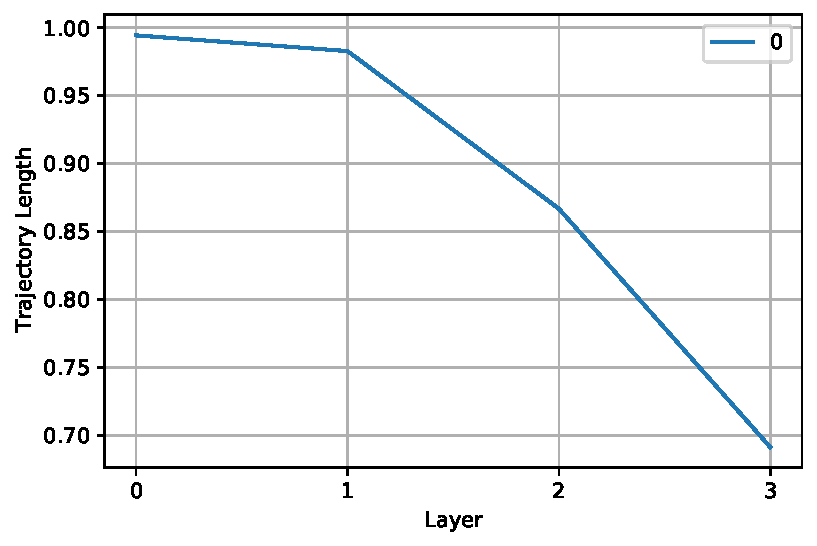
\includegraphics[height=1.9in]{latex/figures/TL_trained_QCN_qubit_7.pdf}
        \caption{QCN, 7 qubits. 308 parameters.}
        \label{fig:TL_trained_B}
    \end{subfigure}
    \vskip\baselineskip
    \begin{subfigure}[t]{0.5\textwidth}
        \centering
        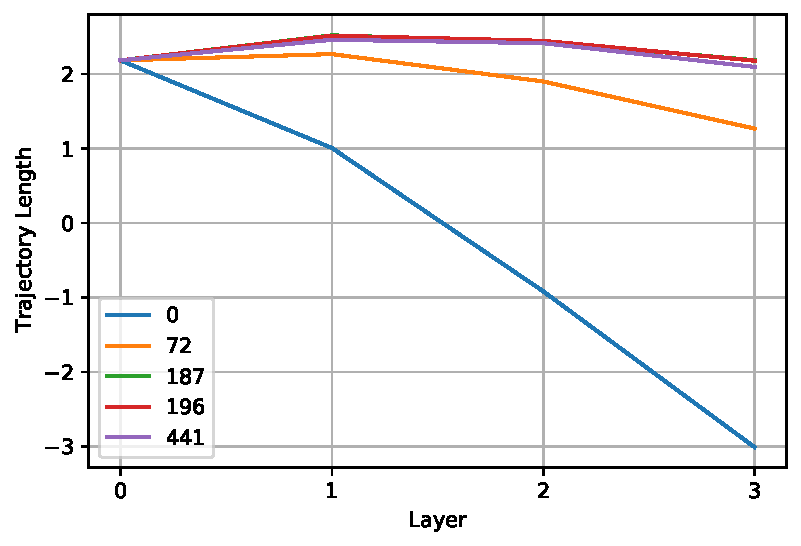
\includegraphics[height=1.9in]{latex/figures/TL_trained_DNN_nodes_9.pdf}
        \caption{DNN, 9 nodes. 217 parameters.}
        \label{fig:TL_trained_C}
        
    \end{subfigure}%
    \hfill 
    \begin{subfigure}[t]{0.5\textwidth}
        \centering
        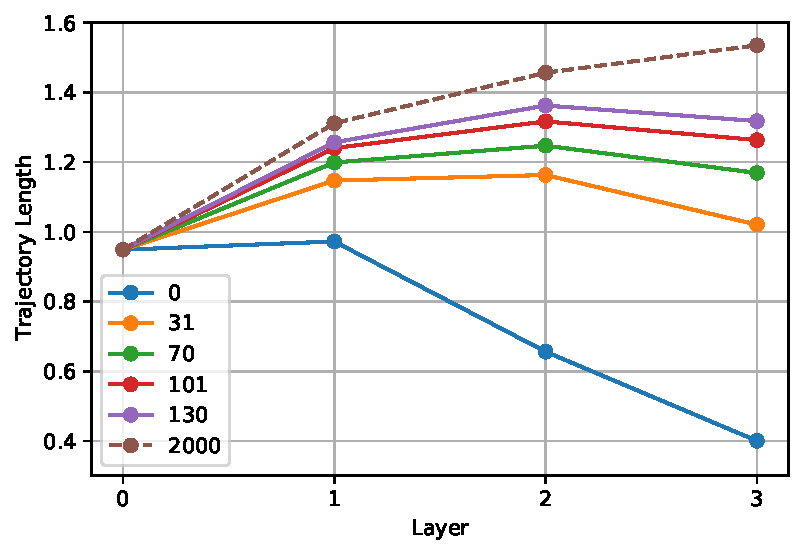
\includegraphics[height=1.9in]{latex/figures/TL_trained_DNN_nodes_11}
        \caption{DNN, 11 nodes. 309 parameters.}
        \label{fig:TL_trained_D}
    \end{subfigure}
    \caption{Caption place holder}
    \label{fig:TL_trained}
\end{figure}

From \autoref{fig:TL_trained}, we see that training the QCNs and DNNs progressively increases the trajectory length of the models. After only $5$ epochs, the trajectory length of the 6 qubit QNC enters the exponential growth regime. This demonstrates that randomly initialized QCNs can be made to produce complex functions through training, even though their outputs initially tend to concentrate around a mean, as shown in \autoref{fig:TL_untrained}. The 7-qubit QCN is brought into the exponential growth regime after $10$ epochs, twice the amount required for 6 qubits. 

Moving over to the corresponding DNNs, we see that they fail to enter the same exponential growth regime as the QCNs, even when trained until they fit the data to the same degree. This indicates that QCNs, in this context, may be more expressive than DNNs for the same number of parameters.  

\begin{table}[H]
\centering
\begin{tabular}{|l|l|l|l|l|l|}
\hline
Model &Type & Qubits& Layers & Nodes &$n_{\theta}$ \\ \hline
A    & QCN & 6 &  4 & 6& 228   \\ \hline
B    & QCN & 7 &  4 & 7& 308 \\ \hline
C    & DNN & NA&  4 & 9& 217  \\ \hline
D    & DNN & NA&  4 & 11& 309  \\ \hline
\end{tabular}
\caption{Stuff.} 
\label{tab:TL models}
\end{table}


%================================================================
\subsection{Single Node Expressivity}\label{sec:Single Node Expressivity}
%================================================================
To attempt elucidating the discrepancy of expressivity between QCNs and DNNs, we investigate the functional form of node outputs for QCNs and DNNs. To do this, we utilize two 4-qubit QNN with qubit encoding and two repetitions of the simple ansatz. We encode data in two different ways: With the first QNN, we will encode a single feature $x$ to its first. With the second QNN, we pad the samples by repeating the feature  such as $\boldsymbol{x} = (x, x, x, x)$ and encode it in the usual way, creating a tensorial feature map for $x$ as explained in \autoref{sec:Tensorial Feature Mapping}. For comparison, we also feed the padded samples $\boldsymbol{x}$ to a single DNN node with Tanh activation. In \autoref{fig:activations}, we plot the output the different nodes for different parameters realizations and values of $x$.

\begin{figure}[H]
    \centering
    \begin{subfigure}[t]{0.5\textwidth}
        \centering
        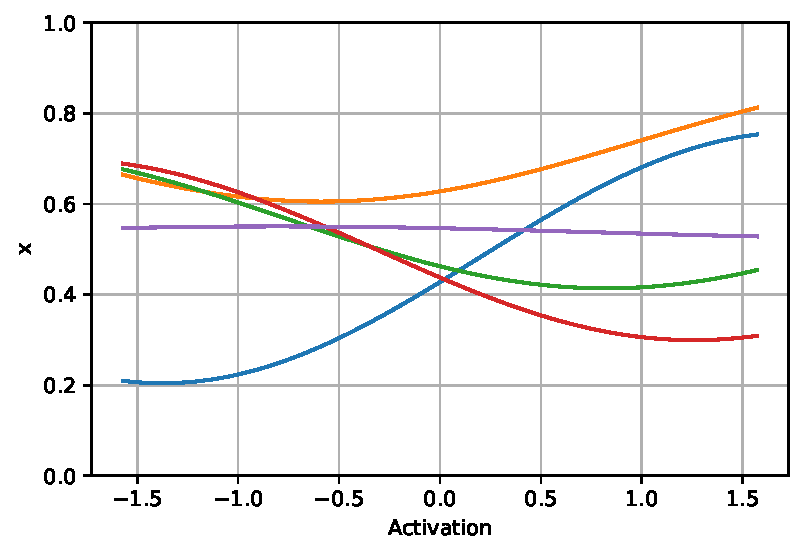
\includegraphics[height=1.9in]{latex/figures/activation_qnn_1.pdf}
        \caption{Lorem ipsum}
        \label{fig:activations single}
        
    \end{subfigure}%
    \hfill 
    \begin{subfigure}[t]{0.5\textwidth}
        \centering
        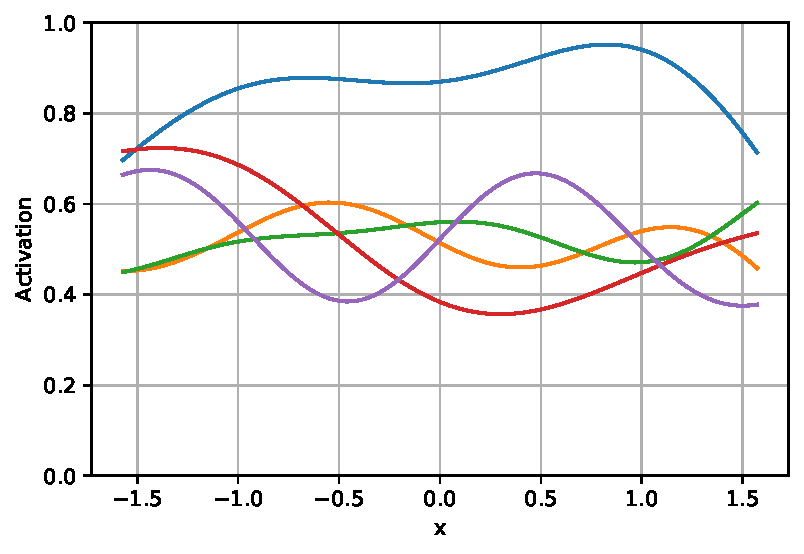
\includegraphics[height=1.9in]{latex/figures/activation_qnn_4.pdf}
        \caption{Lorem ipsum}
        \label{fig:activations tensorial}
    \end{subfigure}
    \vskip\baselineskip
    \begin{subfigure}[t]{0.5\textwidth}
        \centering
        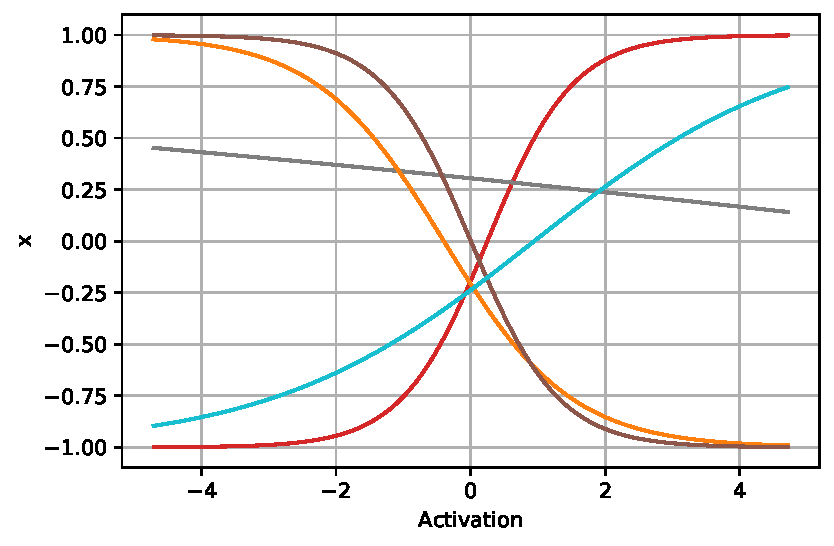
\includegraphics[height=1.9in]{latex/figures/activation_dnn.pdf}
        \caption{Lorem ipsum}
        \label{fig:activations DNN}
    \end{subfigure}%
    \caption{Caption place holder}
    \label{fig:activations}
\end{figure}

In \autoref{fig:activations single}, we see the output of the QNN encoding a single feature. Since the samples are only encoded once, it doesn't compute a state whose amplitudes represent polynomials of the input. Consequently, the outputs resemble simple trigonometric functions. Seen from \autoref{fig:activations tensorial}, utilizing the tensorial feature mapping enables the QNN to produces a much flexible output, reflecting the polynomial representation of the data in the prepared state. \autoref{fig:activations DNN} shows that the output of the DNN node is constrained to the functional form of the tanh activation function.   




%================================================================
\subsection{Discussion}\label{sec:Discussion Expressivity}
%================================================================

For higher number of qubits, we saw from \autoref{fig:TL_untrained_projection} that the trajectory of untrained QNCs tend to concentrate progressively for each layer they pass through. This is a manifestation of the phenomenon where PQC outputs tends to concentrate around their average value when the number of qubits is increased. Since each node is a QNN, which is a type of PQC, QCN are also subject to this. As the inputs are sequentially transformed by each layer in the QCN, this concentration of the outputs is in fact applied multiple times, causing an exponential decrease of the trajectory length, as seen in \autoref{fig:TL_untrained}.

From \autoref{fig:TL_trained} we see that training brought the QCNs into the exponential growth regime, increasing the sensitivity of the node outputs with respect to the inputs. In other words, optimizing the QCNs updates the parameters in a way that brings structure to each of the circuits, moving them away from being random circuits. This causes the outputs to no longer concentrate around the mean, which in turn lets the model compute more complex functions. 

Comparing \autoref{fig:TL_trained_A} and \autoref{fig:TL_trained_B}, we see that the 7-qubit QCN required twice the number of epochs to enter the exponential growth regime compared to the 6-qubit QCN. As discussed in \autoref{sec:Vanishing Gradient Phenomenon}, increasing the number of qubits makes the magnitude of the gradient exponentially smaller. Thus, a larger number of epochs, potentially exponentially so, are required to significantly change the parameters such that the nodes no longer resemble random circuits. This might produce a significant overhead for QCNs with a high number of qubits, making them very slow to train to be expressive.  

Looking at \autoref{fig:TL_trained_C} and \autoref{fig:TL_trained_D}, we see that the corresponding DNNs fail to enter the exponential growth regime, even after training the models for a number of epochs that result in the same MSE as the QCNs. The DNNs approached exponential growth first after more than an order magnitude more epochs. This suggests that QCNs can be trained to be more expressive than DNNs of similar number of parameters. How can we explain this increased expressivity? As discussed in \autoref{sec:Single Node Expressivity}, qubit encoding several features results in a representation of exponentially many interactions in the data, which also results in a more flexible output. The different parameter realizations produce very different functional outputs, enabling the QCN to learn unique activations for each node. This is contrast to the outputs of the DNNs, which is very constrained by the Tanh activation function. 

%A possible explanation for this is that the mathematical transformation applied by the QCN is in a way more powerful compared to DNNs. Typically, sufficiently deep PQCs are conjectured to be intractable for classical computers to simulate efficiently \cite{abbas2020power}\cite{lloyd2018quantum}. Stated in \autoref{sec:Multiple Qubits}, as the numbers of qubits $n$ increase, the dimensionality of the resulting Hilbert space grows exponentially as $d = 2^n$. It follows that gates applied on this space is mathematically represented as a $d\times d$ matrices, which causes an exponential overhead on classical computers. In this sense, the encoding and unitary transformations of each QCN node constitutes a harder computation than the affine transformation and non-linearity of DNN nodes. Still, even though a computation is harder, it does necessarily result in the computation of a richer, more complicated function. For example, it was shown from \autoref{fig:TL_untrained} that the opposite is true for randomly initialized QCNs. However, the increasing trajectory length seen in \autoref{fig:TL_trained} suggest that(elaborate). 

%================================================================
\section{Training Models on Mixed Gaussian Data}\label{sec:Training Models}
%================================================================
In this section, we will study the ability of various models to fit one, two and three dimensions mixed Gaussian data. For more details on the data, see \autoref{sec:Mixed Gaussian Data}. We will train QNNs, QCN and DNNs with varying complexity and use MSE on the training data to evaluate how good the fit is. This will be done first in the ideal case, with exact calculation of outputs. Then, we will repeat the training using the  simulated the noise model of the Santiago quantum computer(kilde). The hyper parameters, such as number of layers, nodes and qubits, are chosen by trial and error such that the results QCNs are relatively small in number of parameters, but still fit the data sufficiently. The QNNs and DNNs are then chosen such that they have similar number of parameters as the QCNs. For a detailed description of the models trained in this section, see \autoref{tab:training models}.

\begin{table}[H]
\centering
\caption{Hyper-parameters of the different models fitted to the one, two, and three dimensional mixed Gaussian data. Here, "Qubits" refer to the number of qubits used in each circuit, and "Reps" refer to the number of repetitions of the simple anzats \autoref{eq:simple ansatz}.} 
\begin{tabular}{|l|l|l|l|l|l|l|l|}
\hline
Model& Type& Data& Qubits& Reps& Layers & Nodes &$n_{\theta}$ \\ \Xhline{3\arrayrulewidth}
A    & QNN & 1D  & 4     & 5&NA     & NA& 20   \\ \hline
B    & QCN & 1D  & 4     & 1&2      & 4& 20 \\ \hline
C    & QCN & 1D  & 4     & 2&2      & 4& 40  \\ \hline
D    & DNN & 1D  & NA    & NA&2      & 13& 40  \\ \Xhline{3\arrayrulewidth}
E    & QNN & 2D  & 4     & 10&NA     & NA& 40  \\ \hline
F    & QCN & 2D  & 4     & 1&3      & 4& 40  \\ \hline
G    & QCN & 2D  & 4     & 2&3      & 4& 80  \\ \hline
H    & DNN & 2D  & NA    & NA&3      & 7& 85  \\ \Xhline{3\arrayrulewidth}
I    & QNN & 3D  & 5     & 11&NA     & NA& 55  \\ \hline
J    & QCN & 3D  & 5     & 1&3      & 5& 55  \\ \hline
K    & QCN & 3D  & 5     & 2&3      & 5& 110  \\ \hline
L    & DNN & 3D  & NA    & NA&3      & 8& 113  \\ \hline
\end{tabular}

\label{tab:training models}
\end{table}

For the QNNs trained in this section, we will utilize RZZ encoding \autoref{fig:Rzzencoding} in an effort to increase the flexibility of the model. From \autoref{sec:RZZencoding}, we know that the circuit depth of this encoding scales as $\mathcal{O}(p^2)$, where $p$ is the number of features. To get a constant depth across the 1D, 2D and 3D Gaussian data, we will repeat features until all the data sets have the same number of features: For the 1D data, we repeat the one feature three times: $(x_1) \rightarrow (x_1, x_2, x_3)$. For the 2D data, we repeat the first feature once: $(x_1, x_2) \rightarrow (x_1, x_2, x_1)$. The 3D data is left unchanged, since it already has three features. In this way, RZZ encoding prepares similarly complicated encoding for all data sets. 


%================================================================
\subsection{Ideal Simulation}\label{sec:Ideal Simulation}
%================================================================
\autoref{fig:trained ideal} shows the MSE during training of the models defined in \autoref{tab:training models} on the one, two and three dimensional mixed Gaussian data. All models are trained for 100 epochs, using ideal simulation. In order to produce a more significant result, each model is randomly initialized 10 times and trained separately. The resulting MSE for each model is then averaged over the 10 runs and plotted with fill corresponding to one standard deviation. In this way, we get to see the average model behaviour during training and how it varies between different runs. \autoref{tab:training models mse} shows the final MSE after 100 epochs for the various models. In addition, the final MSE after $10^4$ epochs is included for the DNNs.   

\begin{figure}[H]
    \centering
    \begin{subfigure}[t]{0.45\textwidth}
        \centering
        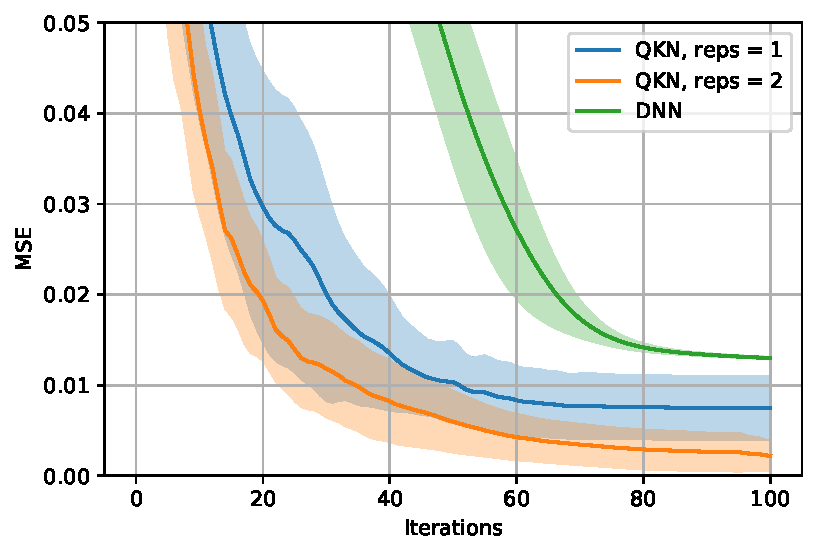
\includegraphics[height=1.9in]{latex/figures/1D_gaussian_data_fit.pdf}
        \caption{MSE of models trained on 1D mixed Gaussian data.}
        
    \end{subfigure}%
    \hfill 
    \begin{subfigure}[t]{0.45\textwidth}
        \centering
        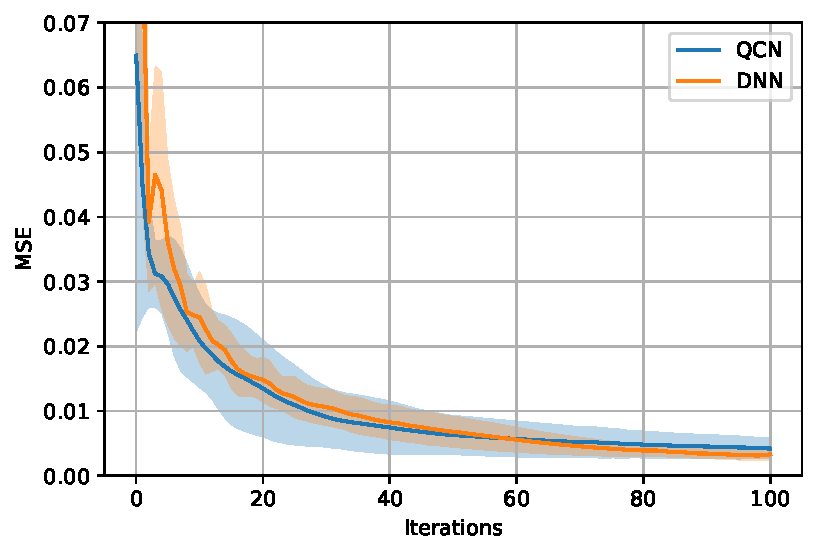
\includegraphics[height=1.9in]{latex/figures/2D_gaussian_data_fit.pdf}
        \caption{MSE of models trained on 2D mixed Gaussian data.}
    \end{subfigure}
    \vskip\baselineskip
    \begin{subfigure}[t]{0.45\textwidth}
        \centering
        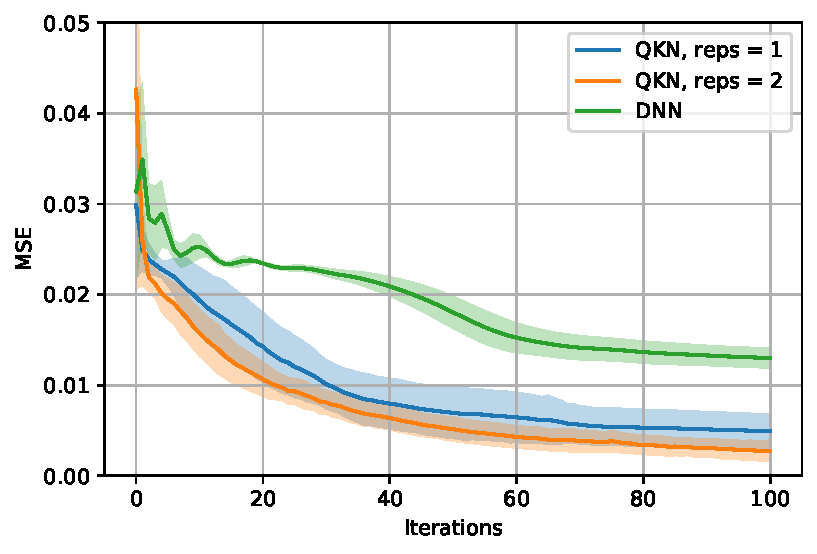
\includegraphics[height=1.9in]{latex/figures/3D_gaussian_data_fit.pdf}
        \caption{MSE of models trained on 3D mixed Gaussian data.}
        
    \end{subfigure}%
    \caption{MSE during training of the models defined in \autoref{tab:training models}, trained on the mixed Gaussian data (see \autoref{sec:Mixed Gaussian Data} for details on the data). The QNNs and QCNs are trained using ideal simulations, using the methods of \autoref{sec:Exact Expectation Value}.}
    \label{fig:trained ideal}
\end{figure}

\begin{table}[H]
\centering
\caption{Final MSE after training of the models detailed in \autoref{tab:training models}, using exact simulation. See \autoref{sec:Exact Expectation Value} for details. These results accompany the training shown in \autoref{fig:trained ideal}.}
\begin{tabular}{|l|l|l|l|l|}
\hline
Model& Type& Data& MSE, $10^{2}$ Epochs& MSE, $10^{4}$ Epochs \\ \hline
A    & QNN & 1D  &  $4.6\times 10^{-2}$  & NA   \\ \hline
B    & QCN & 1D  & $5.9\times 10^{-3}$  & NA \\ \hline
C    & QCN & 1D  & $\boldsymbol{8.0\times 10^{-4}}$  & NA  \\ \hline
D    & DNN & 1D  & $1.1\times 10^{-2}$ & $3.1\times 10^{-2}$  \\ \Xhline{2\arrayrulewidth}
E    & QNN & 2D  &  $3.6\times 10^{-2}$ & NA  \\ \hline
F    & QCN & 2D  &  $1.8\times 10^{-2}$ & NA  \\ \hline
G    & QCN & 2D  &  $\boldsymbol{4.3\times 10^{-3}}$ & NA  \\ \hline
H    & DNN & 2D  &  $2.5\times10^{-2}$ & $1.6\times10^{-3}$\\ 
\Xhline{2\arrayrulewidth}
I    & QNN & 3D  &  $2.0\times 10^{-2}$& NA  \\ \hline
J    & QCN & 3D  &  $4.9\times 10^{-3}$ & NA  \\ \hline
K    & QCN & 3D  &  $\boldsymbol{2.8\times10^{-3}}$  & NA  \\ \hline
L    & DNN & 3D  &  $1.2\times10^{-2}$  & $1.8\times10^{-3}$  \\ \hline
\end{tabular}
 
\label{tab:training models mse}
\end{table}

From \autoref{fig:trained ideal}, we see that the QCNs minimize the MSE quicker than both the QNNs and DNNs on the mixed Gaussian data, for any number of dimensions. The QCNs with the two ansatz repetitons also trained faster than those with just one. Further, we see that QNNs perform overall worst among the models. After initially fast optimization, the models quickly flatten out at a relatively high MSE, struggling to obtain a good fit. 

From \autoref{tab:training models}, we see that the DNNs obtains the lowest MSE among all models when trained until saturation, after $10^4$ epochs. The one exception to this was for the 1D mixed Gaussian data, where the MSE actually increased after the additional training for the DNN. This is likely due to heavy overparameterization for this model, having 13 nodes to achieve $20$ parameters, causing it to become very unstable.


%================================================================
\subsection{Noisy Simulation}\label{sec:Noisy Simulation}
%================================================================
In this subsection, we investigate how QNNs and QCNs behave when trained on the Gaussian data using simulated quantum hardware. We do this by repeating the training of the models of last subsection using a simulation of the Santiago quantum computer. We exclude, however, the training on the 3D mixed Gaussian due to the huge computational burden of simulating real hardware. The resulting MSE during training can be seen in \autoref{fig:trained noisy}. Each model was trained for 100 epochs, using 1024 shots to estimate the output of each circuit. \autoref{tab:training models mse noisy} shows the final MSE after 100 epochs for the QNNs and QCNs, trained on simulated hardware. As earlier, the resulting MSE after 100 and $10^{4}$ epochs is also included for the DNNs.


\begin{figure}[H]
    \centering
    \begin{subfigure}[t]{0.45\textwidth}
        \centering
        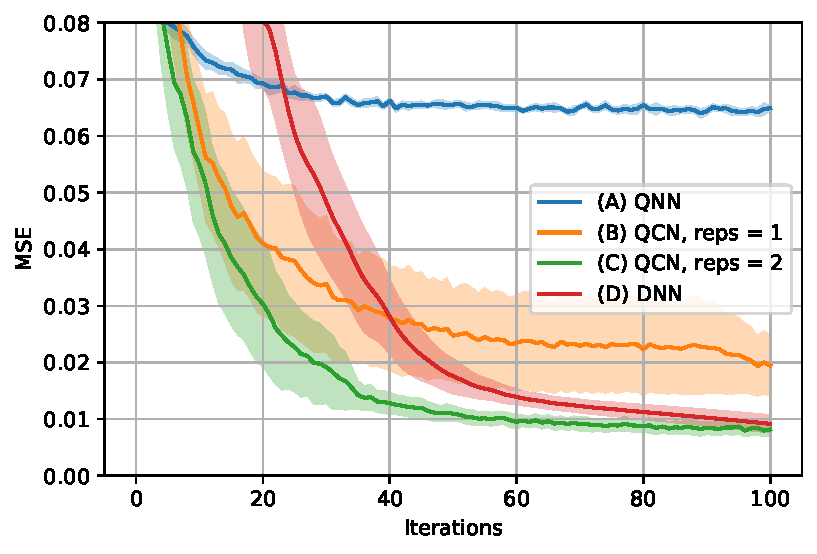
\includegraphics[height=1.9in]{latex/figures/1D_gaussian_data_fit_noisy.pdf}
        \caption{MSE of models trained on 1D mixed Gaussian data.}
        
    \end{subfigure}%
    \hfill 
    \begin{subfigure}[t]{0.45\textwidth}
        \centering
        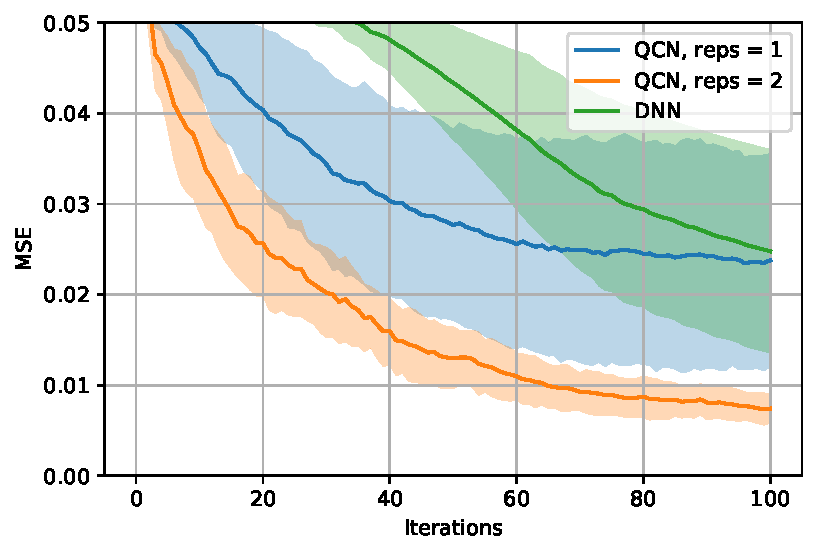
\includegraphics[height=1.9in]{latex/figures/2D_gaussian_data_fit_noisy.pdf}
        \caption{MSE of models trained on 2D mixed Gaussian data.}
    \end{subfigure}
    \caption{MSE during training of the models defined in \autoref{tab:training models}, trained on the mixed Gaussian data, excluding the 3D data (see \autoref{sec:Mixed Gaussian Data} for details on the data). The QNNs and QCNs are trained using noisy simulation of the Santiago quantum computer, using the methods of \autoref{sec:Noisy Simulation}.}
    \label{fig:trained noisy}
\end{figure}


\begin{table}[H]
\centering
\caption{Final MSE after training the models detailed in \autoref{tab:training models}, using noisy simulation of the Santiago quantum computer. See \autoref{sec:Noisy Simulation} for details. These results accompany the training shown in \autoref{fig:trained noisy}.} 
\begin{tabular}{|l|l|l|l|l|}
\hline
Model& Type& Data& MSE, $10^{2}$ Epochs& MSE, $10^{4}$ Epochs \\ \hline
A    & QNN & 1D  & $6.6 \times 10^{-2}$   & NA   \\ \hline
B    & QCN & 1D  & $2.0\times 10^{-2}$  & NA \\ \hline
C    & QCN & 1D  & $\boldsymbol{8.2\times 10^{-3}}$  & NA  \\ \hline
D    & DNN & 1D  & $1.1\times 10^{-2}$ & $3.1\times 10^{-2}$  \\ \Xhline{2\arrayrulewidth}
E    & QNN & 2D  &  $4.0 \times 10^{-2}$                  & NA  \\ \hline
F    & QCN & 2D  &  $2.4\times 10^{-2}$ & NA  \\ \hline
G    & QCN & 2D  &  $\boldsymbol{7.4\times 10^{-3}}$ & NA  \\ \hline
H    & DNN & 2D  &  $2.5\times10^{-2}$ & $1.6\times10^{-3}$\\\hline
\end{tabular}

\label{tab:training models mse noisy}
\end{table}

Comparing \autoref{fig:trained noisy} and \autoref{fig:trained ideal}, we see that the QNNs and QCNs trained on noisy hardware train slower and obtain a overall higher final MSE after 100 epochs, compared to the ideal simulation. 


%================================================================
\subsection{Discussion}\label{sec:Training Discussion}
%================================================================
In \autoref{sec:Vanishing Gradient Phenomenon} and \autoref{sec:Investigating the Loss Landscape}, it was suggested that QCNs of few qubits and layers would train faster than DNNs with similar number of parameters, due to their relatively larger gradient and more uniform EFIM spectrum. As we see from \autoref{fig:trained ideal}, this is indeed the case when training on the mixed Gaussian data using exact and noiseless simulation.
Further, we see that the QCNs with two ansatz repetitions show faster training and less variance than those with only one repetition. This shows that QCNs can be made more flexible by adding additional complexity to each node in the form of additional repetitions. 

In \autoref{sec:Expressivity}, it was suggested that QCNs are more expressive and flexible than DNNs with similar number of parameters. Looking at \autoref{tab:training models mse}, we see that the final MSE obtained by the QCNs with two repetitions is within the same order of magnitude as the final MSE obtained by the DNNs. This is despite the fact that the QCNs were only trained for 100 epochs, while the DNNs where allowed to train for $10^4$ epochs (basically until saturation, i.e. the lowest possible MSE for that particular model). In light of this, it is not unlikely that the QCNs would eventually reach a lower MSE than the DNNs if given the opportunity to train for more epochs. This suggests that it is possible for QCNs to fit complicated data more easily than DNNs, and hence are more flexible. However, this is speculative, as we are unable to train the QCNs much further due to limited computational resources.    

Even though QNNs with RZZ encoding were shown to also exhibit a relatively uniform EFIM spectrum in \autoref{sec:Investigating the Loss Landscape}, we see in \autoref{fig:trained ideal} that they struggle to obtain a good fit on the mixed Gaussian data, even though they have a similar number of parameters as the QCNs with one ansatz repetition. This shows that RZZ encoding combined with multiple repetitions of the simple ansatz is insufficient for fitting this data. As explained in \autoref{sec:FeedForward}, our QNNs perform a mostly unitary (and thus linear) transformation of the input, except at the stage of encoding and measurement. This results in a perhaps too constrained model, which might explain the QNNs' inability to fit the data. QCNs, on the other hand, incorporate multiple non-linearities for each layer as a result of measurements done to estimate the output of each node, as explained in \autoref{sec:Quantum Circuit Network}. As with DNNs, this is likely the key to their greater flexibility, as it enables them to compute a larger family of functions. 

Moving over to the training using the simulated noisy hardware, we see from \autoref{fig:trained noisy} that the QNN and QCN models performed overall worse than in the ideal case. This is not surprising, since the simulation of real hardware and the low number of 1024 shots cause a significant amount of noise to be added to the outputs of the QNNs and QCNs. The slowdown of the training is likely a due to noise being added to the calculation of the gradient. This causes it to misalign with the direction of steepest descent, as discussed in \autoref{sec:BarrenPlateus}, and which results in the optimization slowing down. However, the QCNs with two ansatz repetitions still obtained a lower MSE than the DNNs after 100 epochs, even in using the noisy simulation. This shows that QCNs have the ability to outperform DNNs on some data sets, even on noisy quantum hardware with few shots. 


%================================================================
\section{Real Data}\label{sec:Real Data}
%================================================================
In this this section, we compare the performance QCNs and DNNs by performing regression on the Boston Housing data (kilde) and classification on the Breast Cancer Wisconsin data (kilde). See \autoref{sec:Appendix B} for more information about the data sets. Since these data originate from real world experiments, they are noisy and don't represent a deterministic relationship $y = f(\boldsymbol{x})$ between the target and the features. This is in contrast to the the mixed Gaussian data sets studied earlier, and should provide a more practical benchmark of the methods. In addition to evaluating the models using MSE on the training data, we will also investigate how they generalize to unseen data by evaluating the MSE on an independent test set, as explained in \autoref{sec:Generalizability}. For the Breast Cancer Wisconsin data, we will also investigate the training and test accuracy \autoref{eq:accuracy} of the models.

In \autoref{sec:Feature Reduced Data}, we will reduce the number of features for data sets to four (down from $13$ and $30$, respectively) by using principal component analysis, as described in \autoref{sec:Principal Component Analysis}. This is done in order to produce smaller, more manage QCNs, as qubit encoding generally requires one qubit for each feature. The QCNs models are chosen to have four qubits in each circuit, and only two layers. This is done to obtain a model that has a large gradient due to low number of qubits, as discussed in \autoref{sec:Vanishing Gradient Phenomenon Discussion}, and are thus easy to train. The DNNs are chosen such that the number of parameters approximatly match that of the QCNs. 

In \autoref{sec:Hybrid Method}, we will repeat the experiments of \autoref{sec:Feature Reduced Data} on the data sets with all features present, i.e. without feature reduction. To avoid QCNs with overly many qubits, we will use an initial dense layer to reduce the features from $13$ and $30$ to four. This creates a DNN/QCN hybrid model, where the initial dense layer learns derived features on which the QCN part makes predictions. See \autoref{sec:Hybrid Models} for details. 

For both the feature reduced and full data set, we will split the data sets into independent training and test sets at random, each with $N=100$ samples. The targets of the Boston Housing data is min-max scaled to $y \in [0,1]$, while the discrete targets of the Breast Cancer data are already $y \in \{0,1\}$.

%================================================================
\subsection{Feature Reduced Data}\label{sec:Feature Reduced Data}
%================================================================
To reduce the number of features, the training and test data sets are each reduced to four features using PCA and scaled appropriately depending on the model, as explained in \autoref{sec:Pre-processing Input}. The hyperparameters of the various models trained on the feature reduced data is listed in \autoref{tab:training models PCA}.

\begin{table}[H]
\centering
\caption{Hyperparameters of the various models fitted to the feature reduced Boston Housing data and Breast Cancer data.} 
\begin{tabular}{|l|l|l|l|l|l|l|l|}
\hline
Model& Type& Data& Qubits& Reps& Layers & Nodes &$n_{\theta}$ \\ \hline
A    & QCN & Boston Housing Data  & 4     & 2  &2     & 4& 40   \\ \hline
B    & DNN & Boston Housing Data  & NA    & NA &2     & 6& 37 \\ \Xhline{2\arrayrulewidth}
C    & QCN & Breast Cancer        & 4     & 2  &2     & 4& 40  \\ \hline
D    & DNN & Breast Cancer        & NA    & NA &2     & 6& 37  \\ \hline
\end{tabular}

\label{tab:training models PCA}
\end{table}

%\autoref{fig:train PCA} shows the training and test MSE of the models defined in \autoref{tab:training models PCA} as they are fitted to the feature reduced Boston Housing data and Breast Cancer data. Each model is initialized ten times with different parameters, and trained individually for 100 epochs. The resulting MSE is averaged.

%\begin{figure}[H]
%    \centering
%    \begin{subfigure}[t]{0.5\textwidth}
%        \centering
 %       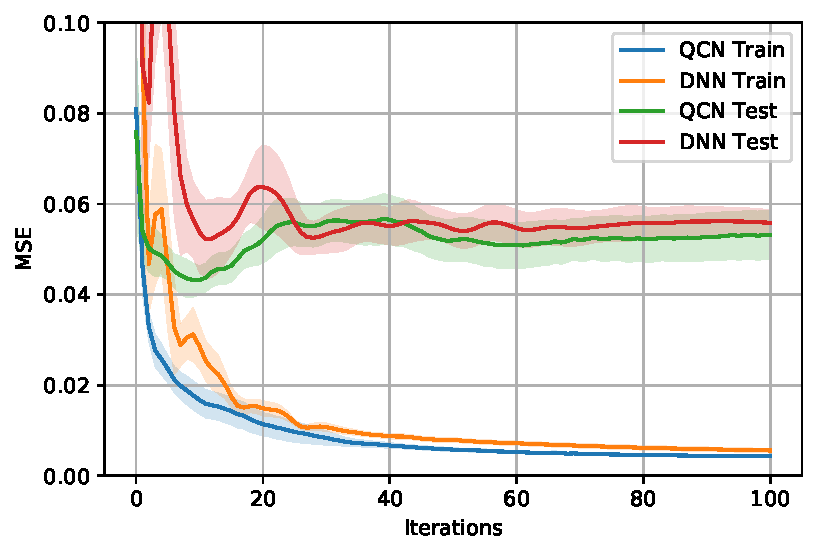
\includegraphics[height=1.9in]{latex/figures/Boston_PCA.%pdf}
%        \caption{Lorem ipsum}
%        
%    \end{subfigure}%
%    \hfill 
%    \begin{subfigure}[t]{0.5\textwidth}
%        \centering
%        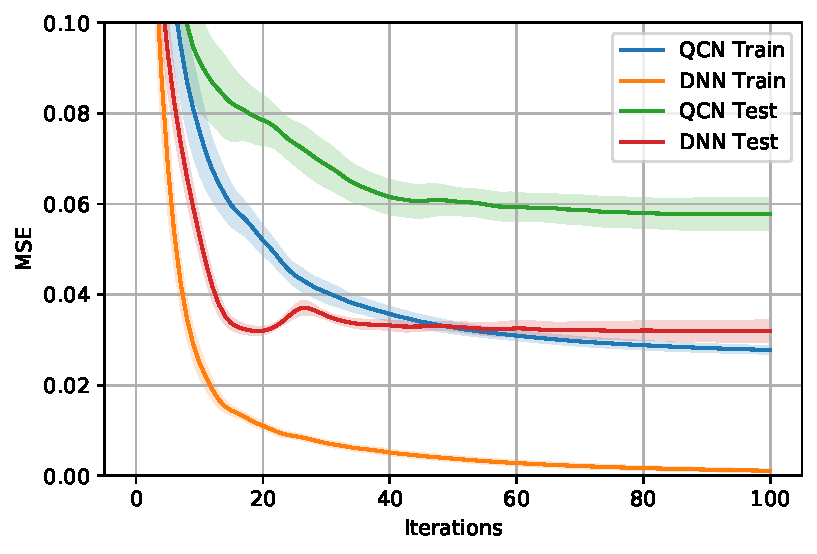
\includegraphics[height=1.9in]{latex/figures/Cancer_PCA.%pdf}
%        \caption{Lorem ipsum}
%    \end{subfigure}
%    \caption{Caption place holder}
%    \label{fig:train PCA}
%\end{figure}

The models defined in \autoref{tab:training models PCA} are trained for 100 epochs, ten times each for different random initializations of parameters.  In \autoref{tab:results PCA}, we see the average minimum training and test MSE for each model obtained during training. In addition, the final average training and test accuracy is included for the models trained on the Breast Cancer data. We see that the training MSE is strictly lower than the test MSE, i.e., both the QCN and DNN does not perform as good on the test set as on the training set. As explained in \autoref{sec:Generalizability}, we know that since the models are optimized with respect to the training set, its performance on the independent test set will always be worse. Comparing the models trained on the Boston Housing data, we see that the QCN has a lower test MSE than the DNN, meaning it generalizes better to unseen data. The same is however not true for the Breast Cancer data, where the QCN obtained almost twice the test MSE compared to the DNN. This indicates that the QCN is struggling to produce the correct labels $y^{(i)} \in \{0, 1\}$ which are the targets of the Breast Cancer data. Hence, both the train and test accuracies are lower for the QCN compared to the DNN. 
\begin{table}[H]
\centering
\caption{Hyper-parameters of the different models fitted to the Boston Housing data and Breast Cancer data.} 
\begin{tabular}{|l|l|l|l|l|}
\hline
Model& Type& Data& MSE (train/test)& Accuracy (train/test) \\ \hline
A    & QCN & BHD  & 0.004/$\boldsymbol{0.043}$ & NA    \\ \hline
B    & DNN & BHD  & 0.006/0.052                & NA  \\ 
\Xhline{2\arrayrulewidth}
C    & QCN & Breast Cancer        & 0.028/0.058                & 0.989/0.947    \\ \hline
D    & DNN & Breast Cancer        & 0.001/\boldsymbol{$0.032$} & 1.000/\boldsymbol{$0.965$}  \\ \hline
\end{tabular}

\label{tab:results PCA}
\end{table}


%================================================================
\subsection{Hybrid Method}\label{sec:Hybrid Method}
%================================================================
Using PCA for feature reduction enabled us to train feasibly small QCNs on the data, but in turn, we lost some of the information of the features. To enable us retain all the information of the data and train on all the features, we implement a hybrid model with an initial dense of the type \autoref{eq:FeedforwardSingle}. This layer  


\begin{table}[H]
\centering
\begin{tabular}{|l|l|l|l|l|l|l|l|}
\hline
Model& Type& Data& Qubits& Reps& Layers & Nodes &$n_{\theta}$ \\ \hline
E    & Hybrid & Boston Housing Data  & 4     & 2&3      & 4& 96   \\ \hline
F    & DNN & Boston Housing Data  & NA    & NA&3      & 5& 106 \\ \Xhline{2\arrayrulewidth}
G    & Hybrid & Breast Cancer        & 4     & 2&3      & 4& 164  \\ \hline
H    & DNN & Breast Cancer        & NA    & NA&3      & 5& 191  \\ \hline
\end{tabular}
\caption{Hyper-parameters of the different models fitted to the Boston Housing data and Breast Cancer data.} 
\label{tab:training models Hybrid}
\end{table}

%\begin{figure}[H]
%    \centering
%    \begin{subfigure}[t]{0.5\textwidth}
%        \centering
%        \includegraphics[height=1.9in]{latex/figures/Boston_Hyb%rid.pdf}
%        \caption{Lorem ipsum}
%        
%    \end{subfigure}%
%    \hfill 
%    \begin{subfigure}[t]{0.5\textwidth}
%        \centering
%        \includegraphics[height=1.9in]{latex/figures/Cancer_Hyb%rid.pdf}
%        \caption{Lorem ipsum}
%    \end{subfigure}
%    \caption{Caption place holder}
%    \label{fig:}
%\end{figure}

\begin{table}[H]
\centering
\begin{tabular}{|l|l|l|l|l|}
\hline
Model& Type& Data& MSE (train/test) & Accuracy (train/test) \\ \hline
E    & Hybrid & BHD  & 0.004/0.021 & NA    \\ \hline
F    & DNN & BHD     & 0.002/$\boldsymbol{0.011}$  & NA  \\ \Xhline{2\arrayrulewidth}
G    & Hybrid & BCD        & 0.035/0.102  & 1.000/0.875    \\ \hline
H    & DNN & BCD           & 0.000/$\boldsymbol{0.030}$  & 1.000/$\boldsymbol{0.954}$  \\ \hline
\end{tabular}
\caption{Hyper-parameters of the different models fitted to the Boston Housing data and Breast Cancer data.} 
\label{tab:results PCA}
\end{table}

%================================================================
%\section{Regularized Feature Map}\label{sec:Regularized Feature Map}
%================================================================
%Stuff

%================================================================
%\subsection{Discussion}\label{sec:Regularized Feature Map Discussion}
%================================================================
%Stuff


%==========================================================
%------------ part 4: conclusion & future -----------------
%==========================================================

\part{Conclusion \& Future Research}
%-------------------- placeholder --------------------
%================================================================
\chapter{Conclusion \& Future Research}\label{chap:Conclusion}
%================================================================

%----------------------------------------------------------------
\section{Conclusion}\label{sec:conclusion}
%----------------------------------------------------------------


%----------------------------------------------------------------
\section{Future Research}\label{sec:future}
%----------------------------------------------------------------


%----------------------------------------------------------------
\section{Todo}\label{sec:todo}
%----------------------------------------------------------------

\begin{itemize}
    \item Noise simulation only an approximation
\end{itemize}

%==========================================================
%--------------------- appendices -------------------------
%==========================================================

\appendix           % "Chapter" is renamed "Appendix"
\part*{Appendices}
\addcontentsline{toc}{part}{Appendices}


%\appendixpage       % Similar to \part*{Appendices}, but appears in TOC

%--------------------- appendix A --------------------
%================================================================
\chapter{DNN/QCN Hybrid}\label{sec:Appendix A}
%================================================================

%================================================================
\subsection{Hybrid Method}\label{sec:Hybrid Method}
%================================================================
In \autoref{sec:Hybrid Method}, we will repeat the experiments of \autoref{sec:Feature Reduced Data} on the data sets with all features present, i.e. without feature reduction. To avoid QCNs with overly many qubits, we will use an initial dense layer to reduce the features from $13$ and $30$ to four. This creates a DNN/QCN hybrid model, where the initial dense layer learns derived features on which the QCN part makes predictions. See \autoref{sec:Hybrid Models} for details.

Using PCA for feature reduction enabled us to train feasibly small QCNs on the data, but in turn, we lost some of the information of the features. To enable us retain all the information of the data and train on all the features, we implement a DNN/QCN hybrid model with an initial dense of the type \autoref{eq:FeedforwardSingle}. This layer  


\begin{table}[H]
\centering
\begin{tabular}{|l|l|l|l|l|l|l|l|}
\hline
Model& Type& Data& Qubits& Reps& Layers & Nodes &$n_{\theta}$ \\ \hline
E    & Hybrid & Boston Housing Data  & 4     & 2&3      & 4& 96   \\ \hline
F    & DNN & Boston Housing Data  & NA    & NA&3      & 5& 106 \\ \Xhline{2\arrayrulewidth}
G    & Hybrid & Breast Cancer        & 4     & 2&3      & 4& 164  \\ \hline
H    & DNN & Breast Cancer        & NA    & NA&3      & 5& 191  \\ \hline
\end{tabular}
\caption{Hyper-parameters of the different models fitted to the Boston Housing data and Breast Cancer data.} 
\label{tab:training models Hybrid}
\end{table}

%\begin{figure}[H]
%    \centering
%    \begin{subfigure}[t]{0.5\textwidth}
%        \centering
%        \includegraphics[height=1.9in]{latex/figures/Boston_Hyb%rid.pdf}
%        \caption{Lorem ipsum}
%        
%    \end{subfigure}%
%    \hfill 
%    \begin{subfigure}[t]{0.5\textwidth}
%        \centering
%        \includegraphics[height=1.9in]{latex/figures/Cancer_Hyb%rid.pdf}
%        \caption{Lorem ipsum}
%    \end{subfigure}
%    \caption{Caption place holder}
%    \label{fig:}
%\end{figure}

\begin{table}[H]
\centering
\begin{tabular}{|l|l|l|l|l|}
\hline
Model& Type& Data& MSE (train/test) & Accuracy (train/test) \\ \hline
E    & Hybrid & BHD  & 0.004/0.021 & NA    \\ \hline
F    & DNN & BHD     & 0.002/$\boldsymbol{0.011}$  & NA  \\ \Xhline{2\arrayrulewidth}
G    & Hybrid & BCD        & 0.035/0.102  & 1.000/0.875    \\ \hline
H    & DNN & BCD           & 0.000/$\boldsymbol{0.030}$  & 1.000/$\boldsymbol{0.954}$  \\ \hline
\end{tabular}
\caption{Hyper-parameters of the different models fitted to the Boston Housing data and Breast Cancer data.} 
\label{tab:results PCA}
\end{table}

%================================================================
%\section{Regularized Feature Map}\label{sec:Regularized Feature Map}
%================================================================
%Stuff

%================================================================
%\subsection{Discussion}\label{sec:Regularized Feature Map Discussion}
%================================================================
%Stuff


%--------------------- appendix B --------------------
%================================================================
\chapter{Abbreviations and Units}\label{sec:Appendix B}
%================================================================

%----------------------------------------------------------------
\section{List of Abbreviations}
%---------------------------------------------------------------

\begin{abbreviations}
    \item[AURKA] Aurora Kinase A
    \item[AURKB] Aurora Kinase B
    \item[AURKC] Aurora Kinase C
    \item[CDK] Cyclin-Dependent Kinase
    \item[CHARMM] Chemistry at HARvard Macromolecular Mechanics
    \item[CML] Chronic Myelogenous Leukemia 
    \item[CPC] Chromosomal Passenger Complex
    \item[DOF] Degrees of Freedom
    \item[EGFR] Epidermal Growth Factor Receptor
    \item[GROMACS] GROningen MAchine for Chemical Simulations
    \item[HDX] Hydrogen-Deuterium Exchange
    \item[INCENP] Inner Centromere Protein
    \item[MD] Molecular Dynamics
    \item[MS] Mass Spectrometry
    \item[NMR] Nuclear Magnetic Resonance
    \item[PBC] Periodic Boundary Conditions
    \item[PCA] Principal Component Analysis
    \item[PK] Protein Kinase
    \item[PKA] Protein Kinase A
    \item[RMSD] Root-Mean-Square Deviation
    \item[RMSF] Root-Mean-Square Fluctuation
    \item[VMD] Visual Molecular Dynamics
\end{abbreviations}

%----------------------------------------------------------------
\section{Units}
%---------------------------------------------------------------
\begin{table}[H]
\caption*{}
\centering
%\rowcolors{2}{gray!15}{white}
\addtolength{\tabcolsep}{7pt} 
\begin{tabular}{ll}
\hline
M & molar (1 mol/L)
\\
$\mu$s & microsecond ($10^{-6}$ s)
\\
ns & nanosecond ($10^{-9}$ s)
\\
ps & picosecond ($10^{-12}$ s)
\\
Å & Ångström ($10^{-10}$ m)
\\
\hline
\end{tabular}
\addtolength{\tabcolsep}{7pt} 
\label{tab:units}
\end{table} 


%==========================================================
%-------------------- bibliography-------------------------
%==========================================================
\newpage 
\printbibliography[heading=bibintoc, title={References}]


\end{document}
%==========================================================
% ------------------- END OF MAIN CONTENT -----------------
%==========================================================
